% http://www.idsc.ethz.ch/education/theses-semester-projects.html
% IDSC LaTeX Thesis Template
% 
% Author(s):	Eric Müller
% 				Institute for Dynamic Systems and Control
% 				Swiss Federal Institute of Technology (ETH) Zurich
% 
% Created:		2004/04/02  (Eric Mueller)
% 
% Notes: Has been tested on Windows 7 + MikTeX + TeXnicCenter
%
% Revisions: 	2009/05/29  (Soren Ebbesen)
% 				    2011/03/22	(Soren Ebbesen)
%             2013/03/08	(Soren Ebbesen)
%             2014/03/13	(Soren Ebbesen)
% ______________________________________________________________________________
\documentclass[12pt,oneside,a4paper,fleqn]{report}
% \setcounter{secnumdepth}{3}

\usepackage[cmex10]{amsmath}

\usepackage{titlesec}
\titleformat{\chapter}
  {\normalfont\Huge\bfseries}{\thechapter}{1em}{}
\titlespacing*{\chapter}{0pt}{3.5ex plus 1ex minus .2ex}{2.3ex plus .2ex}

\usepackage{float}
\usepackage{graphicx}
\graphicspath{ {img/} }

\usepackage[table,xcdraw]{xcolor}

\usepackage{enumitem}

\usepackage{epigraph}

\usepackage{tocbibind}

\usepackage{csquotes}
\usepackage{relsize,etoolbox}
\AtBeginEnvironment{quote}{\smaller}

\usepackage[font=footnotesize,labelfont=bf]{caption}


\usepackage[english,mt]{ethidsc} % Special IDSC styles and commands      	
								 % {german}/english: language of headings, etc.
								 % {st}/bt/mt: {semester}/bachelor/master thesis


\usepackage{float}
\restylefloat{table}

\usepackage{listings}
\lstset{
  basicstyle=\fontsize{10}{12}\selectfont\ttfamily,
  columns=fullflexible,
  breaklines=true,
  postbreak=\mbox{{$\hookrightarrow$}\space},
}
% *** PDF, URL AND HYPERLINK PACKAGES ***
%
\usepackage{url}
\usepackage{cleveref}
\usepackage{indentfirst}

\usepackage{bussproofs}

\fancyhf{}
						
% Page header (don't change)____________________________________________________
\setlength{\parindent}{0em}                 % Disable parindent
\rhead[\small\nouppercase{\rightmark}]{\thepage}  % Special headings
\lhead[\small\thepage]{\nouppercase{\leftmark}}   % Special headings
\cfoot{}                                    % Special headings


% Title page (please fill in)___________________________________________________
\title{Functional Programming Applied to \\ Electromagnetic Transient Analysis \\ (short-document version)}


\studentA{Hanneli Carolina Andreazzi Tavante}
\ethidA{}
\semesterA{4}
\emailA{hannelita@gmail.com}

%\studentB{Second Student}
%\ethidB{12-345-678}
%\semesterB{9}
%\emailB{second@student.ethz.ch}

\committees{Prof. Dr. Fernando Nunes Belchior \\ Federal University of Goias, Brazil \\ Prof. Dr. Edmilson Marmo Moreira \\ Federal University of Itajuba, Brazil}

\supervision{Main Supervisor\\ Prof. Ph.D. Benedito Donizetti Bonatto \\Co-Supervisor\\ Prof. Ph.D. Maurilio P. Coutinho}
\date{December 2019}

\identification{2018100494} 		% Project identifier

% \infopage
% \declaration

% Begin document________________________________________________________________
\begin{document}

\maketitle 							% Create title page


% Preamble______________________________________________________________________

\pagenumbering{roman} 				% Begin roman page numbering (i,ii,...)

%---------------------------------------------------------------------------
% Preface


\chapter*{Acknowledgements}
  \addcontentsline{toc}{chapter}{Acknowledgements}

A chain of unexpected events and some unexpected people around the world brought me here. I wouldn't be writing this page if my supervisors, Dr. B. Bonatto and Dr. M. Coutinho hadn't accepted me as their student. I kindly thank them for their endless patience with my hyperactive behaviour towards science. They were the best people to deal with the unusual ideas I proposed during these two years as a MSc student.
\\

I also thank our University, UNIFEI, for being there all the time, during my bachelor's and during my graduate studies. In times when truths and tautologies are threatened, resisting to ignorance is a brave act.
\\

Last but not least, I wouldn't have gone far if my two best friends, A. A. and A. A. (what a coincidence for these abbreviations!) hadn't been supporting me for the last decade or so. And most importantly, to my family, V. R and I. R. 
\\

H. C. A. Tavante




 \cleardoublepage

\chapter*{}

\renewcommand{\epigraphsize}{\footnotesize}
\epigraph{``It was not by making yourself heard but by staying sane that you carried on the human heritage.''}{George Orwell}

\cleardoublepage

%---------------------------------------------------------------------------
% Table of contents

 \setcounter{tocdepth}{2}
 \tableofcontents

 \cleardoublepage

%---------------------------------------------------------------------------
% Abstract
\chapter*{Abstract}
 \addcontentsline{toc}{chapter}{Abstract}

Many engineering projects rely on software to execute simulations and analysis of a wide variety of domains. Computer programs are great allies of the engineers when it comes to simulations, including the ones for electromagnetic transient analysis. However, a single programming paradigm (the imperative paradigm) seems to have dominated most of the commercial and academic applications. 
\\

This work presents and implements an algorithm to analyse simple electromagnetic transient circuits adopting functional programming. The code uses the nodal analysis found on industry programs like the EMTP (Electromagnetic Transients Program). The results of adopting the Haskell language and functional programming are very favourable to the engineering community: programs with higher chances to have fewer bugs, with concise implementations and with more focus on the mathematical aspects of the algorithm.
\\

\textbf{Keywords}: Functional programming, electromagnetic transient analysis, Haskell, programming languages.



 \cleardoublepage

%---------------------------------------------------------------------------
% Symbols

% \chapter*{Nomenclature}\label{chap:symbole}
%  \addcontentsline{toc}{chapter}{Nomenclature}

% \section*{Symbols}
% \begin{tabbing}
%  \hspace*{1.6cm} \= \hspace*{8cm} \= \kill
%  $\mathrm{EHC}$ \> Conditional equation \> [$-$] \\[0.5ex]
%  $e$ \> Willans coefficient \> [$-$] \\[0.5ex]
%  $F,G$ \> Parts of the system equation \> [\unitfrac[]{K}{s}]
% \end{tabbing}

% \section*{Indicies}
% \begin{tabbing}
%  \hspace*{1.6cm}  \= \kill
%  a \> Ambient \\[0.5ex]
%  air \> Air
% \end{tabbing}

\section*{Acronyms and Abbreviations}
\begin{tabbing}
 \hspace*{1.6cm}  \= \kill
 CDA \> Critical Damping Adjustment \\[0.5ex]
 CSV \> Comma-separated values  \\[0.5ex]
 ETR-P \> Electromagnetic Transient Program \\[0.5ex]
 GHC \> Glasgow Haskell Compiler   \\[0.5ex]
 GHCi \> Glasgow Haskell Compiler interactive  \\[0.5ex]
 GUI \> Graphical User Interface  \\[0.5ex]
 I/O \> Input/Output \\[0.5ex]
 JSON \> JavaScript Object Notation \\[0.5ex]
 PoC \> Proof of Concept \\[0.5ex]
 THTA \> Trapezoidal History Term Averaging \\[0.5ex]
 UNIFEI \> Universidade Federal de Itajuba \\[0.5ex]
 UBC \> University of British Columbia \\[0.5ex]
 UI \> User Interface \\[0.5ex]

\end{tabbing}

\listoftables

\listoffigures

\lstlistoflistings

\cleardoublepage

\parskip 0.5ex plus 0.2ex minus 0.1ex

\parindent    1.0em


%---------------------------------------------------------------------------


% Chapters______________________________________________________________________

\pagestyle{fancy}               	% Fancy headings
\pagenumbering{arabic}				% Begin arabic page numbering (1,2,...)

\chapter{Introduction}
\label{sec:introduction}

\section{Motivation}

Computer-aided applications play a crucial role in engineering. Since the 1950s, many engineering projects rely on software to execute simulations and analysis of a wide variety of domains. Engineering (Civil, Mechanical, Electrical) has a heavy focus on mathematical models, time optimisations and new applications for modern techniques. Nevertheless, in many situations, engineers of these domains do not spend much time investigating a vital tool at the development of computer software: programming languages. 

One of the earliest and most concise definitions of programming languages comes from \cite{sammet1972programming}. 
\begin{quote}
"[A Programming Language] is considered to be a set of characters and rules for combining them which have the following characteristics: (1) machine code knowledge is unnecessary; (2) there is good potential for conversion to other computers; (3) there is an instruction explosion (from one to many); and (4) there is a notation which is closer to the original problem than assembly language would be".
\end{quote}


The core of software engineering for industrial applications started with the Assembly language, moving towards more structured languages like Fortran, Algol, Cobol, PL/I, Basic, Pascal, C, Smalltalk, Prolog, C++, Matlab, and more recently, Python, R and Java \cite{parker2012history}. However, it is possible to find a much broader spectrum of programming languages as illustrated in Figure \ref{histprog} (source \cite{ibmpl}).

\begin{figure}[H]
   \centering
   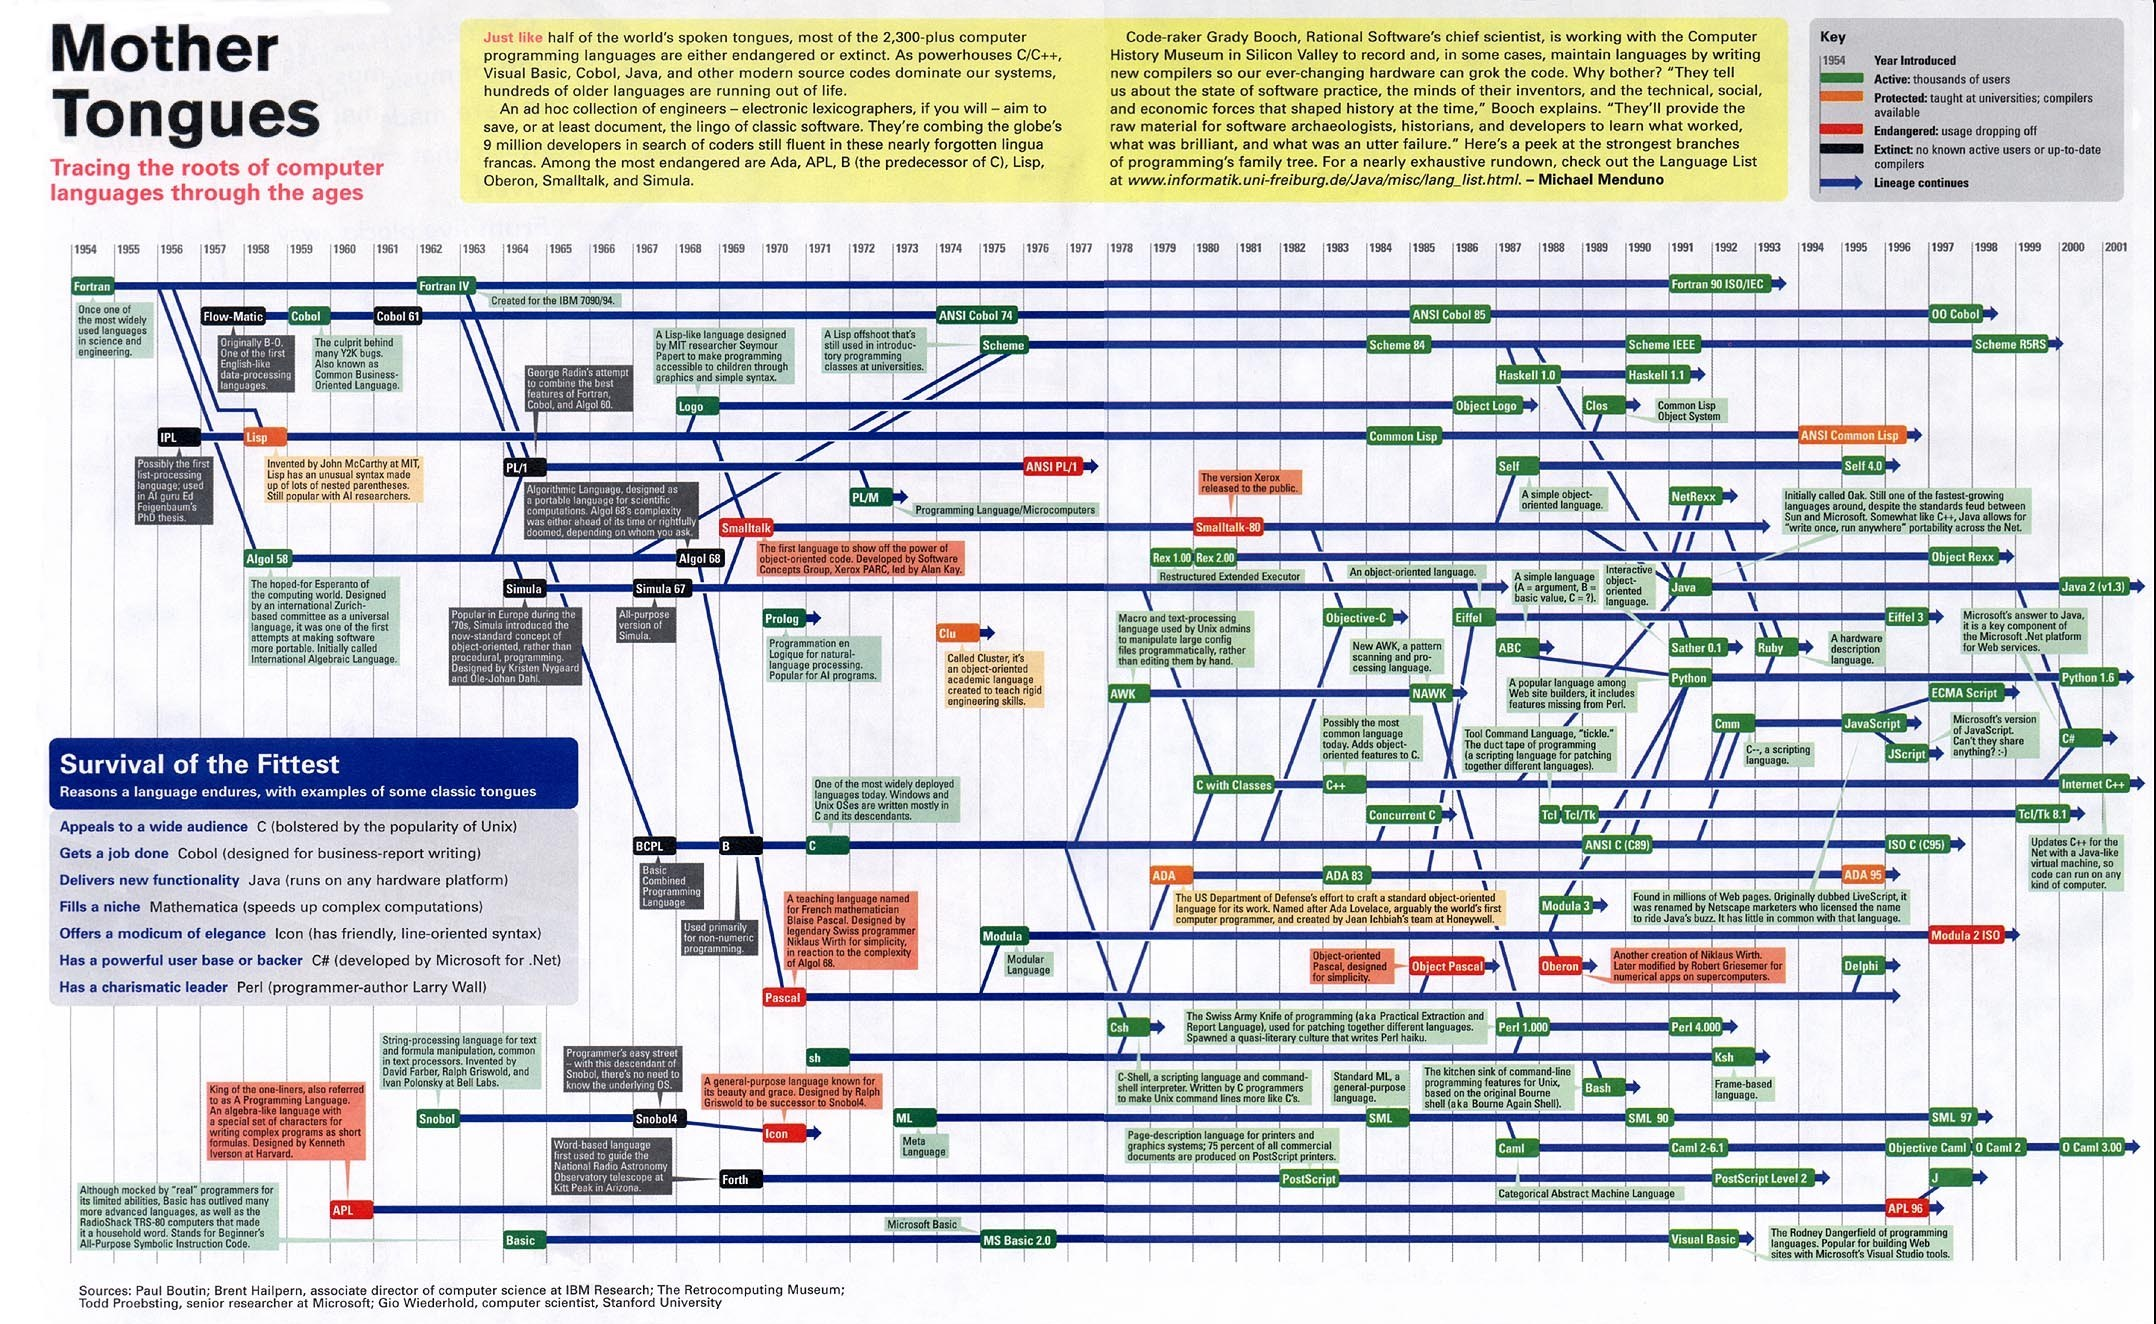
\includegraphics[angle=90,origin=c,width=0.95\textwidth]{img/histprog.jpeg}
   \caption{Programming languages history summary}
   \label{histprog}
\end{figure}


Programming languages itself is a dense topic, branching into compilers, static analysis, program synthesis, proofs, concurrency, type theory, logic and many others. Programming languages also have different paradigms \cite{felleisen2018design}. Historically speaking, the industry has been adopting procedural and \textbf{imperative} styles during the majority of the time.

\textbf{Imperative programming} is a paradigm that describes computation as statements - they can modify the state of the program. These statements focus on how they should solve the problem proposed in the algorithm, requiring a detailed instruction guide to perform.

There are different programming paradigms apart from the imperative style. Some languages follow the \textbf{Functional programming} paradigm - "they are descriptive rather than imperative, have no assignment command and no explicit flow of control - subcomputations are ordered only partially, by data dependency"\cite{turner2006church}. The principal component in this alternative paradigm is the application of a function to its arguments, not the computation of statements.   


\section{Research goals}
\label{rgoals}

This work proposes the adoption of the functional programming paradigm with a functional programming language to build a simple program reproducing a well-known algorithm for electromagnetic transient analysis of simple electrical circuits. This baseline algorithm uses a didactic program, developed in the MatLab plataform, by students at UNIFEI and UBC (see \cite{thtaoctave}). It aims to answer the following questions:



\begin{enumerate}
  \item What are the benefits of using a functional programming language? Will the development process be more intuitive? Will it be possible to apply all the functional programming concepts directly into the application domain? 
  \item What will be the differences with respect to the code base? Will it be shorter or longer? Will it produce a readable code?
  \item What will be the technical challenges? Functional programming is becoming more popular in the industry only in recent years, so there are not many documents and articles available to report challenges during the development process of engineering applications.
  \item How and why "functional languages are associated with fewer defects than either procedural or scripting languages"\cite{ray2014large}?
\end{enumerate}

The development of the Haskell application will answers the questions previously proposed.

Some of the complementary goals of this project are listed below.

\begin{itemize}
  \item Create an open-source implementation of a project using a real-world engineering application (electromagnetic transients) applying functional programming. There are not many projects in electrical engineering using this paradigm and this work can be a basic reference project for future research on similar topics.
  \item A software developer of electrical engineering applications should care about the tools he/she adopts. The programming language chosen is one of the main tools of the project. The selection of an inappropriate tool leads to bugs and unwanted behaviour. The correctness of the program also relies on the programming language. A professional software engineer will consider this matter when delivering a project.
\end{itemize}

\section{Relevance}

The future of engineering applications is strictly connected to advances in computer science and software development. Still, these two areas are mostly treated as entirely separate domains. This work aims to build a bridge between programming languages (with a case study on functional programming) and electrical engineering (with electromagnetic transient analysis).

The domain of programming languages research is vast. Analysing the use of functional programming for electrical engineering applications is just a starting point. This work is relevant because it can open doors for several future outputs, such as type analysis focused on the most common engineering models, formal verification of algorithms (increasing the reliability of the delivered software), and so on. Expanding this analysis to a field called Type Theory may lead to exciting results - would it be possible to guarantee that the written algorithm is mathematically equivalent to the engineering model? There are not many publications in this domain yet. Functional programming is the entry point for a more in-depth analysis of this matter.

\section{Methodology}

After a literature review on functional programming, Haskell (the functional language chosen to be the primary tool of this work) and existing applications, a working software containing the proof of concept (PoC) will be delivered and it will be publicly accessible on Github (a Git repository hosting service with free plans).

Once the PoC is done, its results will be compared with the ones produced by Matlab version, validating if the algorithm produces values at least similar to the ones produced by the Matlab version. A comparison between code paradigms will follow the numerical results.

Octave (an open-source implementation of Matlab) is used to run the simulations from the imperative implementation; Stack\cite{stack} and Cabal\cite{cabal} are used with GHC to compile and run the Haskell version. 

\section{Chapters Overview}

Chapter \ref{ch:etr} gives an overview of the Nodal Analysis in Electromagnetic Transient Analysis, as well as a historical context of the software build for this domain, both in industry and in academia.

Chapter \ref{fp} presents the most important concepts of functional programming. It will provide the reader with conceptual examples and possible applications. It uses the actual code from the Haskell program developed in this work.

Chapter \ref{haskell} applies the functional programming concepts described in the previous chapter to the Haskell language, providing a rich set of practical applications in the language. Haskell is not the only functional language available; there are others like OCaml, SML, Racket. Two separates chapters were kept in order to emphasise that learning functional programming is different from learning Haskell (although it is a necessary to know both for delivering good quality software and the results of this work).

Chapter \ref{implhs} provides a thorough explanation of the Haskell application. In every section of this chapter, there is a recap of the main algorithm for electromagnetic transient analysis, a walk-through the Haskell code and comparisons with the original didactic program developed in MatLab.

Chapter \ref{results} presents the results of the implementation, numerically comparing the values obtained from complete simulations in both versions, Haskell and Matlab. It then compares the development process for both of the paradigms, functional and imperative.

Chapter \ref{conclusions} answers the questions proposed at \ref{rgoals}. It also provides an extensive list of future work and a contribution guide for researches interested in the topic.
 
% Future work is also reported on the appendices. They provide the reader with an introduction to Lambda-calculus (\ref{sec:lc}), logic (\ref{sec:logic}) and type analysis (\ref{sec:proofs}).







\cleardoublepage
% \chapter{Context: Software in Electrical Engineering }

[first software - allow ee projects; written with the languages we had; fortran
Appendix - all the prog. languages; history]

\section{ Languages }

The choice of which programming languages should be taught in computer science and engineering undergraduate programs varies from place to place. According to \cite{mason2018language}, Java and Python are popular choices in the UK and in Australia. Several articles suggest which should be the base language to be adopted considering students with no previous background in programming. \cite{wang2006practical} suggests PHP and Javascript, leaning toward a practical approach by developing web applications. The IEE Spectrum listed their most popular languages in 2015 (\cite{cass20152015}). In many cases, the object oriented programming model \cite{rumbaugh1991object} is the choice for the lectures. The main concepts are translated into classes and associations, with attributes and methods, generally using the imperative style (statements change the program's state). A deep analysis of the object oriented model is not in the scope of this work, but it is important to notice its wide adoption as a first contact with programming in general - and yet, this teaching formula might have complications (see \cite{kolling1999problem}; this article points out some issues with Objected Oriented programming and the imperative style, such as safety - mutable states may be a bad option in some scenarios - , syntax - some languages, such as C++, may have complex syntax for beginners - , etc).


Many courses neglect the existence of other styles and models, indirectly biasing the students to the same solution - object oriented programming and imperative code.

\section{ Alternative styles and languages }

\section{ How to choose a programming language }

[TODO - intro paragraph]

Type systems are tools for reasoning about programs \cite{pierce2002types}. Each programming language has its own type system, and it guarantees that a well-typed program is free of a certain group of misbehaviours. Type systems help with error detection, abstraction, documentation, language safety (protect its own abstractions of unexpected behaviours) and efficiency.



\cleardoublepage

\chapter{ Electromagnetic Transients }
\label{ch:etr}

The simulation and analysis of electromagnetic transients in basic electric circuits are essential to the study of power systems. Electromagnetic transient analysis software can help to determine overcurrent, overvoltage and other unwanted phenomena in power systems.  Since the 1970s, computer-aided algorithms have been developed to simulate a wide variety of conditions on complex circuits. 


\blockquote[\cite{martinez2015introduction}]{
Despite the powerful numerical techniques, simulation tools and graphical user interfaces currently
available, those involved in electromagnetic transients studies, sooner or later, face the limitations of
models available in transients packages, the lack of reliable data and conversion procedures for parameter
estimation or insufficient studies for validating models
}

Some of these simulation tools are well-known in industry and academia, such as ATP and EMTP. These two programs operate by creating a representation of the equivalent input circuit and obtaining the simulation results either by state space or nodal analysis. This work is focused on the latter approach.

\section{ Overview of Nodal Analysis }
\label{solutionalg}

Broadly studied at electromagnetic transients courses and firstly described by H. Dommel in \cite{dommel1969digital}, the nodal admittance matrix method is the base algorithm for programs like EMTP and ATP. This representation can deal with both single and multi-phase circuits containing resistors, capacitors, sources and a few other nonlinear elements as well as the discretization of the circuit differential equations through the trapezoidal integration method.


Figure \ref{transient1} illustrates a simple circuit and the continuous time domain first order differential equation and its solution for the current as function of time, considering the time constant (L/R) of the circuit.


\begin{figure}[H]
  \caption{Transient Analysis - Example Circuit}
  \centering
  \begin{minipage}[c]{0.59\linewidth}  
  %\subfloat{
    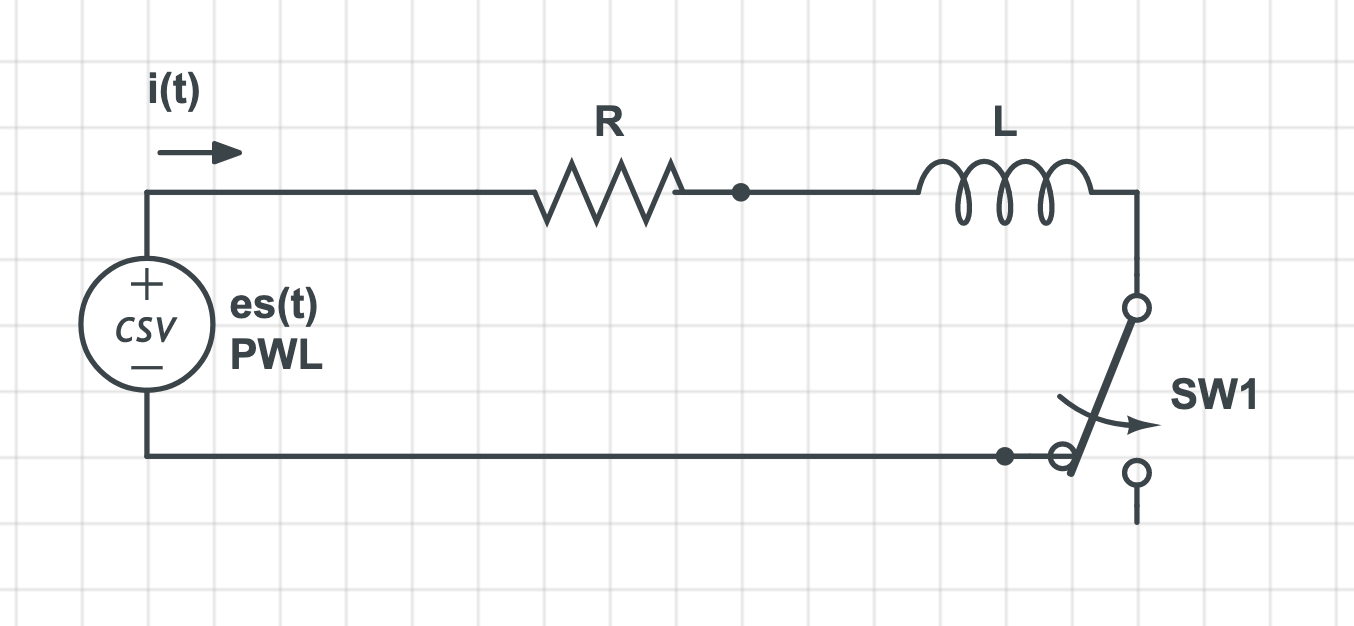
\includegraphics[width=1\linewidth]{img/transient1.png}
  %}
  \end{minipage}
  \hfill
  \begin{minipage}[c]{0.3\linewidth}
  % \subfloat{
    %}
  \end{minipage}  
  \label{transient1}
\end{figure}


\begin{subequations}
  \begin{equation}
    Ri + L \frac{di}{dt} = es(t)
  \end{equation}
  \begin{equation}
    i(t) = \frac{E}{R}[1 - e^{\frac{-t}{T}}]
  \end{equation}
  \begin{equation}
    T = \frac{L}{R}
  \end{equation}
\end{subequations}


When transforming the equation previously described in an algorithm, it is necessary to adopt discrete intervals of time $ \Delta t $, since digital computers are not able to simulate the idea of continuous-time. 

Assuming the single-phase case, \cite{dommel1969digital} describes the discrete representations for the inductors and the capacitor components, based on the trapezoidal numerical method integration:


\begin{figure}[H]
  \caption{Inductor - equivalent discrete representation}
  \centering
  \begin{minipage}[c]{0.59\linewidth}  
  %\subfloat{
    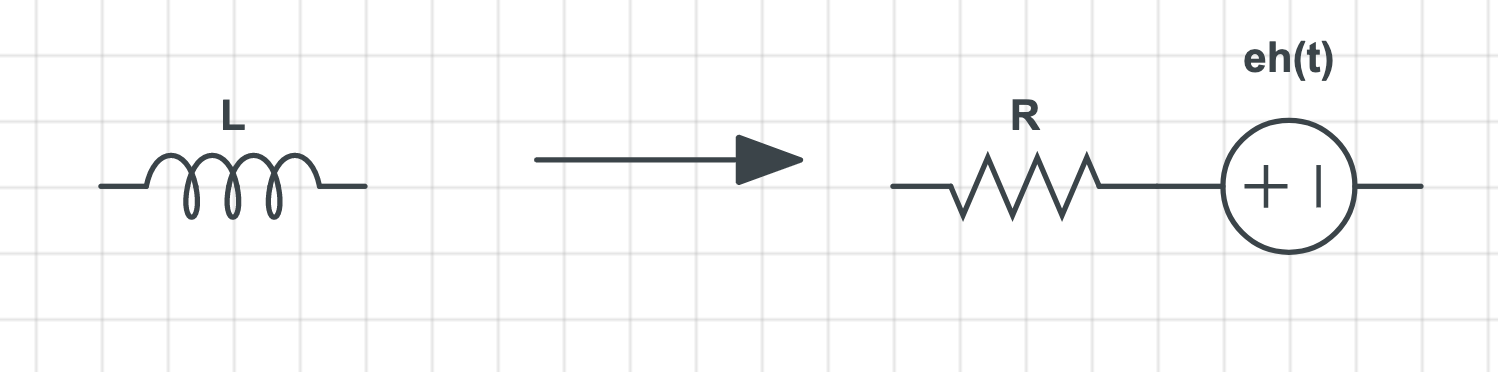
\includegraphics[width=1\linewidth]{img/Lequiv.png}
  %}
  \end{minipage}
  \hfill
  \begin{minipage}[c]{0.3\linewidth}
  % \subfloat{
    
    %}
  \end{minipage}  
  \label{transient2}
\end{figure}

\begin{subequations}
  \begin{equation}
    R = \frac{2 L}{\Delta t}
  \end{equation}
  \begin{equation}
    eh(t) = -V (t - \Delta t) - \frac{2 L}{\Delta t} i (t - \Delta t)
  \end{equation}
\end{subequations}


\begin{figure}[H]
  \caption{Capacitor - equivalent discrete representation}
  \centering
  \begin{minipage}[c]{0.59\linewidth}  
  %\subfloat{
    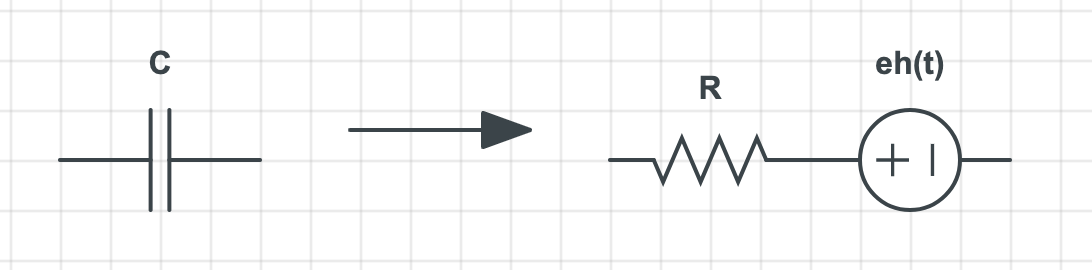
\includegraphics[width=1\linewidth]{img/Cequiv.png}
  %}
  \end{minipage}
  \hfill
  \begin{minipage}[c]{0.3\linewidth}
  % \subfloat{
    %}
  \end{minipage}  
  \label{transient3}
\end{figure}

\begin{subequations}
  \begin{equation}
    R = \frac{\Delta t}{2 C}
  \end{equation}
  \begin{equation}
    eh(t) = V (t - \Delta t) + \frac{\Delta t}{2 C} i (t - \Delta t)
  \end{equation}
\end{subequations}


Other numerical methods can be taken into consideration. Each distinct numerical method can generate different equivalent values for the limped L and C components. The trapezoidal integration method has been used in academic and commercial EMTP-based programs mainly due to its accuracy and stability properties. Analysing the advantages or disadvantages of each method is out of the scope of this work.

\section { EMTP algorithm }

Into EMTP or ATP software, the discrete models previously described compose a matrix equation in the following format:

\begin{figure}[htb]
  \caption{Nodal matrix model}
  \centering
  
  % \subfloat{
    \begin{subequations}
      \begin{equation}
        [G][V] = [h]
      \end{equation}
      % \begin{equation}
      %   eh(t) = V (t - \Delta t) + \frac{\Delta t}{2 C} i (t - \Delta t)
      % \end{equation}
    \end{subequations}
    %}
  \label{transient3}
\end{figure}

At \ref{transient3}, $ G $ is the matrix of conductances, $ V $ is the vector of unknown voltages and $ h $ is the vector of known current sources (independent current sources and the historical equivalent current sources).

It is possible to state a general algorithm \cite{dommel1969digital} in electromagnetic transients analysis according to the following procedures:
\begin{enumerate}
  \item Read the input data;
  \item Build the steady-state solution matrix;
  \item Build the transient solution matrix (G);
  \item Find the steady-state solution to initialise histories;
  \item Assume $ t = \Delta t $;
  \item \label{evaluateh} Evaluate current and voltage sources; 
  \item Solve for node voltages;
  \item Update history functions;
  \item Increment t: $ t = t + \Delta t $;
  \item Go back to item \ref{evaluateh} if the maximum simulation time hasn't been reached.
\end{enumerate}

\section{Existing commercial software}

In this section, an overview of the two major programs used for electromagnetic transient analysis is presented. Both are written in imperative languages (Fortran, C and C++). Imperative programming stands for a programming paradigm that uses statements which can change a program's state. Chapter \ref{fp} brings a detailed explanation of this matter.

\subsection{ATP}

Written mostly in Fortran language, the Alternative Transient Program (ATP) \cite{atpsite} became popular in the 1970s and 1980s. Originally, the user had to insert the circuit data in a card, as well as the simulation parameters, and then run the algorithm. The code is not open source, and even though it is possible to download the software for free, there are some restrictions on its license:. "Licensing to use ATP is free of all charge for all who have not engaged in EMTP commerce" \cite{atplic}. 

Modern versions of ATP support a rich GUI, named ATPDraw. See an example at Figure \ref{atpdraw}.

\begin{figure}[H]
   \centering
   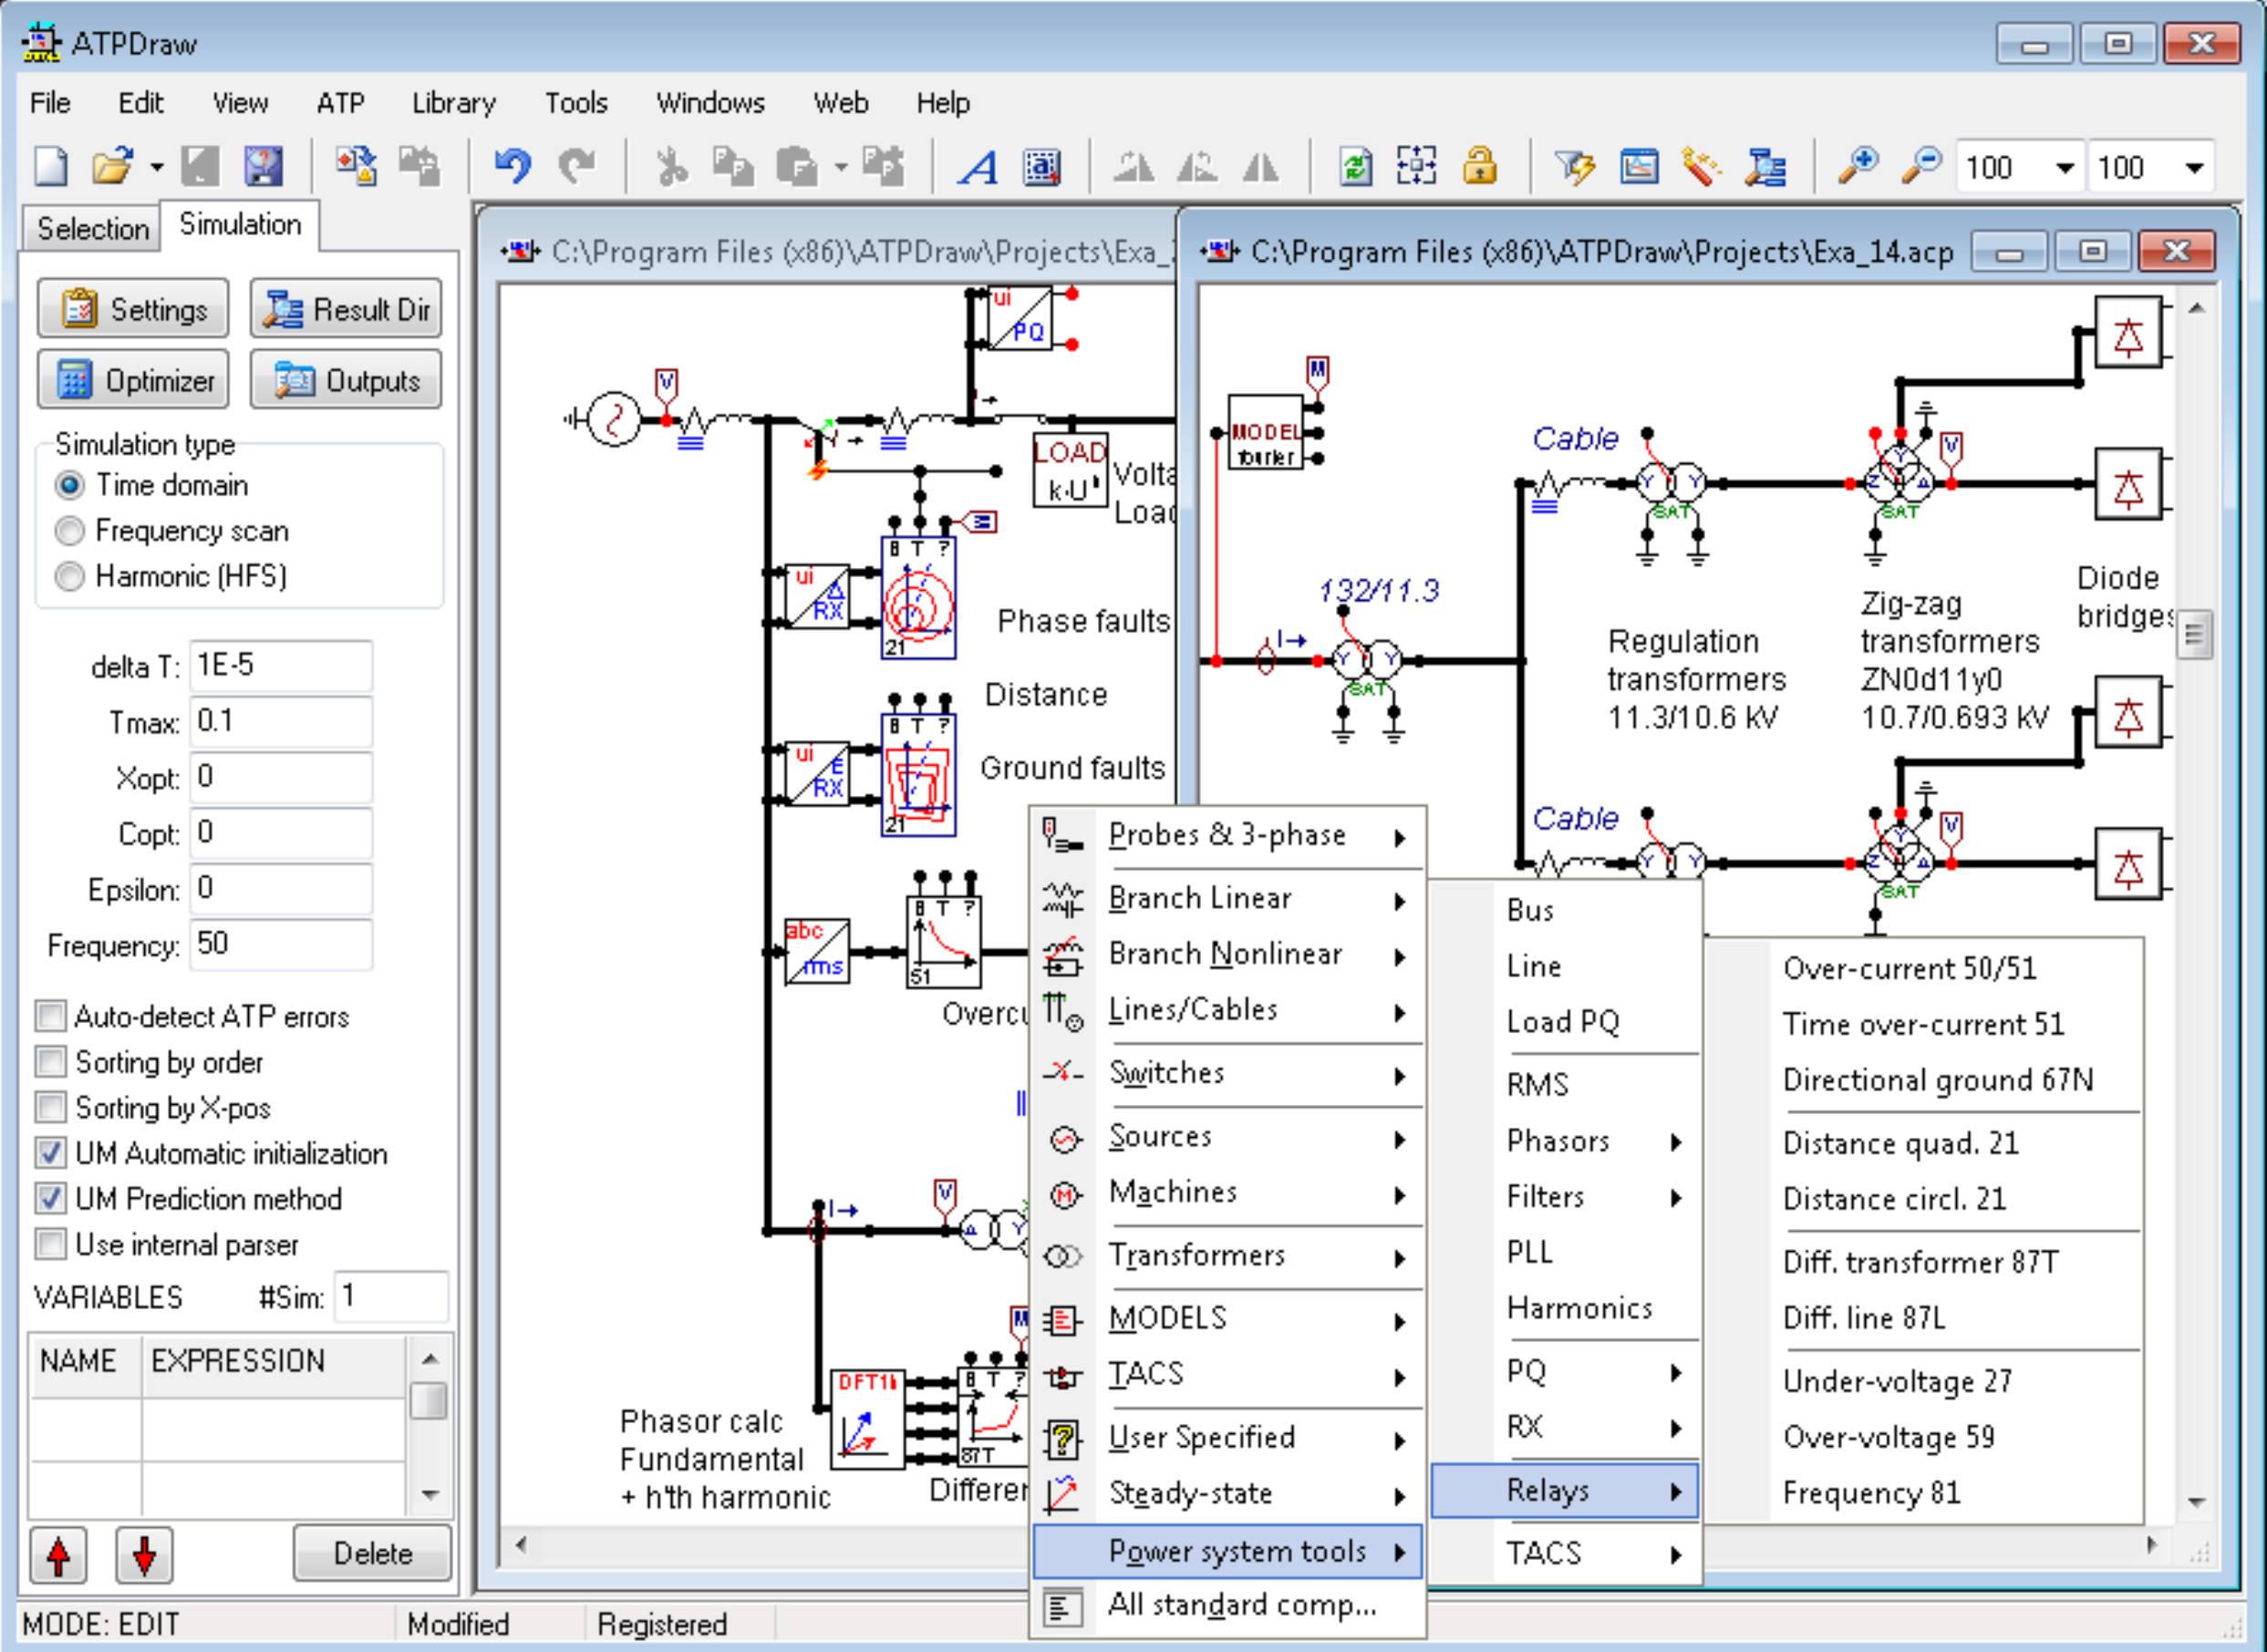
\includegraphics[width=0.8\textwidth]{img/atpdraw.png}
   \caption{ATPDraw}
   \label{atpdraw}
\end{figure}
\cite{atpsiteim}

ATP supports a wide variety of nonlinear components, switches, transformers and even support for the creation of customised elements. It can be used for time and frequency domain studies, lightning studies, electrical machines, control systems and power electronics projects.

\subsection{EMTP-RV}

EMTP-RV \cite{emtprv} is mostly written in C and C++. It was released on the market a few years after ATP. It is also a closed-source software, and it has a paid license. It is possible to obtain a free trial for a few days. It also comes with a sophisticated GUI, advanced machine models, transformer models which include magnetic core saturation and hysteresis, extensive library of control devices and functions and more.

\begin{figure}[H]
   \centering
   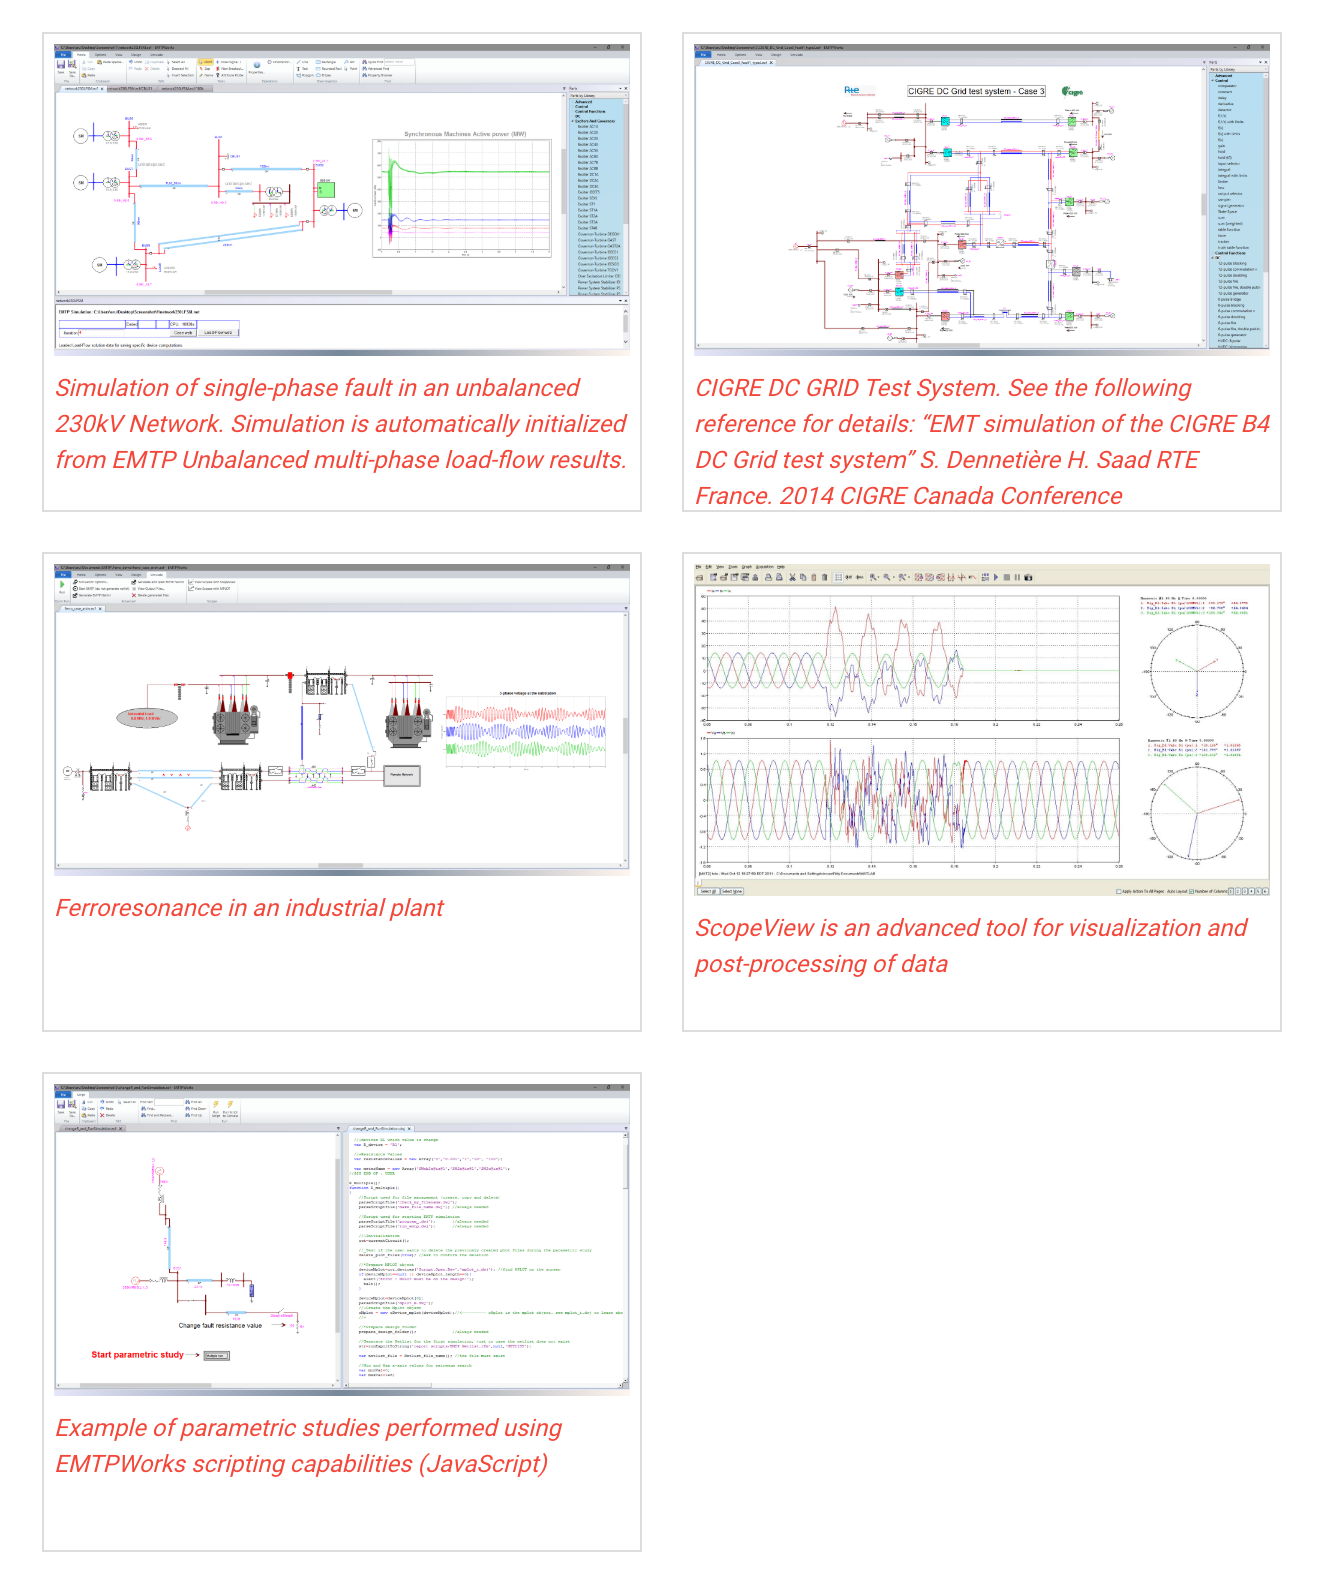
\includegraphics[width=0.8\textwidth]{img/emtp.png}
   \caption{EMTP}
   \label{emtp}
\end{figure}

EMTP implements, among other optimisations, the Critical Damping Adjustment (CDA) algorithm. "The CDA procedure eliminates the numerical oscillations that can occur in transients simulations that use the trapezoidal rule of integration"\cite{lin1990implementation}.

\section{Academic (didactic) software} \label{etr:academ}

Commercial versions are suitable for production projects, but for the learning process of undergraduate and graduate students, they might not be ideal, since their source code is often unavailable. Building a didactic prototype helps to understand the ideas behind the algorithms, possible optimisations and problems (numerical oscillations, errors, processing times). It also provides the students with a better understanding of the model and of the approach of nodal analysis method.

\subsection{ETR-P Matlab} \label{etr:thta}

Educational tool developed by a joint work from UNIFEI and UBC, this simplified Matlab/Octave version of an electromagnetic transient analysis program reads the user input from a file (in a similar format as ATP's cards) and executes the simulation. It can plot charts and it offers support to Transmission Lines, Switches and other nonlinear elements. Single-phase analysis only.

This academic project implements the CDA algorithm, as well as an equivalent technique  named by the authors of \cite{thta2015bonatto} as \textbf{"THTA"} - Trapezoidal History Term Averaging.

This project does not have an official name; the students refer to it simply as "THTA", but the nomenclature may lead to misinterpretation of what is the academic tool and what is, in fact, the Trapezoidal History Term Averaging optimisation. For this particular reason, this work refers to UNIFEI's implementation as \textbf{ETR-P} (Electromagnetic Transient Program).

ETR-P's source code is open, and it is possible to find it on Github \cite{thtaoctave}. It is not actively maintained and the code is purely procedural and imperative. It is restricted to the Matlab/Octave environment.

\subsection{ETR-Py - Python} \label{etr:pythta}

Inspired by ETRP-P, ETR-Py \cite{tavante2018open} implements a subset of features from ETR-P using the Python Language, this time using Object Oriented programming, classes, modules and popular libraries such as NumPy and SciPy. The code is also available at Github - \cite{pythta}. The features for chart plotting, Transmission Lines and Switches are not implemented yet.

When this Python version was proposed, it used to be called "PyTHTA". Once again, to avoid misunderstandings with the term "THTA", this work replaces the former name with \textbf{ETR-Py}.


\subsection{Comparison of the software alternatives}

Up to this point, only imperative code has been used to build a program to run an electromagnetic transient analysis simulation. There are other programming paradigms, and this work adopts one of them (\textbf{Functional Programming}) to create a new version of ETR-P using an utterly distinct programming style. The elaboration of this other program, named \textbf{Haskell ETR-P}, will make a robust comparison between advantages and disadvantages of each programming style possible. The code is also be open source and it is already on Github \cite{thtahs}.

The Haskell version of ETR-P aims to provide a solution where students can focus on the algorithm itself, and not on the "language plumbing" (particularities of a programming language that are required to make a program work properly but demand time and expertise to get it right). The existing academic versions mentioned at \ref{etr:thta} and even the more recent \ref{etr:pythta} are subjected to the existing problems of the imperative programming paradigm. The new approach with functional programming may help the students to use more time thinking about the algorithm and new ways to improve it.







\cleardoublepage

\chapter{ Functional Programming }
\label{fp}

Functional programming is not an entirely new concept. The nomenclature was solidified in the 1970's by J. Backus \cite{backus1978can}. In his work \cite{hughes1989functional} (published in 1990), J. Hughes summarizes the main benefits of this style by comparing pieces of code in Miranda (a functional language) with structural code. The present work will follow a similar approach. The upcoming sections will introduce and compare the main tools of functional programming. In order to fully understand the ideas, it is necessary to put aside the previous knowledge of the imperative style.

\blockquote[\cite{hughes1989functional}]{
Functional programming is so-called because its fundamental operation is
the application of functions to arguments. A main program itself is written as
a function that receives the program's input as its argument and delivers the
program's output as its result. Typically the main function is defined in terms of
other functions
} 

In other words, "the primary role of the programmer is to construct a function to solve a given problem" \cite{birdwadler} and "the primary role of the computer is to act as an evaluator or calculator".


There are many other languages labelled as \textit{functional} languages. Besides Haskell and Miranda, it is possible to mention SML, Hope and, more recently, Scala and Clojure. There are also languages which are popular among the imperative style, but also support some aspects of functional programming. This is the case of Javascript and Python. 

Some functional languages are considered to be "pure": "A language is purely functional if (i) it includes every simply typed $\lambda$-calculus term, and (ii) its call-by-name, call-by-need, and call-by-value implementations are equivalent (modulo divergence and errors)"\cite{sabry1998}. Nevertheless, this definition is not strict. In the group of "purely functional languages", it is possible to cite Haskell and SML.

Even if the definition of "purely function" is not well established, some other topics are well-agreed among the academic community when it comes to characteristics of the functional programming paradigm. They will be listed in the upcoming sections, following the summary proposed by \cite{thompson1991type}.

\section{First class functions}
Passing functions as arguments to other functions or returning functions as the result of an operation are perfectly valid steps in functional programming. Functions are interpreted with the same connotation of mathematical functions. That means it is conceivable to have several definitions for the same function:

\begin{subequations}
\begin{equation}
    f(x) = x + x
\end{equation}
\begin{equation}
    f(x) = 2x
\end{equation}
\end{subequations}

Listing \ref{lst:mainfnlit} shows an example of a simple function in a functional language.

\begin{lstlisting}[language=Haskell, numbers=left, caption={A simple function in a functional language}, captionpos=b, label={lst:mainfnlit}]
double x = x+x
\end{lstlisting}

The $ = $ operator is not binding any variable; it is actually performing the same mathematical function one finds when declaring a function. In languages like C++ or Python, it is reasonable to have a code like the following:

\begin{lstlisting}[language=Python, numbers=left, caption={Mutable references}, captionpos=b, label={lst:pythonlit1}]
a = 1
a = a + 10
\end{lstlisting}

The code on \cref{lst:pythonlit1} changes the value of the variable \lstinline!a! from 1 to 11. Such a concept is not allowed in a functional language. The \lstinline!=! operator attaches some value to a variable, and in a functional setting, it becomes immutable. A \textbf{value} is a fully simplified expression. Every time a new binding occurs, a new environment for the bound variables is created. A \textbf{function} corresponds in some sense to the methods in C++ or Python, but it also holds the mathematical foundation mentioned earlier. Analysing the \cref{lst:pythonlit1} under mathematical terms would lead to an inconsistency. 



It is also feasible to vary the body of the function according to the domain (or, interpreting it as functional programming, the input parameters) \ref{fp:domainim}.

\begin{subequations}\label{fp:domainim}
\begin{equation}
    f(x) = x, x \geq 0
\end{equation}
\begin{equation}
    f(x) = -x, x < 0
\end{equation}
\end{subequations}


It is possible to reproduce the exact same structure in functional programming by using \textbf{pattern matching}. In the main application of this work, for example, it is necessary to calculate an integer value (\lstinline!thtactl!) control for determining the final result of a current vector (in the Haskell ETR-P implementation). Simplifying the process to make the usage of pattern matching more explicit, imagine the following scenario:

\begin{lstlisting}[language=Haskell, numbers=left, caption={Pattern matching with guards. This does not correspond to the original implementation}, captionpos=b, label={lst:letexprsimplified1}]
thtaControl :: Int -> [Float]
thtaControl thtactl 
  | thtactl <= 0 = [0.0, 0.0]
  | thtactl < 3 = [1.0, 1.0]
  | otherwise = [2.0, 2.0]
\end{lstlisting}

The \lstinline![Float]! represents a list of Float numbers. In the code at \cref{lst:letexprsimplified1}, \lstinline!thtactl! is the input argument of the \lstinline!thataControl! function. Depending on its value, the behaviour of the function changes. This structure avoids the confusion of nested \lstinline!if/else! blocks.

\section{Strong type system}

It is possible to organise values in collections called \textbf{types}. There are \textbf{primitive} or \textbf{base} types (boolean, integer, float, double, etc.), and \textbf{compound} or \textbf{derived} types, whose values are build from other types (basic or compound) \cite{birdwadler}. A function is called with arguments and produces a value. When invoking a certain function (think of it as an operation), it is necessary to guarantee the call with the appropriate types of parameters. For example, calling the function \lstinline!add! with characters might not be a valid operation. The languages have mechanisms to check the validity of these types. One way to perform this \textbf{type check} is to have a compiler that captures mismatched data.

No runtime errors arise from type mismatches. This behaviour originates the label 'strong': "the domain and codomain of each function is either stated in or inferable from the program text, and there is a syntactic discipline which prevents a function from being applied to an inappropriate argument" \cite{turner1995elementary}.

\section{Polymorphic types}

Functions also have a type. For example, the \cref{lst:letexprsimplified1} has type \lstinline!(Int -> [Float])!, because it receives an integer and returns a list of float numbers. In some languages, it would be possible to generalise these types. Both integers and floats are numbers, allowing the programmer to determine that the type of the function could also be \lstinline!(Num -> [Num])!. The study of polymorphic types has several topics, but it is reasonable to think about when it is important to have generalisations. For example, to create a function that measures the \lstinline!length! of a list, it would be possible to consider the type \lstinline!([Int] -> Int)!. But then the function \lstinline!length! would be restricted to lists of \lstinline!Int! only, which is not ideal. It is feasible to generalise the domain of the function \lstinline!length! to a \textbf{Polymorphic type}: \lstinline!([a] -> Int)!.

\section{Algebraic types}


When developing a function, it is necessary to think of its return type, the type of its parameters and its body. For example, to build a \lstinline!simulation! function for Haskell ETR-P, the input would be a list of components. For the output, a Vector \lstinline!I! together with a Matrix \lstinline!V! would be the expected:

\begin{lstlisting}[language=Haskell, numbers=left, caption={Haskell ETR-P simulation function}, captionpos=b, label={lst:mainfnlit}]
thtaSimulation :: [ComponentData] -> (Vector Double, Matrix Double)
\end{lstlisting}

The \lstinline![]! denotes a list, as mentioned previously. A List can have any length, but all its elements must have the same type - that is why the type declaration consists of \lstinline![ComponentData]!, making it explicit it will be a list of ComponentData. Another structure that requires attention is the \textbf{Tuple} - they support different types in the same structure - for example, \lstinline!(Vector Double, Matrix Double)! holds a Vector and a Matrix.

A function is a value: it will be type-checked and evaluated. Just like in C++ or Python, a function can call itself, being labelled as a \textbf{recursive function}. It must contain a base case (which will indicate when to stop the process) and a recursive case (which will propagate the recursive call). 

Another crucial concept are \lstinline!let! expressions. They allow the creation of local bindings, often required by recursive function calls. See \cref{lst:letexpr1}.

\begin{lstlisting}[language=Haskell, numbers=left, caption={let expression}, captionpos=b, label={lst:letexpr1}]
diagonalUpdate :: Int -> Matrix Double -> Double -> Matrix Double
diagonalUpdate d buffer gkmHead =
  let 
      updated = (Matrix.getElem d d buffer) + gkmHead
  in  
      Matrix.setElem updated (d, d) buffer
\end{lstlisting}

The \lstinline!let! expression holds the local binding of \lstinline!updated!, which computes an intermediate value to be used at the function call triggered after the \lstinline!in! keyword. \lstinline!updated! cannot be used outside of the \lstinline!let! block.

For most of the applications, the basic types (Integer, Double, Float, Boolean, etc) in the standard library are not enough to express the goals and operations of the program. The same way one can define classes in object oriented programming, it is also possible to define custom types in functional languages. It is reasonable to aggregate several \textbf{fields} in a \textbf{Record} just as in \cref{lst:record1}.

\begin{lstlisting}[language=Haskell, numbers=left, caption={Record}, captionpos=b, label={lst:record1}]
{first = "Hanneli", last = "Tavante", course="EE"} 
\end{lstlisting}

A more structured idea than a record originates a \textbf{Datatype} as seen in \cref{lst:datatype}

\begin{lstlisting}[language=Haskell, numbers=left, caption={ComponentData datatype}, captionpos=b, label={lst:datatype}]
data ComponentData = 
  ComponentData { 
    componentType :: ComponentType,
    nodeK :: Int,
    nodeM :: Int,
    magnitude :: Double,
    param1 :: Double,
    param2 :: Double,
    plot :: Int
     }

data ComponentType = Resistor | Capacitor | Inductor | EAC | EDC
\end{lstlisting}

The custom \lstinline!ComponentData! carries several fields: componentType (whose type is also a custom type), nodeK, nodeM, magnitude, param1, param2 and plot.

Another example of DataType is the \lstinline!ComponentType!. The constructors do not have any parameters (Resistor, Capacitor, etc). To obtain the component type of a component data, a set of \lstinline!if/else! blocks would be required (when thinking according to the imperative programming style). In a functional setting, there is \textbf{Pattern Matching}. The code in \cref{lst:pmcase11} provides another example of this feature, this time using a \textbf{case} expression:

\begin{lstlisting}[language=Haskell, numbers=left, caption={Pattern matching example with case}, captionpos=b, label={lst:pmcase11}]
condutance :: ComponentData -> Double -> Double
condutance component dt =
  case componentType component of
    Resistor -> 1.0 / (magnitude component)
    Capacitor -> (magnitude component) * 0.000001 * 2 / dt
    Inductor -> dt / (2 * 0.001 * (magnitude component))
    _ -> 0.0
\end{lstlisting}

It is also possible to work with pattern matching when declaring the function's body as seen in \cref{lst:pmfn}:


\begin{lstlisting}[language=Haskell, numbers=left, caption={Pattern matching in functions}, captionpos=b, label={lst:pmfn}]
buildIVector :: [ComponentData] -> Vector Double -> Vector Double -> Vector Double
buildIVector [] _ iVector = iVector
buildIVector (component:cs) ih iVector =
-- recursive case omitted
\end{lstlisting}

\lstinline!buildIVector! can be pattern matched against its own parameters. Its behaviour changes when it receives an empty list (meaning the end of the recursion) or when it receives a non-empty list, denoted by \lstinline!(component:cs)!. The underscore means the value does not have any influence on that pattern matching format.


\section{Modularity}

There are systems of modules which can be attached to projects, making the development of larger systems easier and more organised. For the developed Haskell ETR-P, for example, a few modules were required to build the project as shown in \cref{lst:moduleshs}.


\begin{lstlisting}[language=Haskell, numbers=left, caption={Modules}, captionpos=b, label={lst:moduleshs}]
-- vector
import Data.Vector (Vector)
import qualified Data.Vector as Vector

-- Matrix
import Data.Matrix (Matrix)
import qualified Data.Matrix as Matrix

-- HMatrix
import qualified Numeric.LinearAlgebra.Data as HMatrix
import qualified Numeric.LinearAlgebra.HMatrix as HMatrix

-- bytestring
import Data.ByteString.Lazy (ByteString)
import qualified Data.ByteString.Lazy as ByteString
\end{lstlisting}

In \cref{lst:moduleshs}, it is possible to find the Vector, Matrix, HMatrix and ByteString modules. It is plausible to import them to the main project assigning an alias. For example, \lstinline!import qualified Data.Matrix as Matrix! adds the alias \lstinline!Matrix! to the module \lstinline!Data.Matrix!.

\section{Fucntional Programming - summary}

"Functional programming can be contrasted with imperative programming either in a negative or a positive sense"\cite{harrison1997introduction}. Combining the "pros" and "cons" listed at \cite{harrison1997introduction} and at \cite{michaelson2011introduction}, it was possible to built the table \ref{tab:funcvsimperative}, which aims to be impartial and summarise an objective and concise comparison of the main differences between these two paradigms:

% Please add the following required packages to your document preamble:
% \usepackage{graphicx}
% \usepackage[table,xcdraw]{xcolor}
% If you use beamer only pass "xcolor=table" option, i.e. \documentclass[xcolor=table]{beamer}
\begin{table}[H]
\resizebox{\textwidth}{!}{%
\begin{tabular}{c
>{\columncolor[HTML]{FFCE93}}l 
>{\columncolor[HTML]{DAE8FC}}l }
\multicolumn{1}{l}{}                                                   & \multicolumn{1}{c}{\cellcolor[HTML]{FFCE93}\textbf{Imperative Paradigm}}                                                                       & \multicolumn{1}{c}{\cellcolor[HTML]{DAE8FC}\textbf{Functional Paradigm}}                                                                            \\ \hline
\multicolumn{1}{|c|}{\cellcolor[HTML]{EFEFEF}\textbf{Main component}}  & \multicolumn{1}{l|}{\cellcolor[HTML]{FFCE93}Statements}                                                                                        & \multicolumn{1}{l|}{\cellcolor[HTML]{DAE8FC}\begin{tabular}[c]{@{}l@{}}Functions \\ (can be treated as values)\end{tabular}}                        \\ \hline
\multicolumn{1}{|c|}{\cellcolor[HTML]{EFEFEF}\textbf{Assignments}}     & \multicolumn{1}{l|}{\cellcolor[HTML]{FFCE93}\begin{tabular}[c]{@{}l@{}}The same name \\ may be associated with \\ the same value\end{tabular}} & \multicolumn{1}{l|}{\cellcolor[HTML]{DAE8FC}\begin{tabular}[c]{@{}l@{}}No assignments. \\ A name is only \\ associated with one value\end{tabular}} \\ \hline
\multicolumn{1}{|c|}{\cellcolor[HTML]{EFEFEF}\textbf{Execution order}} & \multicolumn{1}{l|}{\cellcolor[HTML]{FFCE93}Crucial importance}                                                                                & \multicolumn{1}{l|}{\cellcolor[HTML]{DAE8FC}Not very important}                                                                                     \\ \hline
\multicolumn{1}{|c|}{\cellcolor[HTML]{EFEFEF}\textbf{Mutability}}      & \multicolumn{1}{l|}{\cellcolor[HTML]{FFCE93}\begin{tabular}[c]{@{}l@{}}Yes, most of the time the \\ structures are mutable\end{tabular}}       & \multicolumn{1}{l|}{\cellcolor[HTML]{DAE8FC}Usually not present}                                                                                    \\ \hline
\multicolumn{1}{|c|}{\cellcolor[HTML]{EFEFEF}\textbf{State changes}}   & \multicolumn{1}{l|}{\cellcolor[HTML]{FFCE93}Essential building block}                                                                          & \multicolumn{1}{l|}{\cellcolor[HTML]{DAE8FC}No state}                                                                                               \\ \hline
\multicolumn{1}{|c|}{\cellcolor[HTML]{EFEFEF}\textbf{Flow control}}    & \multicolumn{1}{l|}{\cellcolor[HTML]{FFCE93}\begin{tabular}[c]{@{}l@{}}Loops, if/else, \\ exceptions\end{tabular}}                             & \multicolumn{1}{l|}{\cellcolor[HTML]{DAE8FC}\begin{tabular}[c]{@{}l@{}}Recursion, \\ pattern matching, \\ IO\end{tabular}}                          \\ \hline
\end{tabular}%
}
\caption{Comparison: Imperative and Functional paradigms}
\label{tab:funcvsimperative}
\end{table}


% \section{Other concepts}
% [TODO]
% Recursion and induction
% recursive types














\cleardoublepage

\chapter{Haskell}
\label{haskell}

Haskell is a functional language developed in the 1990s. Designed to be lazy, pure and to support type classes \cite{hudak2007history}, the language has been evolving since its creation. This chapter will provide examples of some of the functional programming concepts introduced in Chapter \ref{fp} using the Haskell language. This chapter is not a "Haskell Tutorial"; its primary goal is to present the concepts of functional programming that will be used in the practical section and, therefore, will be one of the central objects of study of this work. The fundamental ideas of the next section come from \cite{hutton2016programming}, and from \cite{fp101em} (course at TU Delft); those are also good references to get started into Haskell programming.

The development of the Haskell language started in 1987 \cite{hudak2007history}, but its foundations started a few decades before, with Alonzo's Church Lambda Calculus. In the 1970s, John Backus inaugurated the term \textit{Functional style} in his work \cite{backus1978can}, motivating a meeting of programming language researches ten years later. This group officially started the works on the Haskell language.

The principal features of the Haskell language \cite{hutton2016programming} are listed below:

\begin{itemize}\label{lsthbenefits}
\item Concise programs - Haskell's syntax is designed to be compressed and to have just a few keywords. \textit{List Comprehensions}, for example, are a concise way to navigate on a list, create new ones, filter elements or transform the existing ones. No need for explicit loops (like \lstinline!while!) or nested if/else blocks.
\item Type system - Haskell's type system helps programmers to detect incompatibility errors at compile time (the functions often require the expected input and output types). Haskell supports polymorphism and overloading, providing the developers with a wide range of features.
\item Recursive functions - One and probably the most important way to navigate through a collection of elements is using \textbf{recursion}. To determine when to stop or to continue, recursion can be combined with \textbf{pattern matching}.
\item Higher-order functions - Functions can receive other functions as arguments, as well as return them as values. A \textbf{higher order function} abstracts the behaviour of a group of functions, wrapping it up in another function.
\item Effectful functions - A function is called \textbf{pure} when it produces the same output given the same inputs, without any interference. In some circumstances, there may be \textit{side effects}, causing unexpected outputs. Operations that involve files are a good example of impurity. If a function requires a file, it may or may not be present, causing the function to have multiple outputs for the same inputs. It will be an \textbf{impure} function. Haskell provides mechanisms to deal with this impurity scenario: \textit{monads} and \textit{applicatives}.
\item Lazy evaluation - In Haskell, a computation is not performed until it is required by another function. This mechanism avoids unnecessary computations and allows the usage of infinite structures, such as infinite lists.
\item Equational reasoning - Combined with induction, it can be used to transform, execute and demonstrate properties of Haskell programs.
\end{itemize}


\section{Function and Types in Haskell}

Recall that one of the aspects of functional programming is having a style closer to a mathematical representation. In this context, \lstinline[language=haskell]{f x} in the Haskell language corresponds to the mathematical function application $ f(x) $. In other words, an empty, blank space represents a function application.

\subsection{Basic types}

Another topic that arises in functional languages are \textbf{types}: they are a collection of related values, as seen in \cref{lst:typesdecla}.

\begin{lstlisting}[language=Haskell, label={lst:typesdecla}, caption={Types for variables and expressions}, captionpos=b]
v::T -- v has type T
e::T -- The evaluation of the expression e will produce a value of type T
\end{lstlisting}

In Haskell, every expression must have a type. For this language, it is possible to either manually define the types or to have them inferred using the \textbf{type inference} process. This step happens before the proper evaluation, so if there is anything that does not match the possible type (for example, adding a string with an integer), the code will not compile. Making types explicit when writing functions is a good practice in Haskell. Mathematically speaking, this is shown in \cref{fig:proof1}:

\begin{figure}[H]
\caption{Transient Analysis - Example Circuit}
\label{fig:proof1}
\begin{prooftree}
  \AxiomC{$f::A \rightarrow B $}
  \AxiomC{$ e::A $}
  \BinaryInfC{$ f e::B $}
\end{prooftree}
\end{figure}

Figure \ref{fig:proof1} states that if there is a function \textbf{f} that maps an argument of type \textbf{A} to a result of type \textbf{B} and \textbf{e} is an expression of type \textbf{A}, the application of the function \textbf{f} will have the type \textbf{B}.

Haskell programs are labelled as \textit{type safe} because the compiler guarantees the absence of type errors during run time. One downside about this feature is that sometimes a valid expression may be misinterpreted during the type inference process, causing it to reject a correct expression.

Some examples of built-in types in Haskell are Int, Float, Double. There are also more sophisticated built-in types in Haskell - Lists, collections of elements of the same types; and Tuples, finite sequences of components, which can be of different types. An example can be found in \cref{lst:examplesbuiltintypes}.

\begin{lstlisting}[language=Haskell, label={lst:examplesbuiltintypes}, caption={Lists and Tuples}, captionpos=b]
[1,2,3] -- A List of Integers
("Hanneli","UNIFEI",2019,True) -- A Tuple of arity four (four elements)
\end{lstlisting}

Conceptually, Lists require a specification of the type they will convey. It is reasonable to have lists of Integers, Floats and Strings, for examples. Generalising, there is the type \lstinline[language=haskell]{List a}, where \textbf{a} is a variable to indicate a type. A type (in this case, \textbf{List}) that contains one or more type variables (in this case, \textbf{a}), is a \textbf{polymorphic type}.


A \textbf{List} like [1,2,3] is equivalent to \lstinline[language=haskell]{(1:(2:(3:[])))}. From this alternative representation it is possible to see that lists are recursively compounded. Initially, there is the empty list \lstinline[language=haskell]{[]}, and then 3, then 2, then 1 are appended. In functional languages, recursion is very important to compose several data structures. Recursion is also the basic looping mechanism. In Java or C++, it is common to find a \textbf{for} loop accessing items of collections by indexes. In contrast, Haskell relies on recursion to perform operations across lists. For example, multiplication can be defined as a recursive sum as shown in \cref{lst:recursivesumexample}.


\begin{lstlisting}[language=Haskell, label={lst:recursivesumexample}, caption={Recursion}, captionpos=b]
mult _ 0 = 0 -- Base case
mult n m = (mult n (m - 1)) + n -- Recursive call
\end{lstlisting}


Given that a function can receive other functions as arguments and return other functions, a function is itself a type. That means functions receiving multiple parameters can be rewritten as functions that receive a single parameter and return another function. This is called \textbf{currying}. For example, when declaring a function \lstinline!adds! to add two integers, the function type can be defined as something that receives two integers and returns another integer ( \lstinline!adds :: Int -> Int -> Int! ) or as a function that takes only one integer and returns another function that takes the second integer and returns the result: \lstinline!adds :: Int -> (Int -> Int)!. In the previous example, the parentheses are optional, since the \lstinline!->! (named 'arrow function') is interpreted as right-associative. So \lstinline!Int -> Int -> Int -> Int! is the same as \lstinline!Int -> (Int -> (Int -> Int))!.

However, function application (denoted by a simple space character \lstinline!" "!) associates to the left. So \lstinline!adds x y z! means \lstinline!((adds x) y) z!.

In Haskell, the concept of \textit{class} differs from the idea of the object-oriented languages. A class is a collection of types that supports overloaded operations (\textit{methods}). For example, \textit{Equality} is a class that contains a method \lstinline!(==)! under the type signature of \lstinline!(==) :: a -> a -> Bool!, that determines if an element of the collection of types \lstinline!a! is equal to another of the same type, a Bool result must be returned. Ordering (\lstinline!ord!), \lstinline!Show!, \lstinline!Read!, Numerical (\lstinline!Num!) and \lstinline!Fractional! are other examples of Haskell classes.


\subsection{Function structure and resources}\label{haskell:fnstr}

Haskell supports \lstinline!if/else! blocks (example: \lstinline!if n == 0 then 0 else 1!), but it is much more common to use \textit{guard} expressions (see \cref{lst:letexprsimplified1}) or \textit{pattern matching} (see \cref{lst:pmcase}):

\begin{lstlisting}[language=Haskell, numbers=left, caption={Pattern matching with case}, captionpos=b, label={lst:pmcase}]
condutance :: ComponentData -> Double -> Double
condutance component dt =
  case componentType component of
    Resistor -> 1.0 / (magnitude component)
    Capacitor -> (magnitude component) * 0.000001 * 2 / dt
    Inductor -> dt / (2 * 0.001 * (magnitude component))
    _ -> 0.0
\end{lstlisting}

It is possible to pattern match against Lists, Tuples and other types.

It is feasible to define auxiliary, nameless functions. They are called \textbf{lambda} expressions and a similar concept is present in some object-oriented languages such as Python. In \cref{lst:lambdafunction}, there is a lambda expression right after \lstinline!map!. This anonymous function specifies one should be added to the value of each component of a collection. \lstinline!\! indicates the declaration of a lambda expression. The name 'lambda' expression originates from $\lambda$-Calculus (visit \cref{sec:lc} for more information).

\begin{lstlisting}[language=Haskell, numbers=left, caption={Lambda functions}, captionpos=b, label={lst:lambdafunction}]
map (\r -> (r + 1)) [1, 2, 3]
\end{lstlisting}

\lstinline!map! applies another function to each element of a list. For example, to add 2 to all the elements of \lstinline![1, 2, 3]!, one can invoke the \lstinline!map! function as in \lstinline!map (+2) [1, 2, 3]!. 

\subsection{Higher order functions}

Higher-order functions allow common programming patterns to be wrapped in a function. To build the intuition on this topic, it is reasonable to sketch an example with the \lstinline!fold! function. "Folding" a list means to compress it following a certain operation. For example, \lstinline!foldl (+) 0 [1, 2, 3]! returns 6; the 0 is the initial buffer. $+$ is the operation, and $0 + 1 + 2 +3$ is the result of \lstinline!fold!. Alternatively, \lstinline!foldl (+) 1 [1, 2, 3]! returns 7, because the initial accumulator is 1.

"\lstinline!fold! takes an 'initial answer' \lstinline!acc! and uses [a function] \lstinline!f! to 'combine' \lstinline!acc! and the first element of the list, using this as the new 'initial answer' for 'folding' over the rest of the list"\cite{plcoursera}. A collection can be folded to the left with \lstinline!foldl! or to the right with \lstinline!foldr!. The \cref{lst:foldl} describes the implementation of a left fold, named as \lstinline!foldl2!, since \lstinline!foldl! is the name of the funciton in the standard implementation of the Haskell language.

\begin{lstlisting}[language=Haskell, numbers=left, caption={fold left}, captionpos=b, label={lst:foldl}]
foldl2 f v [] = v
foldl2 f v (x:xs) = foldl2 f (f v x) xs
\end{lstlisting}

The type signature of \lstinline!foldl! is given by \cref{lst:foldltypesig}:

\begin{lstlisting}[language=Haskell, numbers=left, caption={fold left type signature}, captionpos=b, label={lst:foldltypesig}]
foldl :: (a -> b -> a) -> a -> [b] -> a
\end{lstlisting}

Functions can be composed the same way they are composed in mathematics. The higher-order composition function (denoted by the operator \lstinline! . !) allows the function composition $ f \circ g $ with the syntax \lstinline!f . g! .

\subsection{Composite types}

It is possible to define custom types in Haskell by using the keyword \textbf{data}. The \cref{lst:haskellex1ch4} is an example of a new data called Shape, which has two possible constructions: it can be a Circle or a Rectangle.

\begin{lstlisting}[language=Haskell, label=getinfo, caption={Custom types}, captionpos=b, label={lst:haskellex1ch4}]
data Shape = Circle Float | Rectangle Float Float

square::Float -> Shape
square n = Rectangle n n 

\end{lstlisting} 

\textbf{Rectangle} and \textbf{Circle} are constructor functions. They exist for building pieces of data, but they do not carry the defining equations. The logic to build the actual rectangle is in the function \textbf{square}. This is consistent with the principles of functional programming: the data is isolated, and the basic method of computation to build anything is the application of functions.

The keyword \textit{type} adds an alias to existing types. For example, \lstinline!type String = [Char]!, implies that \lstinline!String! is just a List of \lstinline!Char!. Type declarations can be parameterised by other types. For example, \lstinline!type Pair a = (a, a)!.

\section{Impure functions}
\label{sideeffects}

One of the key ideas in functional programming is the concept of \textit{pure functions}. They have no side effects (they do not mutate any state of the program or change non-local variables). These functions also return the same value given the same input arguments, just as a regular mathematical function.

However, I/O operations can have side effects. For example, opening a file may succeed or may throw an error, either because the file does not exist or because it is corrupted. Note that this problem has nothing to do with manipulating the information on a file; it is an external problem. Realistically, it is only possible to have a code that expects the possibility of a side effect. Languages like Java deal with this scenario by throwing run time exceptions. 

Haskell represents impurity with the \lstinline!IO! type. Expressions of this type are named as \textit{actions}. 

The use case presented in this work requires, from the very first beginning, an action that will generate side effects - reading CSV files with the input data. A function to read and parse the data can have side effects when (a) the file is not in the specified directory; (b) the file does not exist; (c) the file is empty; (d) the file is corrupted. The type of a parsing function must incorporate the possibility of these side effects, and for that matter, two elements are required:
\begin{enumerate}
  \item an action to change the context from pure to impure (\lstinline!return! function in \cref{lst:donotation});
  \item a sequencing operator to apply the parser and call the result, then reapply the parser, get the result and repeat the process until the end of the file is reached. A sequence of actions can be chained with the \lstinline!do! notation as seen in \cref{lst:donotation}.
\end{enumerate}


\begin{lstlisting}[language=Haskell, caption={do notation; Note: this is just a didactic draft example.}, captionpos=b, label={lst:donotation}]
do
  eitherSimulation <- decodeSimulationFromFile "data/simulation.csv"
  componentsList <- decodeItemsFromFile "data/components.csv"
  return (eitherSimulation, componentList)
\end{lstlisting}


\section{Monads}
\label{hsmonads}

Haskell supports even more generic sets of functions - some of them can be generalised over a range of parameterised types (lists, trees, IO). For example, it is possible to generalise the idea of \lstinline!map! to other structures rather than Lists. In the reference implementation of this work, in many scenarios \lstinline!map! occurs in a \lstinline!Vector!. This generalisation is seen on \cref{lst:mapvecfnd}:

\begin{lstlisting}[language=Haskell, numbers=left, caption={map in a Vector}, captionpos=b, label={lst:mapvecfnd}]
gkm :: Vector ComponentData -> Double -> Vector Double
gkm components dt =
  Vector.map (\c -> condutance c dt) components
\end{lstlisting}

There is a class of types supporting the \lstinline!map! function - this is the \lstinline!Functor! class, with \lstinline!fmap! as the generic function that maps another function over each element of a structure \cite{hutton2016programming}.

\begin{lstlisting}[language=Haskell, numbers=left, caption={Functor class}, captionpos=b, label={lst:functorfmap}]
class Functor f where
  fmap :: (a -> b) -> f a -> f b
\end{lstlisting}

\ref{lst:mapvecfnd} is an example of a Functor. Functors work for single-element functions. It is possible to generalise the idea of Functor itself, making it support any number of parameters, as suggested in \cref{genfunctors}.

\begin{figure}[H]
   \centering
   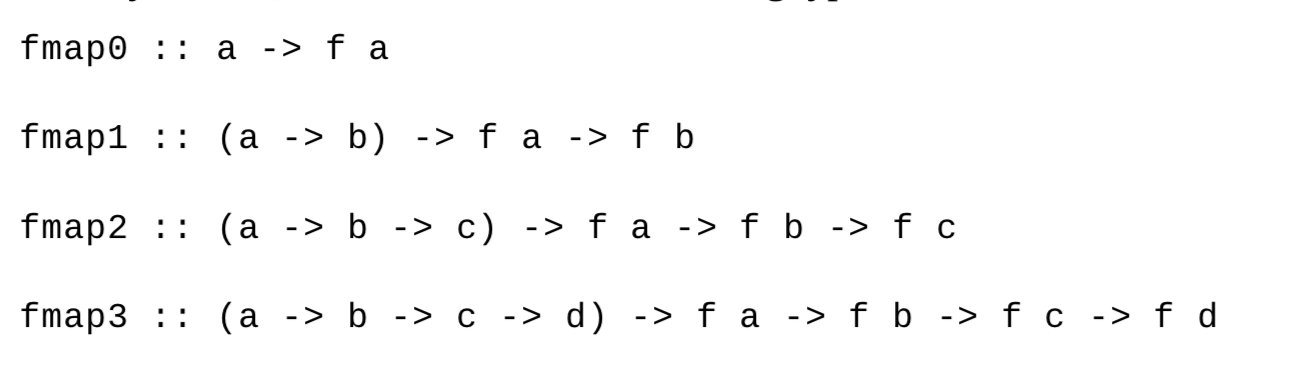
\includegraphics[width=0.9\textwidth]{img/functorapplicative.png}
   \caption{Generalising functors}
   \label{genfunctors}
\end{figure}
\cite{hutton2016programming}

Two basic functions are capable of encoding the desired generalisation. They are built using the idea of currying and are described in  \cref{lst:applicatives}:


\begin{lstlisting}[language=Haskell, numbers=left, caption={Applicatives}, captionpos=b, label={lst:applicatives}]
class Functor f=> Applicative f where
  pure :: a -> f a
  (<*>) :: f (a -> b) -> f a -> f b 
\end{lstlisting}

This pair of functions is called \textbf{Applicative Functor} (or simply \textbf{Applicatives}). Examples of its usage can also be found in the implementation of Haskell ETR-P in \cref{lst:usingapplicatives}:

\begin{lstlisting}[language=Haskell, numbers=left, caption={Using Applicatives}, captionpos=b, label={lst:usingapplicatives}]
instance FromNamedRecord ComponentData where
  parseNamedRecord m =
    ComponentData
      <$> m .: "Element Type"
      <*> m .: "Node K"
      <*> m .: "Node M"
      <*> m .: "Value"
      <*> m .: "Source param 1"
      <*> m .: "Source param 2"
      <*> m .: "Plot"

instance FromField ComponentType where
  parseField "R" =
    pure Resistor

  parseField "L" =
    pure Inductor

  parseField "C" =
    pure Capacitor

  parseField "EDC" =
    pure EDC

  parseField "EAC" =
    pure EAC

  parseField otherType =
    Other <$> parseField otherType
\end{lstlisting}


In Haskell, it is possible to encode a possibility of failure in the function's type. The \lstinline!Maybe! type wraps a success branch (named \lstinline!Just a!) or a possible failure, represented by the absence of value (represented by \lstinline!Nothing!). The \textbf{bind} operator \lstinline!>>=! takes an argument of type "a"  and a function of type \lstinline!a -> b!. Both can fail, the argument and the function. \lstinline!>>=! returns a result of type "b", which can also be a failure (encoded as a Maybe) as shown in \cref{lst:bindoperator}:


\begin{lstlisting}[language=Haskell, numbers=left, caption={The bind operator}, captionpos=b, label={lst:bindoperator}]
(>>=) :: Maybe a -> (a -> Maybe b) -> Maybe b
mx >>= f = case mx of
           Nothing -> Nothing
           Just x -> f x
\end{lstlisting}

It is also necessary to have a function that provides a connection between pure functions and actions (impure). This is the \textbf{return} function, with the signature defined in \cref{lst:returnfunc}.

\begin{lstlisting}[language=Haskell, numbers=left, caption={The return}, captionpos=b, label={lst:returnfunc}]
return :: a -> IO a
\end{lstlisting}

The \lstinline!return! function defined in \cref{lst:returnfunc} has nothing to do with the "return" statements found in languages like C.

A \textbf{Monad} arises from the combination of these two elements, \lstinline!>>=! and \lstinline!return!. A Monad is an applicative that supports both of these operations. "Every Monad is an applicative functor"\cite{lipovaca2011learn} in its generalised form, as proposed in \ref{genfunctors}. This work will not explore in detail the powerful constructions built on the monadic style. A complete example of Monad applications can be found on the work of \cite{hutton1998monadic}. The code in \cref{lst:parserex} and \cref{lst:parserexmonad} describe a Monadic parser with the two principal elements of a Monad: the \lstinline!return! and bind operator \lstinline!>>= !:

\begin{lstlisting}[language=Haskell, caption={Declaring the type Parser}, captionpos=b, label={lst:parserex}]
newtype Parser a = Parser (String -> [(a,String)])
\end{lstlisting}

\begin{lstlisting}[language=Haskell, caption={Declaring the type Parser}, captionpos=b, label={lst:parserexmonad}]
instance Monad Parser where
  return a = Parser (\cs -> [(a,cs)])
  p >>= f = Parser (\cs -> concat [parse (f a) cs' |
    (a,cs') <- parse p cs])
\end{lstlisting}

\section{Advanced Features and fields of study}

The previous sections provided the basic concepts required to understand and interpret the code in Chapter \ref{implhs}. However, the Haskell language has been evolving continuously and it has advanced topics which are also out of the scope of this work. Just to give a taste to the reader, some of the active research topics involve (but are not limited to): Deep EDSL \cite{gill2014domain}, verification of Haskell programs with type theory \cite{abel2005verifying}, constraint solving \cite{hallahan2019g2q}, Monad transformers \cite{schrijvers2016monad}, verification of Haskell programs in proof interactive theorem provers (like Coq \cite{coqurl} or Liquid Haskell \cite{liquidhaskell}, see \cite{Christiansen} and \cite{vazou2016liquid}), program synthesis in Haskell \cite{Finkbeiner}, etc.











\cleardoublepage


\chapter{ Haskell in Electromagnetic Transient Analysis - Implementation}
\label{implhs}

This chapter describes the development of the principal analysis tool for this work: a functional version of the original ETR-P software rewritten in Haskell. The upcoming sections do not follow the same order of content creation; instead, they try to build a more intuitive connection between the theory of functional programming and a practical aspect of its application when building a program for electromagnetic transient analysis. Each section methodically follows the same basic structure:

\begin{itemize}
\item Logical explanation of the electrical process
\item Haskell implementation
\item Functional programming resources
\item Comparison with the implementation in ETR-P using Matlab/Octave. Additional languages, such as Python and C++, will also be targeted for contrasting the different paradigms.
\item Improvements and future work
\end{itemize}


\section{ The goals for a Haskell version of ETR-P }
\label{haskellgoal}

The main goal of this open-source Haskell program is to compare the style differences between functional and imperative code. This version does not contain all the features supported at the original ETR-P. Its scope was limited in order to demonstrate a proof of concept. Non-linear components, switches, transmission lines are not implemented. Triangular voltage sources and external current sources were put aside for the initial implementation. RLC components, DC and sinusoidal elements are the core of this Haskell program. It is restricted to single-phase circuits.

Optimisation, performance, graphics, UI, charts and user input are popular topics in program development, but they are not the goal of this work either. This project is a comparison of programming paradigms and an analysis of the outcomes. 

Following H. W. Dommel's original proposition in \cite{dommel1969digital}, this program reads in the circuit data, creates the initial steady-state matrix equations for initialization of equivalent historic sources of digital lumped components. Then it solves the nodal equations $ [G] [V] = [I_h] $ for every time step (where $ G $ is the conductances matrix, and $ I_h $ are the historical and external current sources), obtaining the final values for nodal voltages, branch voltages and branch currents after the simulation time. Translating this goal to Haskell, it is necessary to elaborate a function with the type described in \cref{lst:mainfnsig}. It follows the functional programming principle that says "Programs in Haskell can be viewed as functions whose input is that of the problem being solved, and whose output is the desired result.[...] The behaviour of the function can be understood as [..] computation by calculation". \cite{hudak2000haskell}

\begin{lstlisting}[language=Haskell, numbers=left, caption={ETR-P Haskell goal's function}, captionpos=b, label={lst:mainfnsig}]
thtaSimulation :: Vector ComponentData -> SimulationData -> SimulationResults
\end{lstlisting}

In \cref{lst:mainfn}, the function \textbf{thtaSimulation} receives two parameters: the components representing the circuit (\textbf{Vector ComponentData}) and the simulation data (\textbf{SimulationData}). It returns a tuple with a the final current vector and the final voltage matrix, represented by the type \textbf{SimulationResults}.

In ETR-P (Matlab/Octave), there is no single function isolating this compact representation. Instead, there is a single block of code sequentially declaring the steps of the algorithm.

The following section \ref{haskellimpl} will describe data acquisition from a set of files.

\subsection{ Data input }
\label{haskellimpl}

The data describing the simulation parameters and the components of the circuit is stored in external files. This part of the code must handle the data and feed the algorithm with the collected information.  Just like the implementation of ETR-Py, this the initial circuit status will be stored in \lstinline!.csv! files. ETR-P (Matlab/Octave) uses a \lstinline!.txt! file.  

The Haskell implementation requires two different files (one for components and another for the simulation parameters). A well-formed CSV does not mix different sources of information, making it inappropriate to store the Time and other information of the simulation along with the components and nodes information. The original ETR-P and also ETR-Py handle this step improperly mixing these two sources of information in the same input file.

Listing \ref{csgetinfo1} and \cref{csgetinfo2} are examples of the input data split in two files.

\begin{lstlisting}[language=bash, label=csgetinfo1, caption={Input data file for components}, captionpos=b]
Element Type,Node K,Node M,Value,Source param 1,Source param 2,Plot
EDC,2,0,10,0,0,0 
R,2,1,10,0,0,0
L,1,0,1,0,0,0
\end{lstlisting}


\begin{lstlisting}[language=bash, label=csgetinfo2, caption={Input data file for time and simulation data}, captionpos=b]
Number of Nodes,Number of Voltages Sources,Step Size,Maximum time for simulation
2,1,0.0001,0.05
\end{lstlisting}

Listing \ref{csgetinfoorig1} shows the input file format of the original ETR-P Matlab program:

\begin{lstlisting}[language=bash, label=csgetinfoorig1, caption={Original input data file for ETR-P Matlab}, captionpos=b]
T   2   1   100E-6  50E-3    0   0   0   0   0
EDC 2   0   10      0       0   0   0   0   5
R   2   1   10      0       0   0   0   0   5
L   1   0   1       0       0   0   0   0   5
NV  1   2   0       0       0   0   0   0   0
\end{lstlisting}


Headers were also inserted on each CSV file to make their columns self-explanatory (\cref{csgetinfo1} and \cref{csgetinfo2}). These headers are taken into consideration when parsing the files in the Haskell implementation.


File operations are considered impure (details in \cref{sideeffects}), given that they can generate several unexpected behaviours to a function. Some of the possible are listed below:

\begin{enumerate}\label{impureprobl1}
  \item File path is incorrect;
  \item File is corrupted;
  \item File is in the wrong format (not a CSV);
  \item A well-formed CSV is expected to have data in all the columns, for all the rows. The file might contain missing data;
  \item File is in a different encoding (example: file contains characters from a different alphabet rather than the Latin alphabet);
\end{enumerate}

As described in \cref{sideeffects}, it will be necessary to use Haskell's specific mechanisms to deal with possible side effects. 

The first step is building a parser to take the \lstinline!.csv! file and turn it into proper types. The implementation in this work uses the library \textbf{cassava} for handling the parsing. The implementation starts with the \lstinline!components.csv! file, describing each component and their corresponding position in the circuit (see \cref{lst:csv1}).


\begin{lstlisting}[language=Haskell, numbers=left, caption={Initial implementation of CSV file parsing with cassava}, captionpos=b, label={lst:csv1}]
{-# LANGUAGE OverloadedStrings #-}
{-# LANGUAGE RecordWildCards #-}

module Main where

import qualified Data.ByteString.Lazy as BL
import qualified Data.Vector as V
-- from cassava
import Data.Csv

type ComponentData = (BL.ByteString, Int, Int, Float, Param, Param, Int)

main :: IO ()
main = do
  csvData <- BL.readFile "data/components.csv"
  let v = decode NoHeader csvData :: Either String (V.Vector ComponentData)

\end{lstlisting}

The code at \cref{lst:csv1} imports the basic modules (from lines 6 to 9), followed by a basic \textbf{type} declaration: \lstinline!ComponentData!. It matches the structure of each line of the CSV file \textit{components.csv}. \lstinline!ComponentData! is just a synonym to a tuple structure made of \lstinline!(BL.ByteString, Int, Int, Float, Param, Param, Int)!. Next, in the main body, the file is read with \lstinline!BL.readFile! and its content is decoded, ignoring the CSV header. The result of reading a file can be either a well-formed data or an error. That is why the \lstinline!Either! type is necessary: to carry either a successful output (which is called Right) or an error (wich is called Left, by convention).

Even though the code on \cref{lst:csv1} achieves its purpose of reading and parsing a CSV file, it is important to improve the expressiveness of the program types. A data type called \lstinline!ComponentData! is built, where it is possible to store a corresponding \lstinline!ComponentType! for each type component the project supports (initially starting with a restricted subset of possible elements: Resistors, Inductors, Capacitors, AC and DC sources; this list will be expanded for more components in the future). The project's goal is to make \lstinline!ComponentData! be the data type that represents each line of the \lstinline!components.csv! file, as suggested in \cref{lst:csv2}.

\begin{lstlisting}[language=Haskell, numbers=left, caption={ComponentData and ComponentType declarations}, captionpos=b, label={lst:csv2}]
data ComponentData = 
  ComponentData { 
    componentType :: ComponentType,
    nodeK :: Int,
    nodeM :: Int,
    magnitude :: Double,
    param1 :: Double,
    param2 :: Double,
    plot :: Int
     }
  deriving (Eq, Show)

data ComponentType = Resistor | Capacitor | Inductor | EAC | EDC | Other Text deriving (Eq, Show)

\end{lstlisting}

A more sophisticated version of the code takes into consideration the \lstinline!csv! header, mapping each item to a \lstinline!ComponentData! field. The function \lstinline!parseNamedRecord! from \textit{Cassava} library does the job:


\begin{lstlisting}[language=Haskell, numbers=left, caption={parseNamedRecord}, captionpos=b, label={lst:parseNamedRecord}]
instance FromNamedRecord ComponentData where
  parseNamedRecord m =
    ComponentData
      <$> m .: "Element Type"
      <*> m .: "Node K"
      <*> m .: "Node M"
      <*> m .: "Value"
      <*> m .: "Source param 1"
      <*> m .: "Source param 2"
      <*> m .: "Plot"
\end{lstlisting}

\textit{Cassava} is a mature Haskell library for parsing and encoding CSV files. With the support of monads (see \cref{hsmonads}), it allows both index and name based conversions from text files to proper Haskell types. It has several other features such as customizable record-conversion instance derivation (with Haskell generics), incremental decoding and encoding API and streaming API for constant-space decoding. The full documentation can be found on \cite{cassava}.

Compare the \cref{lst:parseNamedRecord} with the declared header of the \textit{components.csv}:

\begin{lstlisting}[language=bash, caption={CAV header components file}, captionpos=b]
Element Type,Node K,Node M,Value,Source param 1,Source param 2,Plot
\end{lstlisting}

The code at \cref{lst:parseNamedRecord} applies (\lstinline!<*>!) to each element (which receives an alias of \lstinline!m!, executing the role of a temporary variable in an iteration) to the described sequence of header names ("Element Type", then "Node K", then "Node M", etc). Columns with types defined at Haskell's standard library, such as \lstinline!Int! or \lstinline!Double!, are directly converted to the fields of \lstinline!ComponentData!.

It is necessary then to specify how "Element Type" translates to \lstinline!ComponentType!. \lstinline!ComponentType! is not a type defined at Haskell's standard library; it is a proper type. \lstinline!parseField! function must translate the text of an \lstinline!m! to this custom type \lstinline!ComponentType!, as shown in \cref{lst:parseField}:


\begin{lstlisting}[language=Haskell, numbers=left, caption={parseField}, captionpos=b, label={lst:parseField}]
instance FromField ComponentType where
  parseField "R" =
    pure Resistor

  parseField "L" =
    pure Inductor

  parseField "C" =
    pure Capacitor

  parseField "EDC" =
    pure EDC

  parseField "EAC" =
    pure EAC

  parseField otherType =
    Other <$> parseField otherType

\end{lstlisting}

In this implementation, a \lstinline!ComponentType! supports the RLC components, EAC and EDC (as specified in \cref{haskellgoal}). If any other string is specified, it is flexible enough for preventing the program to crash if the user accidentally inputs a non-existing Component Type (for example, "H"). The algorithm will ignore the text type with \lstinline!Other!. A more strict implementation could throw an error in the presence of a field that cannot be converted with \lstinline!parseField!. It is important to notice that if there are any parsing errors, there will be an error during runtime execution. 


Even if some errors can happen during runtime, the application "shields" the code by warning it about problems that can happen. The \lstinline!IO! type deals with impure functions. In the following example, combined with \lstinline!Either!, it throws an exception if something does not work as expected while parsing a \lstinline!csv! file or lets the code move forward if the outcome is appropriated. Using the functional programming style, functions to read and decode a \lstinline!csv! file are composed. The functions \lstinline!decodeItems! and \lstinline!decodeItemsFromFile! summarise these operations. The code in \cref{lst:decode} brings the proper implementations suggested at the official Cassava's guide:

\begin{lstlisting}[language=Haskell, numbers=left, caption={Decoding a CSV file}, captionpos=b, label={lst:decode}]
decodeItems :: ByteString -> Either String (Vector ComponentData)
decodeItems =
  fmap snd . Cassava.decodeByName

decodeItemsFromFile :: FilePath -> IO (Either String (Vector ComponentData))
decodeItemsFromFile filePath =
  catchShowIO (ByteString.readFile filePath)
    >>= return . either Left decodeItems

catchShowIO :: IO a -> IO (Either String a)
catchShowIO action =
  fmap Right action
    `catch` handleIOException
  where
    handleIOException :: IOException -> IO (Either String a)
    handleIOException =
      return . Left . show

\end{lstlisting}

The type signature of \lstinline!decodeItemsFromFile! shows that it receives a \lstinline!FilePath! and the return of the function may have side effects (not a pure function). This idea is represented with the type \lstinline!IO!. The result will be \lstinline!Either! an error message from an exception (described at \lstinline!catchShowIO!) or a successful \lstinline!Vector! of \lstinline!ComponentData! elements.

To acquire the simulation data from the \lstinline!simulation.csv! file, the exact same process is used. First, the type declaration, shown in \cref{lst:simulationcsv2}:

\begin{lstlisting}[language=Haskell, numbers=left, caption={SimulationData declaration}, captionpos=b, label={lst:simulationcsv2}]
data SimulationData = 
  SimulationData { 
    nodes :: Int,
    voltageSources :: Int,
    stepSize :: Double,
    tmax :: Double
     }
  deriving (Eq, Show)
\end{lstlisting}

Then, the conversion from text to the data type using the \lstinline!parseNamedRecord! from \lstinline!Cassava! library, listed in the code at \cref{lst:parseNamedRecordsimulation}:

\begin{lstlisting}[language=Haskell, numbers=left, caption={parseNamedRecord for simulation data}, captionpos=b, label={lst:parseNamedRecordsimulation}]
instance FromNamedRecord SimulationData where
  parseNamedRecord m =
    SimulationData
      <$> m .: "Number of Nodes"
      <*> m .: "Number of Voltages Sources"
      <*> m .: "Step Size"
      <*> m .: "Maximum time for simulation"
\end{lstlisting}

\lstinline!SimulationData! only contains basic types form Haskell's standard library (\lstinline!Int! and \lstinline!Double!). Conversions with \lstinline!parseField! are not required.

Lastly, the decoding functions are listed in \cref{lst:decodesimulation}.

\begin{lstlisting}[language=Haskell, numbers=left, caption={Decoding the CSV simulation file}, captionpos=b, label={lst:decodesimulation}]
decodeSimulation :: ByteString -> Either String (Vector SimulationData)
decodeSimulation =
  fmap snd . Cassava.decodeByName

decodeSimulationFromFile :: FilePath -> IO (Either String (Vector SimulationData))
decodeSimulationFromFile filePath =
  catchShowIO (ByteString.readFile filePath)
    >>= return . either Left decodeSimulation

\end{lstlisting}


In the original ETR-P, the data input happens as listed in the code at \cref{lst:decodesimulationmatlab}:

\begin{lstlisting}[language=Matlab, caption={Shortened version of ETR-P Matlab code to read the input data}, captionpos=b, label={lst:decodesimulationmatlab}]
FILENAME = input('Enter the input file name *.txt : ', 's');
FID  = fopen(FILENAME);
data = textscan(FID, '%s %d %d %f %f %f %f %d %d %d');
fclose(FID);
% data contains the input file organized as a table. Now, each column
% should be put in a separated column vector.
type = data{1}; from = data{2}; to   = data{3}; val4 = data{4}; val5 = data{5};
val6 = data{6}; val7 = data{7}; val8 = data{8}; val9 = data{9}; plt  = data{10};
% bmax is the number of lines in the input file.
bmax = length(type);
%% Calculating parameters for vector and matrix dimensioning
b = 1;
if strcmp(type(b), 'T')
    % Reading time card data
    % N = Number of nodes
    % M = Number of voltage sources
    % dt = step size
    % tmax = maximum time of simulation
    N = from(b);
    M = to(b);
    dt = val4(b);
    tmax = val5(b);
    Damp = plt(b);
    if Damp == 0
        fprintf('-------------------- THTA Activated --------------------\r');
    end
else
    error('Input file error: the first line is not the Time Card.');
end
\end{lstlisting}

There are no explicit types, and the context of what is going on in the code relies mostly on variable names and code comments. \lstinline!if/else! blocks deal with malformed files (for ETR-P, files that do not start with 'T', which is the row holding the simulation's parameters, are considered to be malformed and return an error message to the user). No additional checks are made to see if there are components different from the RLC, transmission lines, voltage sources, current sources or switches. These lines would be ignored.



\subsection{ Improvements to the data input }

CSV files are convenient and more structured than a pure \lstinline!txt! files. However, other configurations force the user to adopt a more restrictive format, such as \lstinline!XML! or \lstinline!JSON!, reducing the number of problems generated by malformed or illegal input data. \lstinline!JSON! files are widely accepted in modern software applications. Ideally, the \lstinline!components.csv! file could be translated in a JSON file similar to the suggestion in \cref{lst:jsoninputsuggest}:

\begin{lstlisting}[language=bash,, caption={Input file as JSON}, captionpos=b, label={lst:jsoninputsuggest}]
{
  "circuit": "A circuit",
  "time": {
    
  },
  "nv": {
    
  },
  "nodes": [
    {
      "from": 1,
      "to": 1,
      "element_type": "R",
      "element_value": 10.5,
      "power_10": 0,
    }
  ]
  
}
\end{lstlisting}

This feature is listed on the project's issue tracker \cite{thtahs}.

\section{ Initial Setup }

After collecting and parsing the required input data for the simulation, it is necessary to work on the initial setup. Several parameters must be determined. They are listed in the following subsections.

\subsubsection {D: number of unknown voltage sources}

The number of unknown voltage sources (D) is given by the formula $ D = N - M $, where $ N $ and $ M $ are the number of nodes in the simulation and the number of voltage sources, respectively. They are both obtained from the \lstinline!SimulationData!. In the Haskell implementation, this process is represented as described in \cref{lst:dcalc}:

\begin{lstlisting}[language=Haskell, numbers=left, caption={Determining the number of unknown voltage sources D}, captionpos=b, label={lst:dcalc}]
(nodes simulation - voltageSources simulation)
\end{lstlisting}

There is a similar, straightforward formula at ETR-P.

\subsubsection {gkm: Conductance for each element}

For each type of RLC component, there is a formula to determine its respective conductance. It varies with the \lstinline!ComponentType! and it depends on the simulation's step size. The respective Haskell function will then receive two parameters: the \lstinline!ComponentData! and a Double value representing the simulation step size. It will return another Double value representing the appropriate conductance, as declared in \cref{lst:conductancecalc}.


\begin{lstlisting}[language=Haskell, numbers=left, caption={Determining the conductance for each element gkm}, captionpos=b, label={lst:conductancecalc}]
condutance :: ComponentData -> Double -> Double
condutance component dt =
  case componentType component of
    Resistor -> 1.0 / (magnitude component)
    Capacitor -> (magnitude component) * 0.000001 * 2 / dt
    Inductor -> dt / (2 * 0.001 * (magnitude component))
    _ -> 0.0
\end{lstlisting}

The \lstinline!ComponentType! is identified with a \textbf{Pattern Matching} \lstinline!case!. If the \lstinline!ComponentType! is not a Resistor, Capacitor or Inductor, the conductance is determined as $ 0.0 $. Recall \cref{haskell:fnstr} for a broader explanation of Pattern matching.

From this function, it is possible to determine the conductance vector for all the elements of the simulation. The parsed \lstinline!components.csv! originates a \lstinline!Vector! of \lstinline!ComponentData! elements (when parsed with no errors). This initial Vector can feed the function \cref{lst:vecconductancecalc}:

\begin{lstlisting}[language=Haskell, numbers=left, caption={Determining the conductance vector gkm}, captionpos=b, label={lst:vecconductancecalc}]
gkm :: Vector ComponentData -> Double -> Vector Double
gkm components dt =
  Vector.map (\c -> condutance c dt) components
\end{lstlisting}

Listing \ref{lst:vecconductancecalc} receives a \lstinline!Vector ComponentData! and a \lstinline!Double! as input values, maps each element of the \lstinline!Vector! with the \lstinline!condutance! function and returns another vector as the final result.

In ETR-P, despite of the several temporary variables, the code for calculating conductances relies on many nested \lstinline!if/else! blocks (see \cref{lst:conductancecalcthta})

\begin{lstlisting}[language=Matlab, numbers=left, caption={Calculating conductances in Matlab}, captionpos=b, label={lst:conductancecalcthta}]
% gkm = conductance for each element in the input file
gkm = zeros(bmax,1);
[...]
% Calculate branch conductances for each input data row
for b = 2:bmax
    if strcmp(type(b), 'R') || strcmp(type(b), 'S')
        R = val4(b);
        gkm(b) = 1/R;
    elseif strcmp(type(b), 'L')
        L = val4(b)*1e-3; %mH
        gkm(b) = dt/(2*L);
    elseif strcmp(type(b), 'C')
        C = val4(b)*1e-6; %uF
        gkm(b) = 2*C/dt;
    elseif strcmp(type(b), 'TL')
        Zc = val4(b);
        gkm(b) = 1/Zc;
    end
end
\end{lstlisting}


\subsubsection {npoints: number of points in the simulation}

Another straightforward value, the number of points in the simulation (\lstinline!npoints!) is given by the formula $ npoints = fix(tmax/dt) + 1 $, where $ tmax $ and $ dt $ are both obtained from the \lstinline!SimulationData! and correspond to the maximum timestamp for the simulation and the step size, respectively. \lstinline!fix! (which is called \lstinline!round! in Haskell) truncates the division to its integer portion.

\begin{lstlisting}[language=Haskell, numbers=left, caption={Determining the number of points in the simulation npoints}, captionpos=b, label={lst:npointscalc}]
npoints :: SimulationData -> Int
npoints sim = 
  round ((tmax sim)/(stepSize sim)) + 1
\end{lstlisting}

As specified in \cref{lst:npointscalc}, the \lstinline!npoints! function receives the \lstinline!SimulationData! as a single parameter and returns an \lstinline!Int! with the number of points. The function \lstinline!npoints! requires the \lstinline!SimulationData! as an input. That means it requires a successful parsing of the \lstinline!simulation.csv! file. It does not make sense to call this function if there were errors to obtain the simulation parameters. This restriction is encoded in the function's signature. Such a feature is not present in the ETR-P Matlab code.

The code in ETR-P is equally direct and for this reason it is not listed in this section.

\subsubsection {nh: number of energy storage elements}

The number of energy storage elements (\lstinline!nh!) is the number of Inductors and Capacitors in the circuit. In the Haskell implementation, a \lstinline!filter! functor (filter in a Vector) is created to collect only \lstinline!C! or \lstinline!L! \lstinline!ComponentTypes! as presented in \cref{lst:filternh}.

\begin{lstlisting}[language=Haskell, numbers=left, caption={filtering energy storage elements}, captionpos=b, label={lst:filternh}]
filterEnergyStorageComponent :: Vector ComponentData -> Vector ComponentData
filterEnergyStorageComponent =
  Vector.filter (\r -> (componentType r == Capacitor) || (componentType r == Inductor))
\end{lstlisting}

The function \lstinline!filterEnergyStorageComponent! receives a \lstinline!Vector! of \lstinline!ComponentData! and selects only the ones which \lstinline!ComponentType! are \lstinline!C! or \lstinline!L!. The function \lstinline!nh! (shown in \cref{lst:nhcalc}) receives a \lstinline!Vector CmponentData!, then filters it with \lstinline!filterEnergyStorageComponent! and returns the length of the filtered elements.

\begin{lstlisting}[language=Haskell, numbers=left, caption={Determining the number energy storage elements nh}, captionpos=b, label={lst:nhcalc}]
nh :: Vector ComponentData -> Int
nh components =
  length $ filterEnergyStorageComponent components
\end{lstlisting}

The Matlab ETR-P version relies on \lstinline!if/else! blocks to determine the value of \lstinline!nh!, as seen in \cref{lst:matlabnhcalc}.
\begin{lstlisting}[language=Matlab, numbers=left, caption={Determining the number energy storage elements nh with ETR-P}, captionpos=b, label={lst:matlabnhcalc}]
% nh = number of energy storage elements
nh = 0;
[...]
for b = 2:bmax
    % Set tstart to zero. If we find any source that was active at t<0,
    % set the program to compute the Steady State Solution.
    tstart = 0;
    if strcmp(type(b), 'L') || strcmp(type(b), 'C')
        % finding the number of lumped elements which need history terms
        nh = nh + 1;
        val8(b) = nh;
        [...] % Code to deal with Transmission Lines ommited
\end{lstlisting}


\subsubsection {G matrix: Conductances matrix}

The conductances square matrix \lstinline!G! holds the conductances calculated with the support of the \lstinline!gkm! vector. The \lstinline!G! matrix is built using \textbf{Recursion} and with the \lstinline!let/in! Haskell structures (check \cref{lst:gmatrix}).

\begin{lstlisting}[language=Haskell, numbers=left, caption={Building the G Matrix}, captionpos=b, label={lst:gmatrix}]
buildGMatrixFromList :: SimulationData -> Matrix Double -> [ComponentData] ->  Matrix Double
buildGMatrixFromList _ buffer [] = buffer
buildGMatrixFromList simulation buffer (c:cs) =
  let gkmss = condutance c $ stepSize simulation 
      bufferUpdtate = gMatrix (nodeK c, nodeM c) buffer gkmss 
  in buildGMatrixFromList simulation bufferUpdtate cs
\end{lstlisting}

The function \lstinline!buildGMatrixFromList! receives the \lstinline!SimulationData!, a buffer matrix (which its initial value is set to zero), a list of \lstinline!ComponentData! (\lstinline![ComponentData]!) and returns the \lstinline!G! matrix. It is a recursive function: if the list of \lstinline!ComponentData! is empty, it returns the value held in the buffer. Otherwise, it calculates the conductance of the given element, updates the values of the buffer with the function \lstinline!gMatrix! and holds the value on \lstinline!bufferUpdtate!.


\begin{lstlisting}[language=Haskell, numbers=left, caption={Building the G Matrix buffer update}, captionpos=b, label={lst:gmatrixaux}]
gMatrix :: (Int, Int) -> Matrix Double -> Double -> Matrix Double
gMatrix (k, 0) buffer gkmHead = diagonalUpdate k buffer gkmHead
gMatrix (0, m) buffer gkmHead = diagonalUpdate m buffer gkmHead
gMatrix (k, m) buffer gkmHead = 
  let updateK = ((k, k), (Matrix.getElem k k buffer) + gkmHead)
      updateM = ((m, m), (Matrix.getElem m m buffer) + gkmHead)
      updated1 = ((k, m), (Matrix.getElem k m buffer) - gkmHead)
      updated2 = ((m, k), (Matrix.getElem m k buffer) - gkmHead)
  in
    gMatrixUpdate [updateK, updateM, updated1, updated2] buffer

gMatrixUpdate :: [((Int, Int), Double)] -> Matrix Double -> Matrix Double
gMatrixUpdate [] gmatrix = gmatrix
gMatrixUpdate (((k, m), toUpdate):xs) gmatrix =
  gMatrixUpdate xs (Matrix.setElem toUpdate (k, m) gmatrix)

diagonalUpdate :: Int -> Matrix Double -> Double -> Matrix Double
diagonalUpdate d buffer gkmHead =
  let updated = (Matrix.getElem d d buffer) + gkmHead
  in Matrix.setElem updated (d, d) buffer
\end{lstlisting}

In \cref{lst:gmatrixaux}, the auxiliary function \lstinline!gMatrix! receives a Tuple of \lstinline!Int! representing the nodes from the component (\lstinline!nodeK! and \lstinline!nodeM!), the buffer (a \lstinline!Matrix Double!) and the value of the conductance for the element. It patterns matches according to the positions in the tuple (k, m) and calls another auxiliary function, \lstinline!diagonalUpdate! (when \lstinline!k! or \lstinline!m! are zero), or \lstinline!gMatrixUpdate! (when \lstinline!k! and \lstinline!m! have distinct values).

Once again, there isn't a single \lstinline!if/else! block in this function. Everything is determined and calculated with \textbf{Pattern Matching} and \textbf{Recursion}. Every step of the recursive call produces a new matrix. There is no risk of mutability-related issues.

The ETR-P code for creating the G Matrix is described in \cref{lst:thtagmatrix}.

\begin{lstlisting}[language=Matlab, numbers=left, caption={G Matrix with ETR-P}, captionpos=b, label={lst:thtagmatrix}]
%% Build and partition the G matrix
% Calculate branch conductances for each input data row
for b = 2:bmax
    if strcmp(type(b), 'R') || strcmp(type(b), 'S')
        R = val4(b);
        gkm(b) = 1/R;
    elseif strcmp(type(b), 'L')
        L = val4(b)*1e-3; %mH
        gkm(b) = dt/(2*L);
    elseif strcmp(type(b), 'C')
        C = val4(b)*1e-6; %uF
        gkm(b) = 2*C/dt;
    end
end

% Build the G matrix
for b = 2:bmax
    k = from(b);
    m = to(b);
    if m == 0
        G(k,k) = G(k,k) + gkm(b);
    elseif k == 0
        G(m,m) = G(m,m) + gkm(b);
    else
        G(k,k) = G(k,k) + gkm(b);
        G(m,m) = G(m,m) + gkm(b);
        if strcmp(type(b), 'TL') == 0
            % If the branch is NOT a transmission line then calculate
            % off-diagonals
            G(k,m) = G(k,m) - gkm(b);
            G(m,k) = G(m,k) - gkm(b);
        end
    end
end
\end{lstlisting}

\subsection{ Refactoring example - GMatrix}

The \cref{lst:gmatrix} and its auxiliary functions can be shorter and deserve a refactor. They can be rewritten to be more compact. This enhancement is listed on \cite{thtahs} and this section implements the desired improvement.

The code on \cref{lst:gmatrix} and on \cref{lst:gmatrixaux} is functional, but verbose. This was the first version of the Haskell implementation and this subsection can be a good place to show the process of refactoring functional code. After building the auxiliary functions on \cref{lst:gmatrixaux}, it became clear that the \lstinline!GMatrix! could be built only with the conductances (which could be calculated on demand, not necessarily in a \lstinline!let/in! block)and with pattern matching across the nodes K and M. \cref{lst:gmatrixrefac} brings an alternative version for the implementation, more compact and more direct. In this code, the function \lstinline!buildGMatrixFromList! is replaced by \lstinline!buildGMatrixFromVector! (for making the function call simpler), and all the auxiliary functions (\lstinline!diagonalUpdate!, \lstinline!gMatrixUpdate! and \lstinline!gMatrix!) are replaced by a single function, \lstinline!buildCompactGMatrix!, that receives the step size of the simulation (\lstinline!dt!), the list of components and a buffer for the \lstinline!GMatrix!, initially set to zero.

\begin{lstlisting}[language=Haskell, numbers=left, caption={Building the G Matrix buffer update}, captionpos=b, label={lst:gmatrixrefac}]
buildGMatrixFromVector :: SimulationData -> Vector ComponentData -> Matrix Double
buildGMatrixFromVector simulation components =
  buildCompactGMatrix (stepSize simulation) (Vector.toList components) (Matrix.zero (nodes simulation) (nodes simulation))


buildCompactGMatrix :: Double -> [ComponentData] -> Matrix Double -> Matrix Double
buildCompactGMatrix dt [] buffer = buffer
buildCompactGMatrix dt (component:cs) buffer =
  case (nodeK component, nodeM component) of 
        (0, m) -> buildCompactGMatrix dt cs (Matrix.setElem (Matrix.getElem m m buffer + condutance component dt) (m, m) buffer)
        (k, 0) -> buildCompactGMatrix dt cs (Matrix.setElem (Matrix.getElem k k buffer + condutance component dt) (k, k) buffer)
        (k, m) -> buildCompactGMatrix dt cs (Matrix.setElem (Matrix.getElem k k buffer + condutance component dt) (k, k) (Matrix.setElem (Matrix.getElem m m buffer + condutance component dt) (m, m) (Matrix.setElem (Matrix.getElem k m buffer - condutance component dt) (k, m) (Matrix.setElem (Matrix.getElem m k buffer - condutance component dt) (m, k) buffer))))
        (_, _) -> buildCompactGMatrix dt cs buffer


\end{lstlisting}

In \cref{lst:gmatrixrefac}, for the case where the GMatrix needs to be updated outside the diagonal (which requires multiple changes), recursion is used in the \lstinline!buffer!, producing the effect of multiple sequential updates to each index of the matrix.


\section{ Simulation Loop }

With the initial setup completed, the next step is the simulation loop. In terms of functional programming, building this step was one of the most challenging parts of this work. A functional approach for the simulation loop had to be built on top of Recursion and Pattern matching - that means identifying the parameters changing in every iteration under the matrix form of the algorithm. The imperative implementation of ETR-P does not make it clear which parameters belong to the main body of the algorithm on every step of the iteration and which information is just a tool to guarantee the procedural process (for example, the indexes of vectors and matrices).

The first step to build this recursive simulation was identifying what are the fixed parameters, as well as what are the ones that change on every step of the iteration. These discoveries are specified in the function's signatures transcribed in \cref{lst:simulloopparam}.

\begin{lstlisting}[language=Haskell, numbers=left, caption={Building the simulation loop - parameter identification}, captionpos=b, label={lst:simulloopparam}]
thtaSimulationStep :: [ComponentData] -> Matrix Double -> SimulationData -> Int -> Int -> Double  -> Vector Double -> Matrix Double -> Vector Double -> Vector Double -> SimulationResults
thtaSimulationStep components condutances simulation thtactl n time ih vMatrix vbVector iVector =
 -- implementation
\end{lstlisting}

Every step of the simulation requires the list of \lstinline!ComponentData!, the \lstinline!Matrix! of conductances, the \lstinline!SimulationData!, the \lstinline!THTACtl! (the core of the THTA algorithm in ETR-P),  the simulation step \lstinline!n!, the time stamp \lstinline!time! (required for determining \lstinline!EAC! values), the historical vector \lstinline!Ih!, the matrix of Voltages \lstinline!V!, the vector with voltage sources \lstinline!VB! and the vector of current \lstinline!I!. The \lstinline!conductance! of the components is also necessary, but it can be calculated in every step (it is a pure function, which means it will certainly have the same value for the same inputs). This extensive list of parameters produces some intermediate values in every step - they are listed in the \lstinline!thtaSimulationStep! implementation in \cref{lst:simulloopimpl}.


\begin{lstlisting}[language=Haskell, numbers=left, caption={Building the simulation loop - let bindings}, captionpos=b, label={lst:simulloopimpl}]
thtaSimulationStep :: [ComponentData] -> Matrix Double -> SimulationData -> Int -> Int -> Double  -> Vector Double -> Matrix Double -> Vector Double -> Vector Double -> SimulationResults
thtaSimulationStep _ _ _ _ 1 _ _ vMatrix _ iVector = (iVector, vMatrix)
thtaSimulationStep components condutances simulation thtactl n time ih vMatrix vbVector iVector =
  let (gaa, gab, gba, gbb) = Matrix.splitBlocks ((nodes simulation) - (voltageSources simulation)) ((nodes simulation) - (voltageSources simulation)) condutances
      ihBuffer = buildIhVector (nhComponents components) (stepSize simulation) n (Vector.toList ih) [] vMatrix
      (thta, ihThta, timeThta) = thtaControl thtactl time ihBuffer ih simulation
      vbVec = buildVBVector components timeThta []
      iVec = buildIVector (nhComponents components) (Vector.toList ihThta) (Vector.replicate (nodes simulation) 0)
      (iVecCalc, vVec) = solver (toHMatrixVectorTransformer iVec) (toHMatrixTransformer gaa) (toHMatrixTransformer gab) (toHMatrixTransformer gba) (toHMatrixTransformer gbb) (toHMatrixVectorTransformer vbVec) simulation
      vMatr = Matrix.mapCol (\r _ -> vVec Vector.! (r - 1)) (n-1) vMatrix
  in
      thtaSimulationStep components condutances simulation thta (n-1) timeThta ihThta vMatr vbVec iVecCalc
\end{lstlisting}

First, the Tuple \lstinline!(gaa, gab, gba, gbb)!  originates from the \lstinline!Matrix.split! function, after splitting the matrix of conductances \lstinline!G! in four sub-matrices. In the model, they are equivalent to the GAA, GAB, GBA and GBB submatrices of the linear system. Next, it is necessary to calculate the current historical values and store the results in \lstinline!ihBuffer!. It demands a call to an auxiliary function \lstinline!buildIhVector!. \lstinline!vbVec! is the \lstinline!VB! Vector for that step. The \lstinline!thataControl! function returns a Tuple with the THTA Control and the updated value of the current historic vector, as well as the time step. Next,  the values of \lstinline!iVec! are calculated. \lstinline!iVec! is  the vector of current values, based on the \lstinline!Ih! (historic current) vector previously calculated. All these intermediate values are passed to the \lstinline!solver! function, which returns a Tuple with a final value for the \lstinline!I Vector! and the updated columns of the \lstinline!V! Matrix. The following binding, \lstinline!vMatr!, updates the \lstinline!V! Matrix. Finally, the next step of the recursion is invoked with the newly calculated values. 

There is a pattern matching at the beginning of the function \lstinline!thtaSimulationStep! that forces the stop of the recursive calls if the simulation step is equals to 1. So in the functional approach, the initial step starts the simulation within the largest step \lstinline!n! and decreases it's value in each step of the iteration. Going from \lstinline!npoints! to 1 is the same as going from 1 to \lstinline!npoints!. The \lstinline!V! Vector will be built from right to left.

The original implementation of ETR-P in Matlab does not aggregate these steps in a single location. It is reasonable, instead, to compare the auxiliary functions \lstinline!buildIhVector!, \lstinline!buildVBVector!, \lstinline!thtaControl!, \lstinline!buildIVector! and \lstinline!solver! with the original implementation.

\subsubsection{ buildIhVector: creating a buffer for the historic current values }

The \lstinline!buildIhVector! function takes the list of components (already filtered for L and C only), the step size parameter (obtained from \lstinline!SimulationData! ), the iteration step, the buffer of the \lstinline!Ih! Vector (if any), an empty buffer vector (\lstinline!ihnew!) and the \lstinline!V! Matrix, returning an updated \lstinline!Ih! vector buffer. Its values are updated bases on the nodes \lstinline!K! and \lstinline!M! and also on the \lstinline!ComponentType!. That is why there is an extensive pattern matching against the Tuple made of these three pieces of information.  The values of the conductances are also necessary and are calculated when needed, as shown \cref{lst:buildIhVector}.

\begin{lstlisting}[language=Haskell, numbers=left, caption={Building the Ih buffer vector: buildIhVector}, captionpos=b, label={lst:buildIhVector}]
buildIhVector :: [ComponentData] -> Double -> Int -> [Double] -> [Double] -> Matrix Double -> Vector Double
buildIhVector [] _ _ _ ihnew _ = Vector.fromList ihnew
buildIhVector (component:cs) dt n (hold:ihold) ihnew vMatrix =
  case (componentType component, nodeK component, nodeM component) of 
      (Inductor, 0, m) -> buildIhVector cs dt n ihold (ihnew ++ [(2*(condutance component dt)*(Matrix.getElem m n vMatrix) + hold)]) vMatrix
      (Inductor, k, 0) -> buildIhVector cs dt n ihold (ihnew ++ [(-2*(condutance component dt)*(Matrix.getElem k n vMatrix) + hold)]) vMatrix
      (Inductor, k, m) -> buildIhVector cs dt n ihold (ihnew ++ [(-2*(condutance component dt)*((Matrix.getElem k n vMatrix) - (Matrix.getElem m n vMatrix)) + hold)]) vMatrix
      (Capacitor, 0, m) -> buildIhVector cs dt n ihold (ihnew ++ [(-2*(condutance component dt)*(Matrix.getElem m n vMatrix) - hold)]) vMatrix
      (Capacitor, k, 0) -> buildIhVector cs dt n ihold (ihnew ++ [(2*(condutance component dt)*(Matrix.getElem k n vMatrix) - hold)]) vMatrix
      (Capacitor, k, m) -> buildIhVector cs dt n ihold (ihnew ++ [(2*(condutance component dt)*((Matrix.getElem k n vMatrix) - (Matrix.getElem m n vMatrix)) - hold)]) vMatrix
      (_, _, _) -> buildIhVector cs dt n ihold ihnew vMatrix
\end{lstlisting}


Compare the \cref{lst:buildIhVector} with the Matlab ETR-P implementation at \cref{lst:buildIhVectormatlab}.

\begin{lstlisting}[language=Matlab, numbers=left, caption={Ih vector buffer in Matlab ETR-P}, captionpos=b, label={lst:buildIhVectormatlab}]

%% Calculate the history sources at time t
    % to be used in t+dt for R,L,C elements and in t+Tau for TL
    Ihold = Ih;
    Ihnew = zeros(nh,1);
    for b = 2:bmax
        k = from(b);
        m = to(b);
        idxhist = val8(b);
        idxplt = val9(b);
        if strcmp(type(b), 'L')
            if k == 0
                Ihnew(idxhist) = 2 * gkm(b) * V(m,n) + Ihold(idxhist);
            elseif m == 0
                Ihnew(idxhist) = -2 * gkm(b) * V(k,n) + Ihold(idxhist);
            else
                Ihnew(idxhist) = -2 * gkm(b) * (V(k,n)-V(m,n)) + Ihold(idxhist);
            end
        elseif strcmp(type(b), 'C')
            if k == 0
                Ihnew(idxhist) = -2 * gkm(b) * V(m,n) - Ihold(idxhist);
            elseif m == 0
                Ihnew(idxhist) = 2 * gkm(b) * V(k,n) - Ihold(idxhist);
            else
                Ihnew(idxhist) = 2 * gkm(b) * (V(k,n)-V(m,n)) - Ihold(idxhist);
            end

            % Code for Transmission lines ommited.
        end
    end

\end{lstlisting}


\subsubsection{ buildVBVector: creating the vector with sources values }

The code for the \lstinline!VB! Vector is pretty straightforward, as seen in \cref{lst:buildVBVector}.

\begin{lstlisting}[language=Haskell, numbers=left, caption={Creating the vector with sources values: buildVBVector}, captionpos=b, label={lst:buildVBVector}]
buildVBVector :: [ComponentData] -> Double -> [Double] -> Vector Double
buildVBVector [] _ buffer = Vector.fromList buffer
buildVBVector (c:components) time buffer =
  case (componentType c) of EDC -> buildVBVector components time ((magnitude c) : buffer)
                            EAC -> buildVBVector components time (((magnitude c * cos (2 * pi * param2 c * time + (param1 c * (pi/180))))) : buffer)
                            _   -> buildVBVector components time buffer
\end{lstlisting}

\lstinline!buildVBVector! receives the list of components, the current time and a temporary buffer with the vector values to be returned after the recursion. It filters the sources (\lstinline!EAC! and \lstinline!EDC! ) and calculates the voltage vectors accordingly. Triangular sources are not supported yet.

Compare the \cref{lst:buildVBVector} with the Matlab ETR-P implementation in \cref{lst:buildIhVectormatlab}:

\begin{lstlisting}[language=Matlab, numbers=left, caption={VB vector buffer in Matlab ETR-P}, captionpos=b, label={lst:buildIhVectormatlab}]
%% Build the VB vector for the time t
    x = 1;
    for b = 2:bmax
        k = from(b);
        m = to(b);
        if strcmp(type(b), 'EDC')
            % DC Voltage Source
            VB(x,1)= val4(b);
            x = x+1;
        elseif strcmp(type(b), 'EAC')
            % AC Voltage Source
            VB(x,1)= val4(b)*cos(2*pi*val6(b)*time + val5(b)*(pi/180) );
            x = x+1;
        end
        % Omitting Triangular sources; not implemented in the Haskell Version
\end{lstlisting}


\subsubsection{ thataControl: The core of the THTA Algorithm }

The next auxiliary function is \lstinline!thtaControl! in the \cref{lst:thtaControl}, which implements the "Trapezoidal History Term Averaging" \cite{thta2015bonatto} (THTA) method. 

\begin{lstlisting}[language=Haskell, numbers=left, caption={Trapezoidal History Term Averaging ETR-P}, captionpos=b, label={lst:thtaControl}]
thtaControl :: Int -> Double -> Vector Double -> Vector Double -> SimulationData -> (Int, Vector Double, Double)
thtaControl thtactl time ihnew ih simulation
  | thtactl <= 0 = (thtactl, ihnew, (stepSize simulation + time))
  | thtactl < 3 = (thtactl + 1, (Vector.map (\i -> i/2) $ Vector.zipWith (+) ih ihnew), (time + (stepSize simulation/2)))
  | otherwise = (0, ihnew, (stepSize simulation + time))
\end{lstlisting}

The function \lstinline!thtaControl! receives the previous \lstinline!thtaCtl! value (which is an integer argument that determines the next timestamp), the current timestamp (a Double), the calculated \lstinline!ihnew! values, the \lstinline!Ih! that should be updated and finally, the \lstinline!SimulationData!. It returns the results in a Tuple of three elements: the updated \lstinline!thtaCtl! integer, the updated \lstinline!Ih! (which was called \lstinline!ihnew!)  and finally, the timestamp. This function uses \textbf{Haskell guards} (\lstinline!|!) to compare and pattern match against the \lstinline!thtaCtl! value.

Compare with the original Matlab implementation at \cref{lst:matlabthtactl}.

\begin{lstlisting}[language=Matlab, numbers=left, caption={THTA Control in Matlab}, captionpos=b, label={lst:matlabthtactl}]
%% THTA Control Here!
    if Damp == 1
        THTACtl = 0;
    end
    if THTACtl > 0
        if THTACtl == 1
            fprintf('THTA activated at t   = %2.50f.\n', time);
        end
        
        if THTACtl < 3
            fprintf('THTA step %d at t      = %2.50f.\n', THTACtl, time);
            
            Ih = (Ih + Ihnew)/2;
            
            THTACtl = THTACtl + 1;
            time = time + dt/2;
        else
            Ih = Ihnew;
            
            THTACtl = 0;
            time = time + dt;
        end
    else
        Ih = Ihnew;        
        % Regular operation
        % Increment the time
        time = time + dt;
    end
\end{lstlisting}

\subsubsection{ buildIVector: Calculating the current values for each iteration step }

After obtaining the updated values for the \lstinline!Ih! with the \lstinline!thtaCtl! function, it is possible to calculate the values for the \lstinline!I! \lstinline!Vector!. The function \lstinline!buildIVector! receives the list of \lstinline!ComponentData! elements (already filtered for L and C only), the \lstinline!Ih! vector and a zero-valued vector for buffering purposes. It returns the calculated \lstinline!I! Vector, based on \textbf{Pattern Matching} a Tuple with the nodes \lstinline!K! and \lstinline!M! of each component, along with its \lstinline!ComponentType!. It is also a recursive function, iterating over all the components of the circuit, as shown in \cref{lst:buildIVector}.

\begin{lstlisting}[language=Haskell, numbers=left, caption={Building I Vector: buildIVector}, captionpos=b, label={lst:buildIVector}]
buildIVector :: [ComponentData] -> [Double] -> Vector Double -> Vector Double
buildIVector [] _ iVector = iVector
buildIVector (component:cs) (ihEl:ih) iVector =
  case (componentType component, nodeK component, nodeM component) of 
      (Inductor, k, 0) -> buildIVector cs ih (iVector Vector.// [((k - 1), ((iVector Vector.! (k-1)) + ihEl))])
      (Inductor, 0, m) -> buildIVector cs ih (iVector Vector.// [((m - 1), ((iVector Vector.! (m-1)) - ihEl))])
      (Inductor, k, m) -> buildIVector cs ih (iVector Vector.// [((m - 1), ((iVector Vector.! (m-1)) - ihEl)), ((k-1), ((iVector Vector.! (k-1)) + ihEl))])
      (Capacitor, k, 0) -> buildIVector cs ih (iVector Vector.// [((k - 1), ((iVector Vector.! (k-1)) + ihEl))])
      (Capacitor, 0, m) -> buildIVector cs ih (iVector Vector.// [((m - 1), ((iVector Vector.! (m-1)) - ihEl))])
      (Capacitor, k, m) -> buildIVector cs ih (iVector Vector.// [((m - 1), ((iVector Vector.! (m-1)) - ihEl)), ((k-1), ((iVector Vector.! (k-1)) + ihEl))])
      (_, _, _) -> buildIVector cs ih iVector
\end{lstlisting}


The original Matlab ETR-P version consists of the code presented at \cref{lst:matlabivec}.

\begin{lstlisting}[language=Matlab, numbers=left, caption={Building the I Vector with Matlab ETR-P}, captionpos=b, label={lst:matlabivec}]
    %% Clear vector I
    I = zeros(N,1);

    %% Add History Current Sources, evaluated at time t-dt for R,L,C elements
    % or evaluated at t-Tau for TL, into vector I
    %
    for b = 2:bmax
        k = from(b);
        m = to(b);
        % idx = transmission line index for history terms
        % or the lumped element index for history term
        idx = val8(b);
        if strcmp(type(b), 'L') || strcmp(type(b), 'C')
            if m == 0;
                I(k)= I(k) + Ih(idx);
            elseif k == 0;
                I(m)= I(m) - Ih(idx);
            else
                I(k)= I(k) + Ih(idx);
                I(m)= I(m) - Ih(idx);
            end
        end
    end

\end{lstlisting}


ETR-P Matlab version uses several auxiliary indexes (such as \lstinline!idx! at \cref{lst:matlabivec}) to keep track of Vector indexes in order to calculate output values accordingly. The Haskell version uses recursion and pattern matching, not requiring any sort of temporary index to keep track of the operations. 

\subsubsection{ solver: putting the pieces together for I and V }

The last auxiliary function is the \lstinline!solver!, which receives the following arguments: each submatrix of the G Matrix (split into GAA, GAB, GBA and GBB), the \lstinline!I! Vector, the \lstinline!VB! vector and the \lstinline!SimulationData!. It returns a Tuple with the final value of \lstinline!I! and the updated column for the \lstinline!V! Matrix (see \cref{lst:solver}). 

\begin{lstlisting}[language=Haskell, numbers=left, caption={Calculating the final values for I and V in each iteration step}, captionpos=b, label={lst:solver}]

solver :: HMatrix.Vector Double -> HMatrix.Matrix Double -> HMatrix.Matrix Double -> HMatrix.Matrix Double -> HMatrix.Matrix Double -> HMatrix.Vector Double -> SimulationData -> (Vector Double, Vector Double)
solver iVector gaa gab gba gbb vb simulation =
  let ia = HMatrix.subVector 0 ((nodes simulation) - (voltageSources simulation)) iVector
      rhsa = ia - (gab HMatrix.#> vb)
      va = gaa HMatrix.<\> rhsa
      ib = (gba HMatrix.#> va) + (gbb HMatrix.#> vb)
      iVec = HMatrix.vjoin [ia, ib]      
      vVec = HMatrix.vjoin [va, vb]
  in
    ((fromHMatrixVectorTransformer iVec), (fromHMatrixVectorTransformer vVec))
\end{lstlisting}

To determine the \lstinline!VA! value, there is a requirement to solve a Linear System Equations \lstinline!GAA\RHSA!. It would have been possible to solve it manually using Linear Algebra. However, it was easier to use the tools provided by the library \textbf{HMatrix}. In order to use the HMatrix, it was necessary to convert the \lstinline!Matrix! type from the default package to a \lstinline!HMatrix! Matrix (same situation for \lstinline!Vector!). They are declared as different types: in Object Oriented Languages, such as C++ or Python, that would be similar to having two different \lstinline!Matrix! classes (coming from different packages or modules). The type signature of the \lstinline!solver! function requires a \lstinline!HMatrix! Matrix and it returns a Tuple of Standard Vectors. For converting these types back and forth, four auxiliary functions were created. They are described at \cref{lst:auxhmatrix}.

\begin{lstlisting}[language=Haskell, numbers=left, caption={Converting between Matrices and Vectors - HMatrix and standard types}, captionpos=b, label={lst:auxhmatrix}]
fromHMatrixTransformer :: HMatrix.Matrix Double -> Matrix Double
fromHMatrixTransformer matrix =
  Matrix.fromLists $ HMatrix.toLists matrix

toHMatrixTransformer :: Matrix Double -> HMatrix.Matrix Double
toHMatrixTransformer matrix =
  HMatrix.fromLists $ Matrix.toLists matrix

fromHMatrixVectorTransformer :: HMatrix.Vector Double -> Vector Double
fromHMatrixVectorTransformer vec =
  Vector.fromList $ HMatrix.toList vec

toHMatrixVectorTransformer :: Vector Double -> HMatrix.Vector Double
toHMatrixVectorTransformer vec =
  HMatrix.fromList $ Vector.toList vec
\end{lstlisting}

Inside the function \lstinline!solver!, all the operations are based on the \lstinline!HMatrix! library. It would have been possible to use a single type of Matrix/Vector; for example the ones from the \lstinline!HMatrix! library. However, this is a tool that focuses on advanced linear operations which are not required for most parts of the ETR-P Haskell algorithm. The principle of "Less is More" is one baseline of this work, and over-engineering is avoided in order to keep the results as concise and straightforward as possible.


The matrix type comes from the library \lstinline!Data.Matrix! \cite{datamatrix}. It enforces the functional programming behaviour, so it is not possible to mutate an existing Matrix. The matrix type on \lstinline!HMatrix! \cite{hmatrix}, on the other hand, allows the user to apply a more imperative approach by implementing mutable structures.  

Since the \lstinline!solver! function returns the updated column for the \lstinline!V! Matrix, it is necessary to update the matrix itself with the values. Back to the \lstinline!thtaSimulationStep! function, the binding \lstinline!vMatr = Matrix.mapCol (\r _ -> vVec Vector.  (r - 1)) (n-1) vMatrix! updates the previous column of the \lstinline!V! Matrix, making it ready for the next step of the iteration.

Compare the \lstinline!solver! function with the equivalent operations in ETR-P in \cref{lst:matlabfinaliv}.

\begin{lstlisting}[language=Matlab, numbers=left, caption={Calculating the final values for I and V in Matlab ETR-P}, captionpos=b, label={lst:matlabfinaliv}]
    %% Build vector IA for the time t
    IA = I(1:D, 1);
    
    %% Build the vector RHSA for the time t
    RHSA = IA - GAB*VB;
    
    %% Solve for vector VA at the time t
    VA = GAA\RHSA;
    IB = GBA*VA+GBB*VB;
    I = [IA; IB];
    %% Build vector V at the time t (i.e.,  time counter or point n)
    V(:, n) = [VA; VB];

\end{lstlisting}

\subsection{ Improvements to the simulation loop }

There is a lot of space for code refactoring in the scope of the simulation loop functions. Some enhancements are listed below, and their corresponding issues are already tracked on Github:

\begin{itemize}
  \item Some functions could be treated as internal (or Lambda) functions. They wouldn't need to be declared as a separate function. This work made all the functions to be external functions in order to discuss their signatures and make the algorithm more explicit in terms of types. It is not possible to explicit the function declaration when creating internal functions. It would invalidate several discussions on this chapter.
  \item Some functions have a long parameter list. It would be possible to rewrite their calls as partial applications.
  \item Implementing support for external current sources (IAC, IDC) is a desired feature.
  \item Implementing support for Triangular voltage sources (ETR) and Triangular current sources (ITR) is another desired feature.
  \item Implementing support for Switches is another upgrade to be developed.
  \item Supporting for Transmission Lines is a desired functionality.
  \item Plotting Charts for Current and Voltage information is another feature.
\end{itemize}

\section{ Running the code }

Now that the previous section presented an overview of the main functions of the program, the basic project settings are explained and detailed. This Haskell project is built with \textbf{Stack} \cite{stack} - it creates a simple way to compile and run the main code together with its dependencies - and \textbf{Cabal} \cite{cabal}, a tool to easily manage external libraries as project dependencies. Since this is a short program, all the content was kept in a single file in a single module. The \lstinline!Main.hs! file has a \lstinline!main! function, which is called when the command \lstinline!stack run! is invoked in the project's directory. Detailed build information can be found at the project's \textit{README.md} instruction file \cite{thtahs}. 

In the \lstinline!main! function, the functions to parse the \lstinline!csv! files are invoked, creating the initial setup and moving into the simulation loop (shown on \cref{lst:mainfn}).


\begin{lstlisting}[language=Haskell, numbers=left, caption={Main function}, captionpos=b, label={lst:mainfn}]
main :: IO ()
main = do
  eitherSimulation <-
      fmap getSingleSimulationLine
        <$> decodeSimulationFromFile "data/simulation.csv"

  case eitherSimulation of
    Left reason ->
      Exit.die reason

    Right simulation -> do
      components_list <- decodeItemsFromFile "data/components.csv"
      case components_list of
        Left reason -> Exit.die reason
        Right components -> do
          let results = thtaSimulation components simulation
          putStr "Simulation: \n"
          print (results)
\end{lstlisting}


In the code on \cref{lst:mainfn}, the initial \lstinline!Either! structure holds the result of a successful parsing of the simulation file or a failure which throws an error and exits the program. If the parsing operation was successful (\lstinline!Right simulation!), the same process is repeated for the components file. In case of another successful parsing, then the simulation is invoked with \lstinline!thtaSimulation!. It is necessary to provide the two parameters this function requires: the parsed \lstinline!ComponentData! \lstinline!Vector! and the \lstinline!SimulationData!.

An improvement that can be implemented is transforming the file names into parameters of the \lstinline!main! function call. See \cite{thtahs}. This single file could also be split into smaller files. The logic for the nodal analysis could be encapsulated in a module. This is not the goal of this project, but it is interesting to acknowledge the importance of modularity.

The complete code of the Haskell ETR-P is listed on the Appendix \ref{apdx:code}.

The Matlab ETR-P version does not hold these operations in an isolated function. It completes the simulation by procedurally by parsing the input files and running for loops.

\subsection{ Open Source implementation on Github }

As a final remark for this chapter, it is important to emphasize that all the code is open source. It is hosted on Github at \url{https://github.com/hannelita/thtahs}. A broader analysis of the benefits of open source projects is beyond the scope of this work. However, it is possible to list a few key points: benefits for learning and e-learning \cite{koohang2005open}, quick feedback from end-users \cite{watson2008business}, distributed management \cite{lerner2001open} and the advantage of easily sharing source code.
































\cleardoublepage
\chapter{ Results }
\label{results}


\section{Simulation outputs - RL Circuit}


In order to demonstrate that the results obtained by the Haskell ETR-P version are the same as the ones in the Matlab version, a simulation using the same parameters in both Matlab and Haskell version is adopted. The chosen circuit configuration, components and simulation values are presented at \cref{lst:csv1r} and at \cref{lst:csv2r} (which happen to be the same values used at \cref{implhs}). The circuit is shown in \cref{thesissim1}.

\begin{figure}[H]
   \centering
   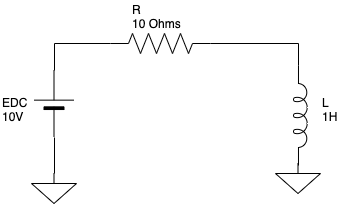
\includegraphics[width=0.7\textwidth]{img/thesissim1.png}
   \caption{DC Circuit}
   \label{thesissim1}
\end{figure}

\begin{lstlisting}[language=bash, label=getinfo, caption={Input data file for components in the Haskell implementation}, captionpos=b, label={lst:csv1r}]
Element Type,Node K,Node M,Value,Source param 1,Source param 2,Plot
EDC,2,0,10,0,0,0 
R,2,1,10,0,0,0
L,1,0,1,0,0,0
\end{lstlisting}


\begin{lstlisting}[language=bash, label=getinfo, caption={Input data file for time}, captionpos=b, label={lst:csv2r}]
Number of Nodes,Number of Voltages Sources,Step Size,Maximum time for simulation
2,1,0.0001,0.0005
\end{lstlisting}

The same setup in ETR-P is given by the file shown at \cref{lst:inputthtar}.

\begin{lstlisting}[language=bash, label=getinfo, caption={Original input data file for ETR-P Matlab}, captionpos=b, label={lst:inputthtar}]
T   2   1   100E-6  5E-4    0   0   0   0   0
EDC 2   0   10      0       0   0   0   0   5
R   2   1   10      0       0   0   0   0   5
L   1   0   1       0       0   0   0   0   5
NV  1   2   0       0       0   0   0   0   0
\end{lstlisting}


\subsection{ Short simulation with DC Voltage}

The simulation time is only 0.0005 seconds, which gives us only 6 \lstinline!npoints! for the step size of 0.0001. In a later section of this chapter, a longer simulation will be tested and executed.

In the Matlab version, it is possible to log the results from each iteration step by removing the semi-colons at the end of each line, or by explicitly calling the command \lstinline!fprintf!, as the example in \cref{lst:logthtar}.

\begin{lstlisting}[language=Matlab, label=getinfo, caption={Logging the results of V and I at the end of each iteration in Matlab}, captionpos=b, label={lst:logthtar}]
%% Build vector IA for the time t
    IA = I(1:D, 1);
    
    %% Build the vector RHSA for the time t
    RHSA = IA - GAB*VB;
    
    %% Solve for vector VA at the time t
    VA = GAA\RHSA;
    IB = GBA*VA+GBB*VB;
    I = [IA; IB];
    %% Build vector V at the time t (i.e.,  time counter or point n)
    V(:, n) = [VA; VB];
    
    fprintf('---------------- I final in every step of the loop -----------\n');
    I
    fprintf('---------------- V final in every step of the loop -----------\n');
    V
\end{lstlisting}

Logging and debugging is not equally straightforward in Haskell. A log would represent an impurity, since it writes at the standard output. To print out the values of operations in pure functions, it is necessary to use the \lstinline!Debug.Trace! library. To log the values of \lstinline!I! and \lstinline!V! in every iteration, there must be a call to the \lstinline!Trace.trace! function in some of the let binding in the \lstinline!thtaSimulationStep! function. Example in \cref{lst:logginghs}.

\begin{lstlisting}[language=Haskell, numbers=left, caption={Logging the values of I and V at the Haskell implementation}, captionpos=b, label={lst:logginghs}]
thtaSimulationStep :: [ComponentData] -> Matrix Double -> [Double] -> SimulationData -> Int -> Int -> Double  -> Vector Double -> Matrix Double -> Vector Double -> Vector Double -> SimulationResults
thtaSimulationStep _ _ _ _ _ 1 _ _ vMatrix _ iVector = (iVector, vMatrix)
thtaSimulationStep components condutances gkms simulation thtactl n time ih vMatrix vbVector iVector =
  let (gaa, gab, gba, gbb) = Matrix.splitBlocks ((nodes simulation) - (voltageSources simulation)) ((nodes simulation) - (voltageSources simulation)) condutances
      ihBuffer = buildIhVector components gkms n ih (Vector.replicate (nh (Vector.fromList components)) 0) vMatrix
      vbVec = buildVBVector components
      (thta, ihThta, timeThta) = thtaControl thtactl time ihBuffer ih
      iVec = buildIVector components ihThta (Vector.replicate (nodes simulation) 0)
      (iVecCalc, vVec) = Trace.trace ("Solver = \n" ++ show (solver (toHMatrixVectorTransformer iVec) (toHMatrixTransformer gaa) (toHMatrixTransformer gab) (toHMatrixTransformer gba) (toHMatrixTransformer gbb) (toHMatrixVectorTransformer vbVec) simulation)) solver (toHMatrixVectorTransformer iVec) (toHMatrixTransformer gaa) (toHMatrixTransformer gab) (toHMatrixTransformer gba) (toHMatrixTransformer gbb) (toHMatrixVectorTransformer vbVec) simulation
      vMatr = Trace.trace ("vMatrix = \n" ++ show (Matrix.mapCol (\r _ -> vVec Vector.! (r - 1)) (n-1) vMatrix)) Matrix.mapCol (\r _ -> vVec Vector.! (r - 1)) (n-1) vMatrix
  in
      thtaSimulationStep components condutances gkms simulation thta (n-1) time ihThta vMatr vbVec iVecCalc

\end{lstlisting}

\subsubsection{Step 0}
Initial step. Everything is set to 0.0.

\subsubsection{Step 1}

Results in Haskell - \cref{h1}:

\begin{figure}[H]
   \centering
   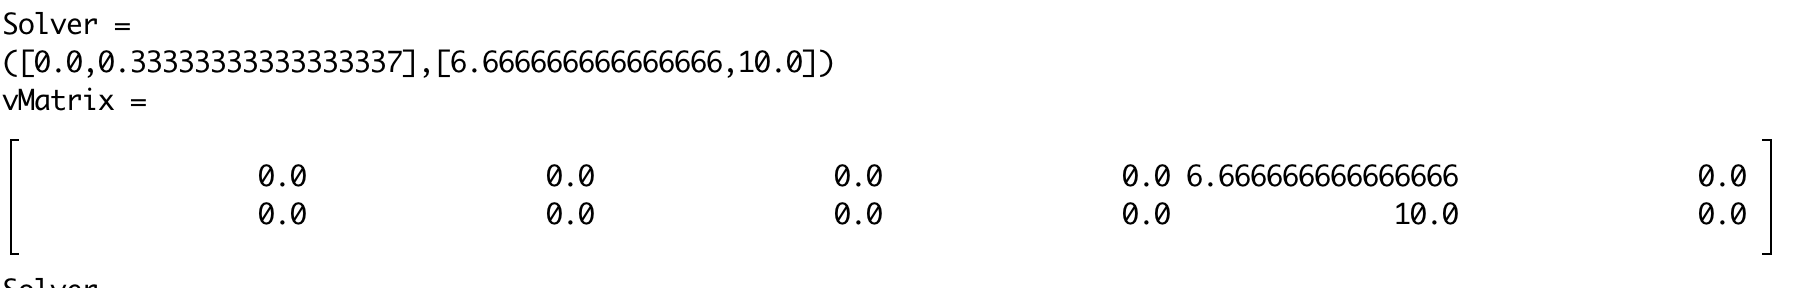
\includegraphics[width=0.9\textwidth]{img/h1.png}
   \caption{Results for step 5 - Haskell (recall that the Haskell loop stars from the highest value of the iteration, which is 5)}
   \label{h1}
\end{figure}

Results form Matlab - \cref{m1}:

\begin{figure}[H]
   \centering
   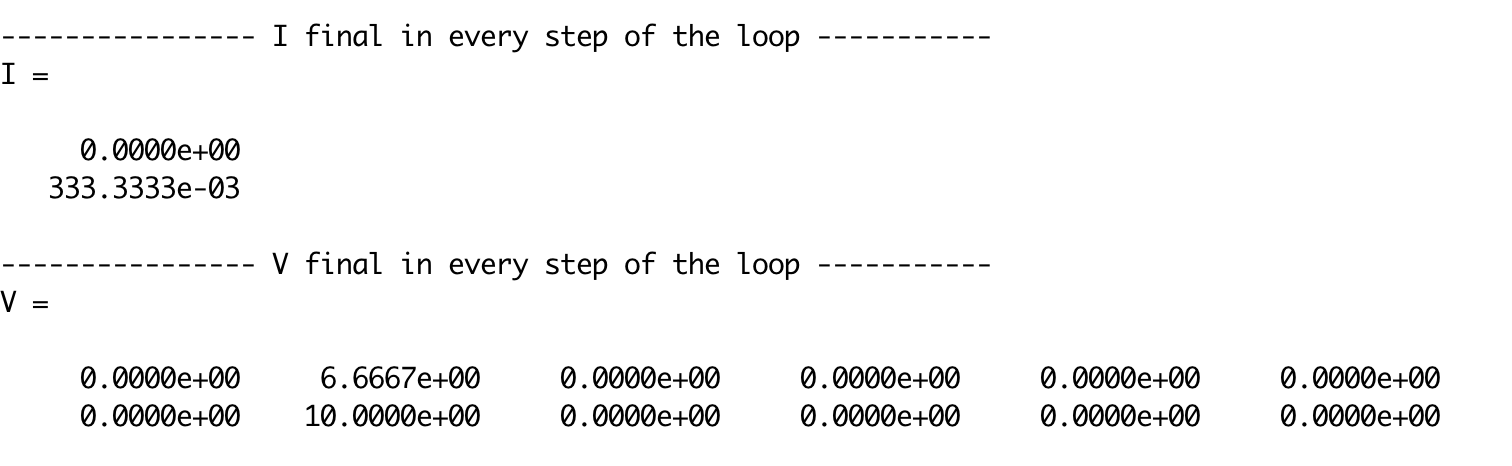
\includegraphics[width=0.9\textwidth]{img/m1.png}
   \caption{Results for step 1 - Matlab}
   \label{m1}
\end{figure}


\subsubsection{Step 2}

Results in Haskell - \cref{h2}:

\begin{figure}[H]
   \centering
   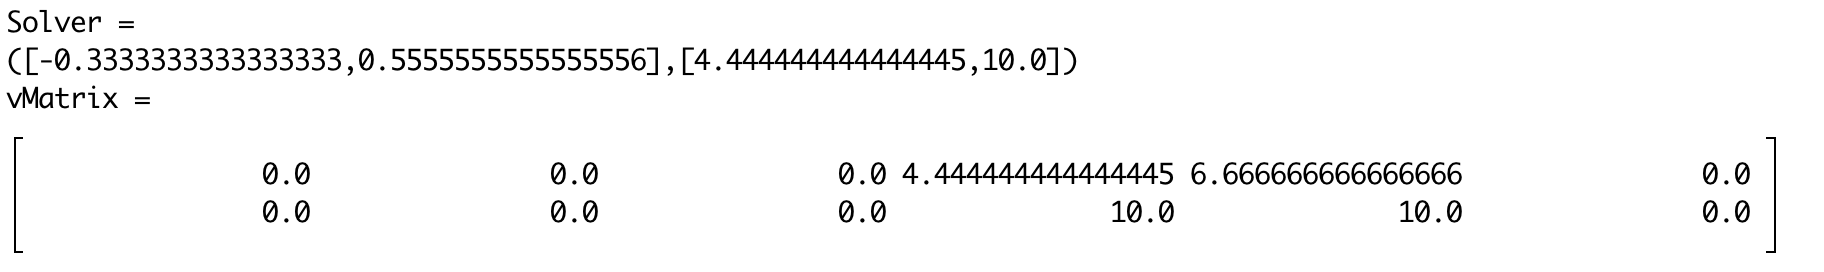
\includegraphics[width=0.9\textwidth]{img/h2.png}
   \caption{Results for step 4 - Haskell}
   \label{h2}
\end{figure}

Results form Matlab - \cref{m2}:

\begin{figure}[H]
   \centering
   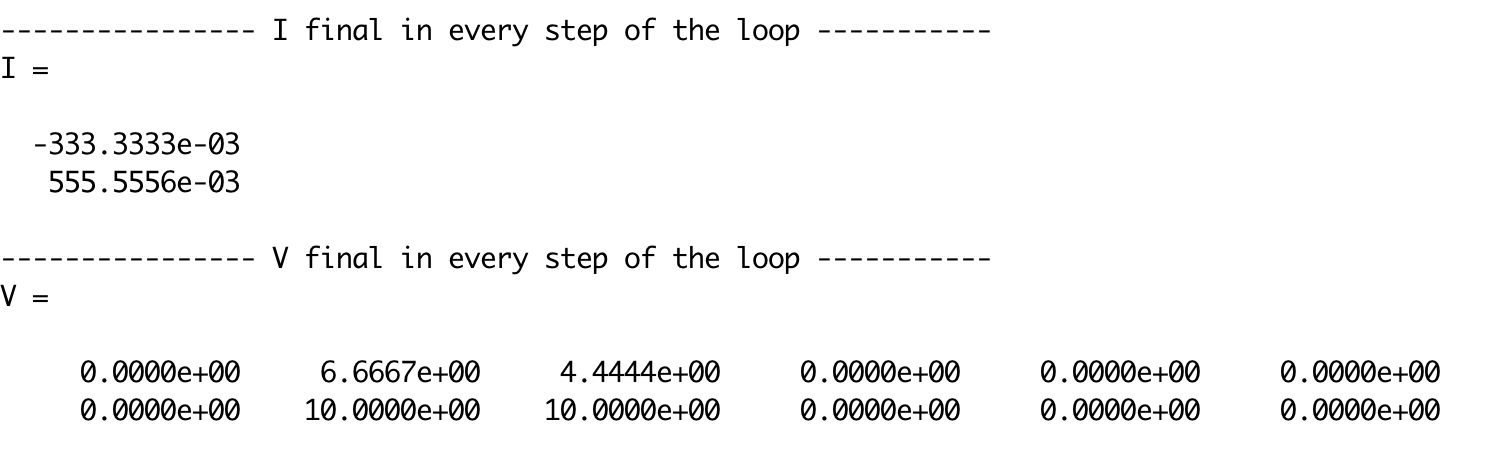
\includegraphics[width=0.9\textwidth]{img/m2.png}
   \caption{Results for step 2 - Matlab}
   \label{m2}
\end{figure}


\subsubsection{Step 3}

Results in Haskell - \cref{h3}:

\begin{figure}[H]
   \centering
   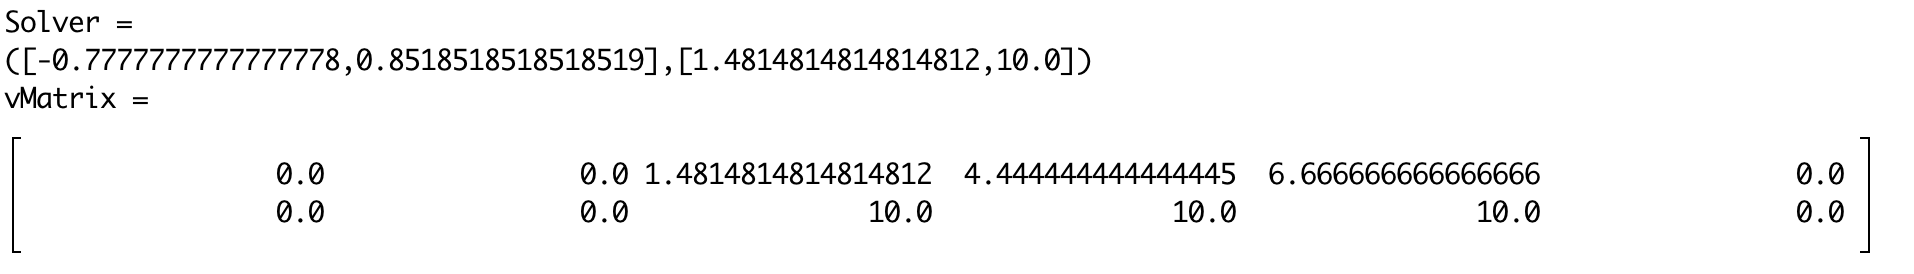
\includegraphics[width=0.9\textwidth]{img/h3.png}
   \caption{Results for step 3 - Haskell}
   \label{h3}
\end{figure}

Results form Matlab - \cref{m3}:

\begin{figure}[H]
   \centering
   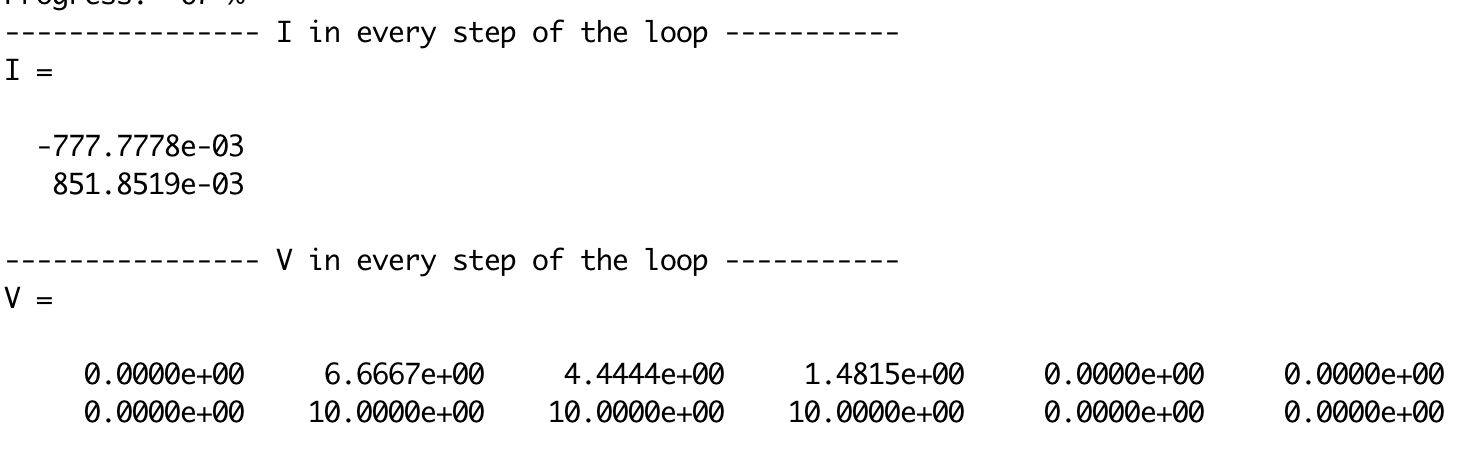
\includegraphics[width=0.9\textwidth]{img/m3.png}
   \caption{Results for step 3 - Matlab}
   \label{m3}
\end{figure}


\subsubsection{Step 4}

Results in Haskell - \cref{h5}:

\begin{figure}[H]
   \centering
   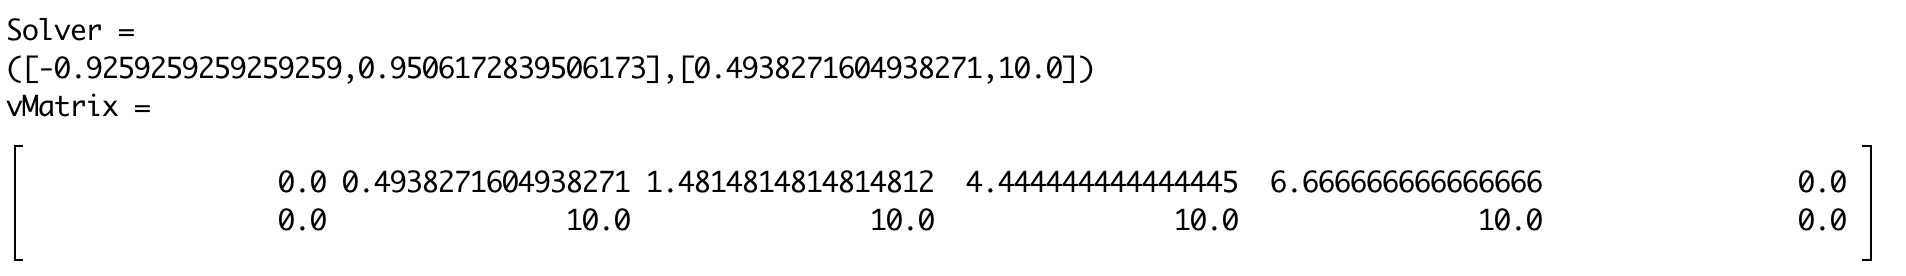
\includegraphics[width=0.9\textwidth]{img/h5.png}
   \caption{Results for step 2 - Haskell}
   \label{h5}
\end{figure}

Results form Matlab - \cref{m5}:

\begin{figure}[H]
   \centering
   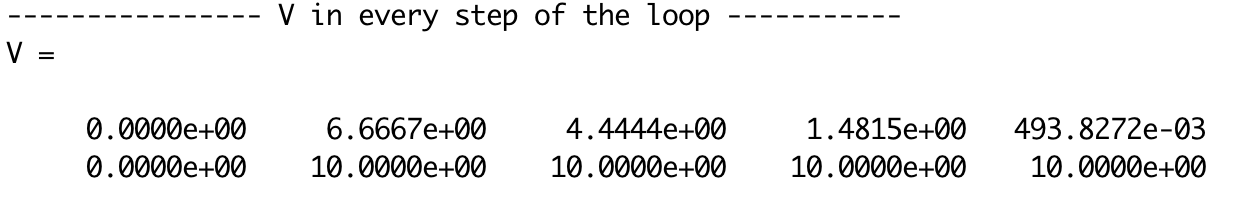
\includegraphics[width=0.7\textwidth]{img/m5.png}
   \caption{Results for step 4 - Matlab}
   \label{m5}
\end{figure}


\subsubsection{Step 5 - final step}


Figure \ref{reschart1} is a plot of both simulations for the voltage outputs of the V Matrix. There are no significant differences between the results and the curves are on the same place.


\begin{figure}[H]
   \centering
   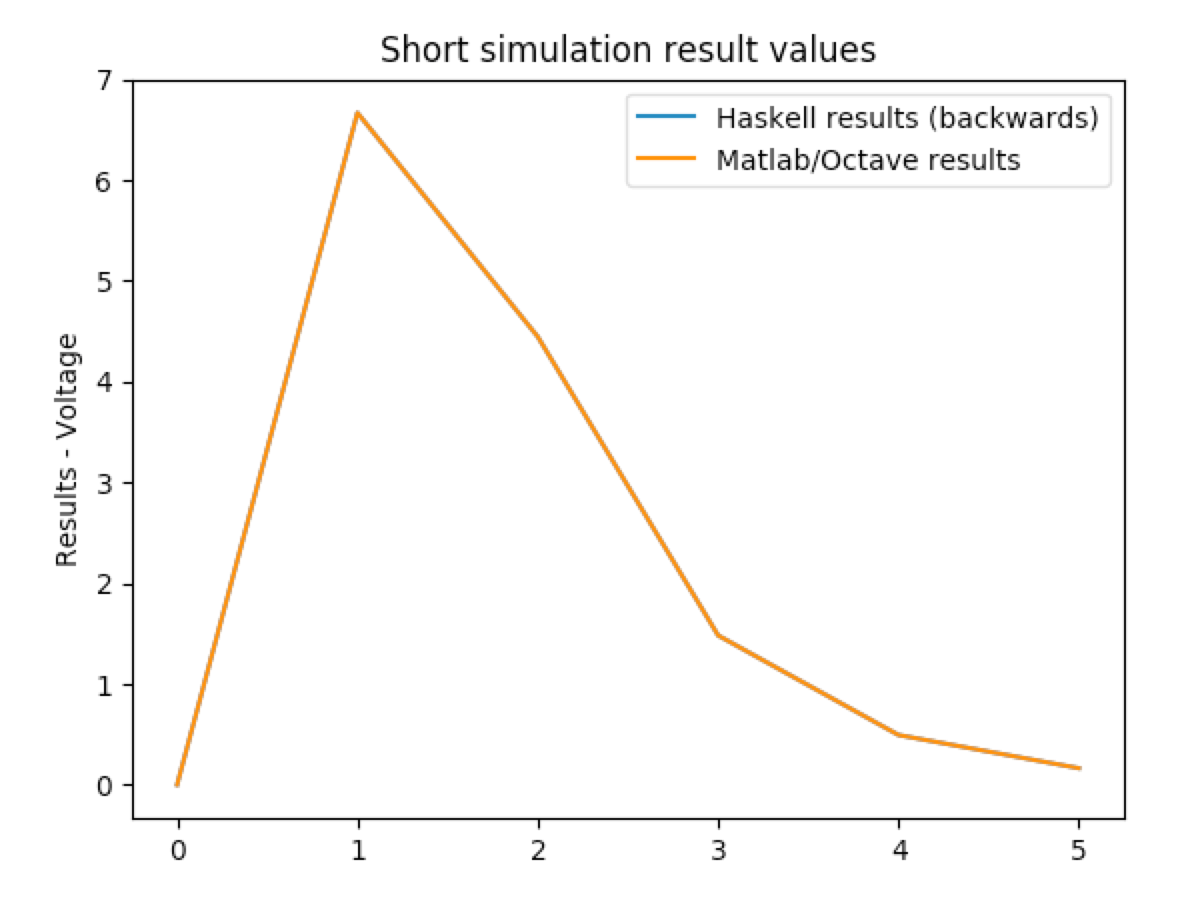
\includegraphics[width=0.7\textwidth]{img/voltageplot.png}
   \caption{Short simulation results chart - V}
   \label{reschart1}
\end{figure}

Figure \ref{iachart} and \cref{ibchart} are the chars for IA and IB results, respectively:

\begin{figure}[H]
   \centering
   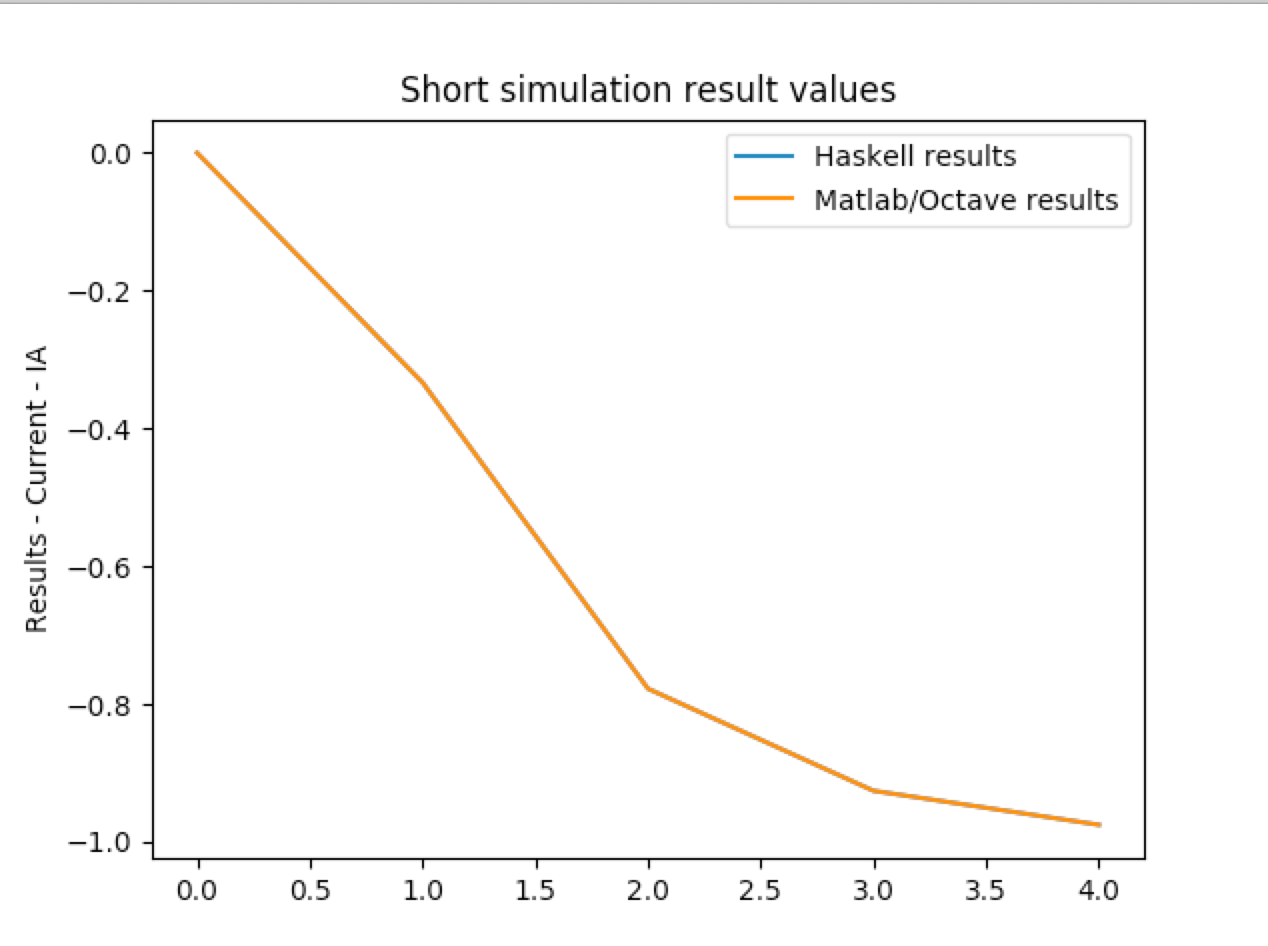
\includegraphics[width=0.7\textwidth]{img/iaplot.png}
   \caption{Short simulation results chart - IA}
   \label{iachart}
\end{figure}



\begin{figure}[H]
   \centering
   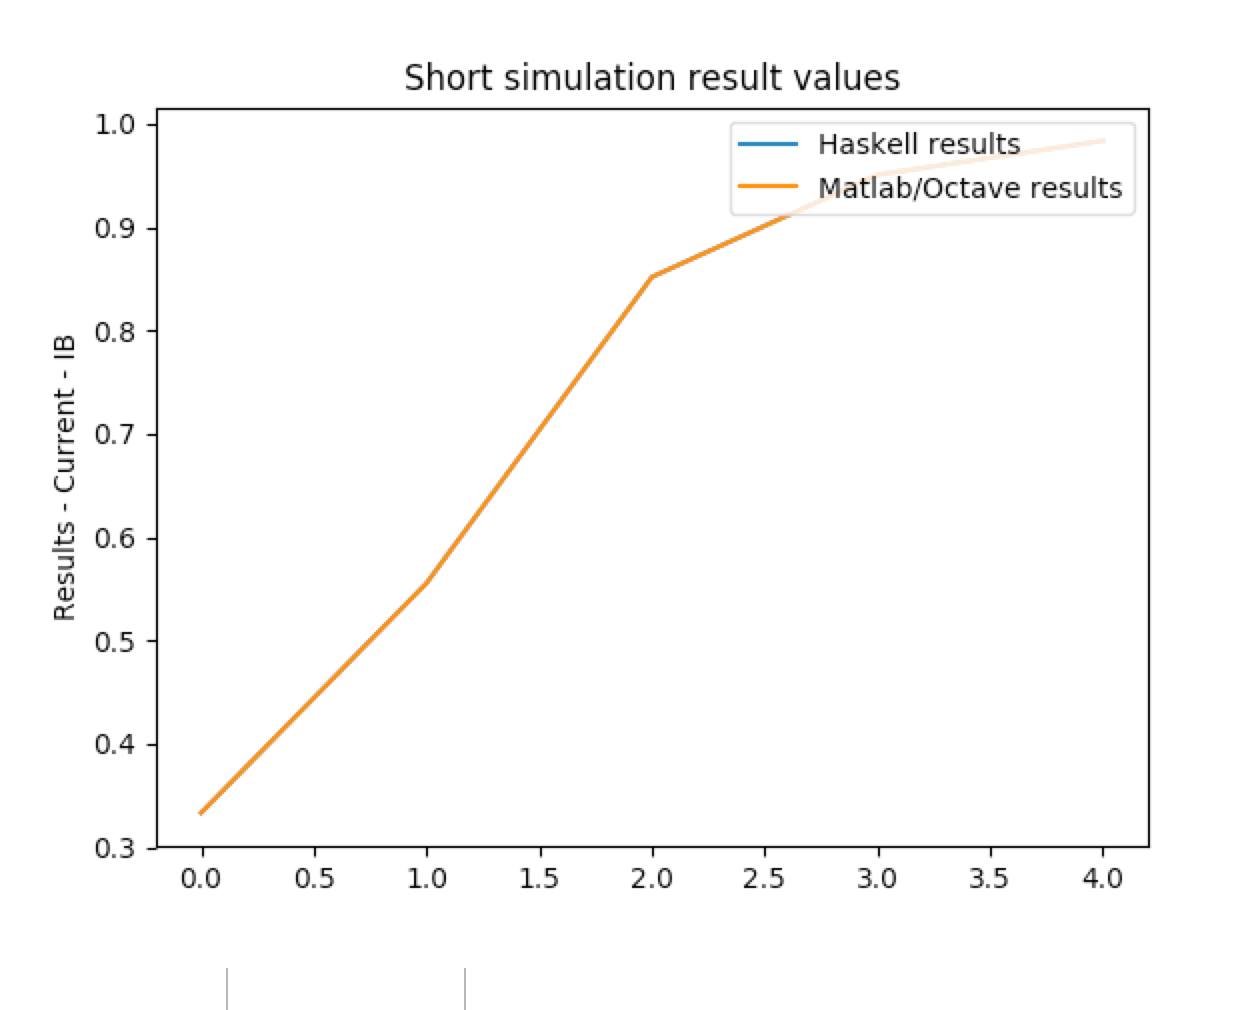
\includegraphics[width=0.9\textwidth]{img/ibplot.png}
   \caption{Short simulation results chart - IB}
   \label{ibchart}
\end{figure}

Note: The charts were plotted using Python to avoid bias towards the two languages during the comparison process.

The final V Matrix is described in \cref{tab:hsresults}.

% Please add the following required packages to your document preamble:
% \usepackage{graphicx}
\begin{table}[H]
\resizebox{\textwidth}{!}{%
\begin{tabular}{llllll}
Step 5              & Step 4             & Step 3             & Step 2            & Step 1            & Step 0 \\
0.16460905349794236 & 0.4938271604938271 & 1.4814814814814812 & 4.444444444444445 & 6.666666666666666 & 0.0    \\
10.0                & 10.0               & 10.0               & 10.0              & 10.0              & 0.0   
\end{tabular}%
}
\caption{V Matrix calculated for the Haskell implementation. The results go from right to left. Each column represents one step of the iteration}
\label{tab:hsresults}
\end{table}

The final V Matrix from the Matlab implementation is listed in \cref{tab:thtamatlabv}.

% Please add the following required packages to your document preamble:
% \usepackage{graphicx}
\begin{table}[H]
\resizebox{\textwidth}{!}{%
\begin{tabular}{llllll}
Step 0     & Step 1      & Step 2      & Step 3      & Step 4       & Step 5      \\
0.0000e+00 & 6.6667e+00  & 4.4444e+00  & 1.4815e+00  & 493.8272e-03 & 164.6091e-03 \\
0.0000e+00 & 10.0000e+00 & 10.0000e+00 & 10.0000e+00 & 10.0000e+00  & 10.0000e+00
\end{tabular}%
}
\caption{V Matrix calculated for the Matlab implementation. The results go from left to right.}
\label{tab:thtamatlabv}
\end{table}

It is important to also compare the results from the \lstinline!I! Vector. For the Haskell implementation, the final values are $ [-0.9753086419753086,0.9835390946502057] $ and for the Matlab ETR-P, the values are $ [-975.3086e-03, 983.5391e-03] $. As expected, those are very close values (numerically).


\subsection{ Long simulation with DC Voltage }
\label{longsimmm}

With some initial guarantees of a successful short simulation, it becomes reasonable to run a longer simulation (setting up \lstinline!tmax! for 0.05) and then compare the results. 

When analysing the final \lstinline!V! Matrices of this longer simulation, it is possible to notice they will be both square and triangular matrices. Several values will be either 0.0 or 10.0 (EDC Voltage source). The transient, calculated values are compared in \ref{fig:haskellvmatrfinal}.

\begin{figure}[H]
   \centering
   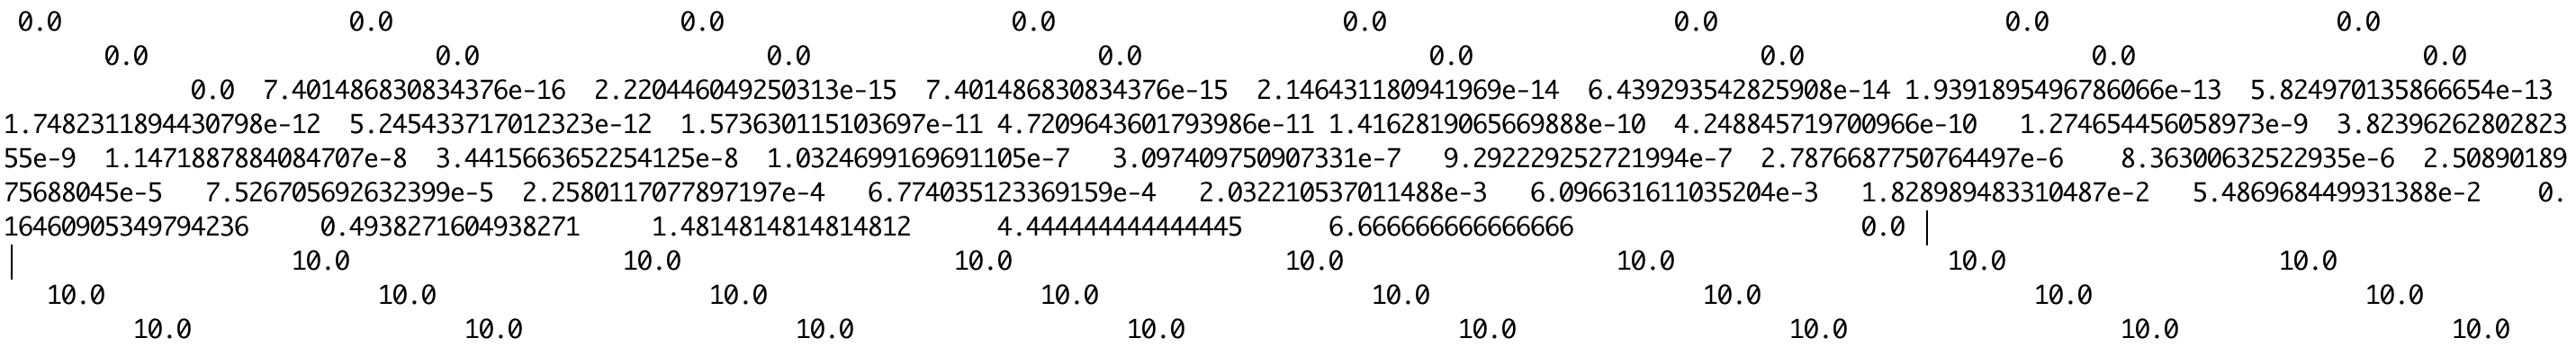
\includegraphics[width=0.9\textwidth]{img/results_Haskell.png}
   \caption{Results for the triangular Matrix V in a broader simulation with Haskell}
   \label{fig:haskellvmatrfinal}
\end{figure}


\begin{figure}[H]
   \centering
   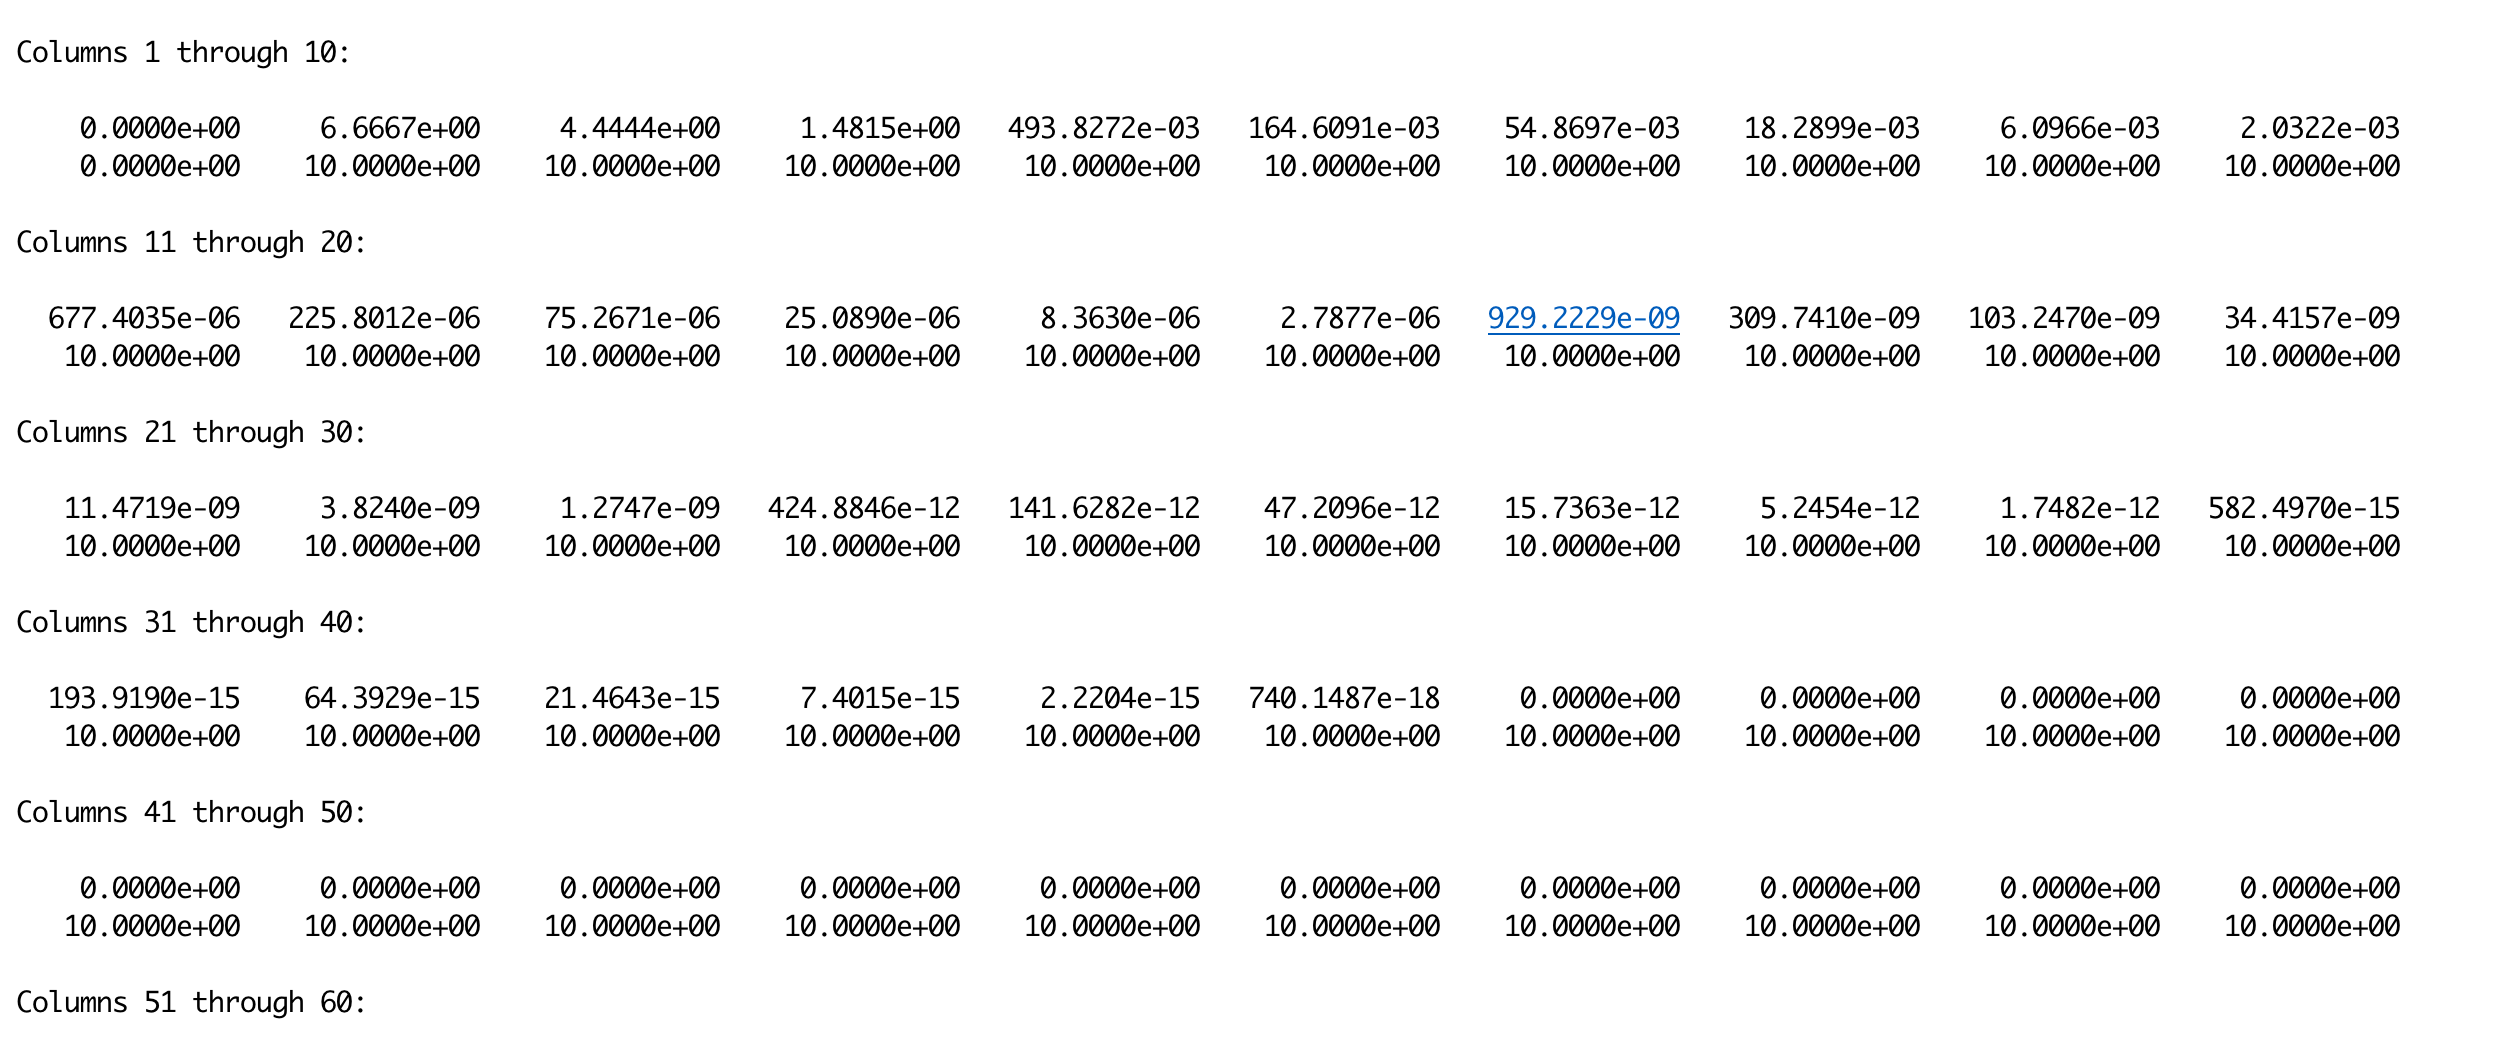
\includegraphics[width=0.9\textwidth]{img/results_THTA_Matlab.png}
   \caption{Results for the triangular Matrix V in a broader simulation with THTA Matlab}
   \label{matlabvmatrfinal}
\end{figure}

Compare the first value of the figure \ref{fig:haskellvmatrfinal} (7.401486830834376e-16) with the last result which is not 0 at \ref{matlabvmatrfinal}. By contrasting first and last pairs, it is possible to notice the values are very similar (numerically). It is then demonstrated that the program works as expected according to the ETR-P algorithm.


Figure \ref{reschart2} is a plot of both simulations for the voltage outputs of the V Matrix in this longer simulation. There are no significant differences between the results. Only the transient values appear in this plot to allow the value comparison.


\begin{figure}[H]
   \centering
   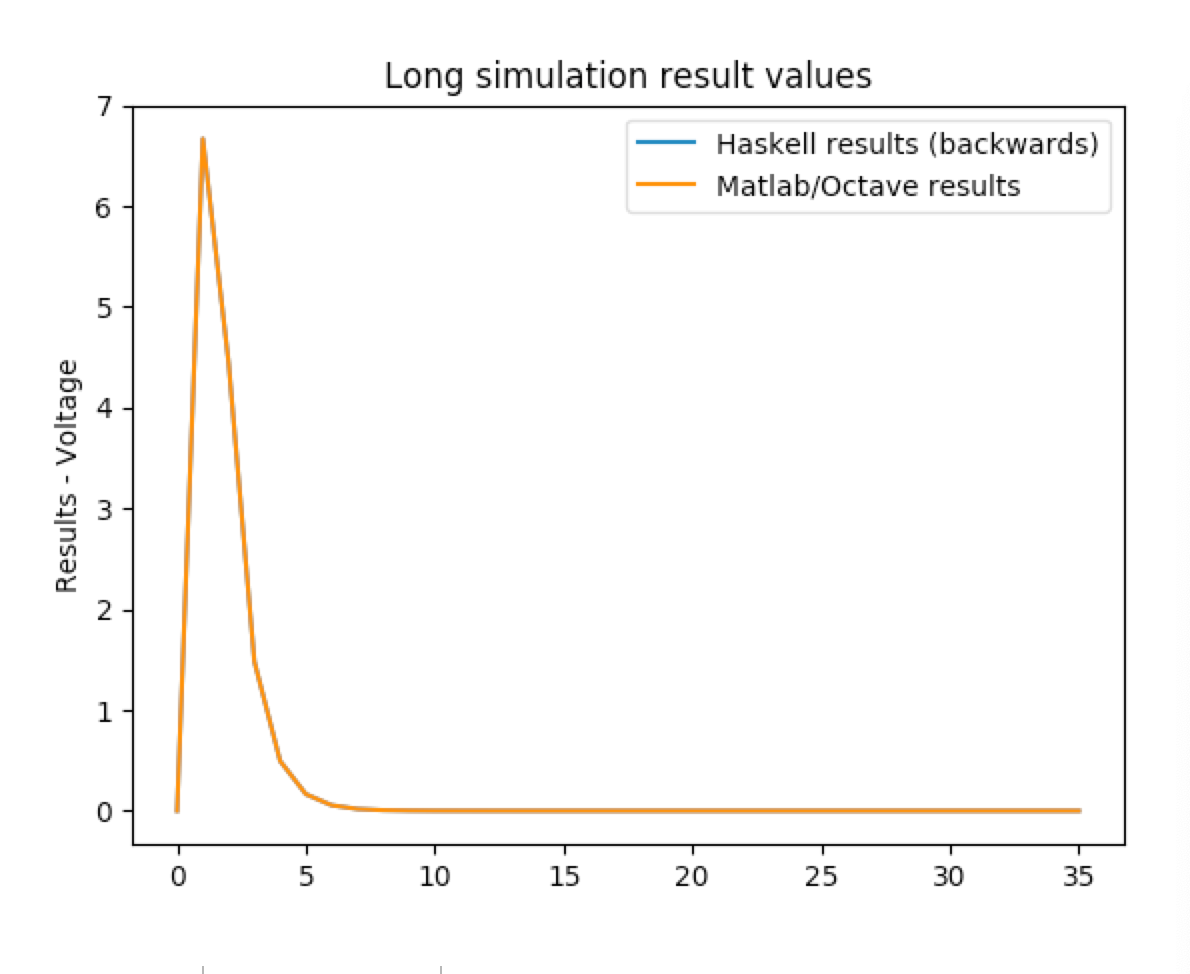
\includegraphics[width=0.7\textwidth]{img/voltageplotlong.png}
   \caption{Long simulation results chart - V}
   \label{reschart2}
\end{figure}

Note: The chart was plotted using Python to avoid bias towards the two languages during the comparison process.

Once again the results are pretty accurate and result in two overlapping curves.

Next, \cref{fig:dcresultsmicro} and \cref{fig:dcresultsmicrooctave} shows the results for the voltage outputs when setting up \lstinline!tmax! for 0.01s and the step size of 0.000001s.

\begin{figure}[H]
   \centering
   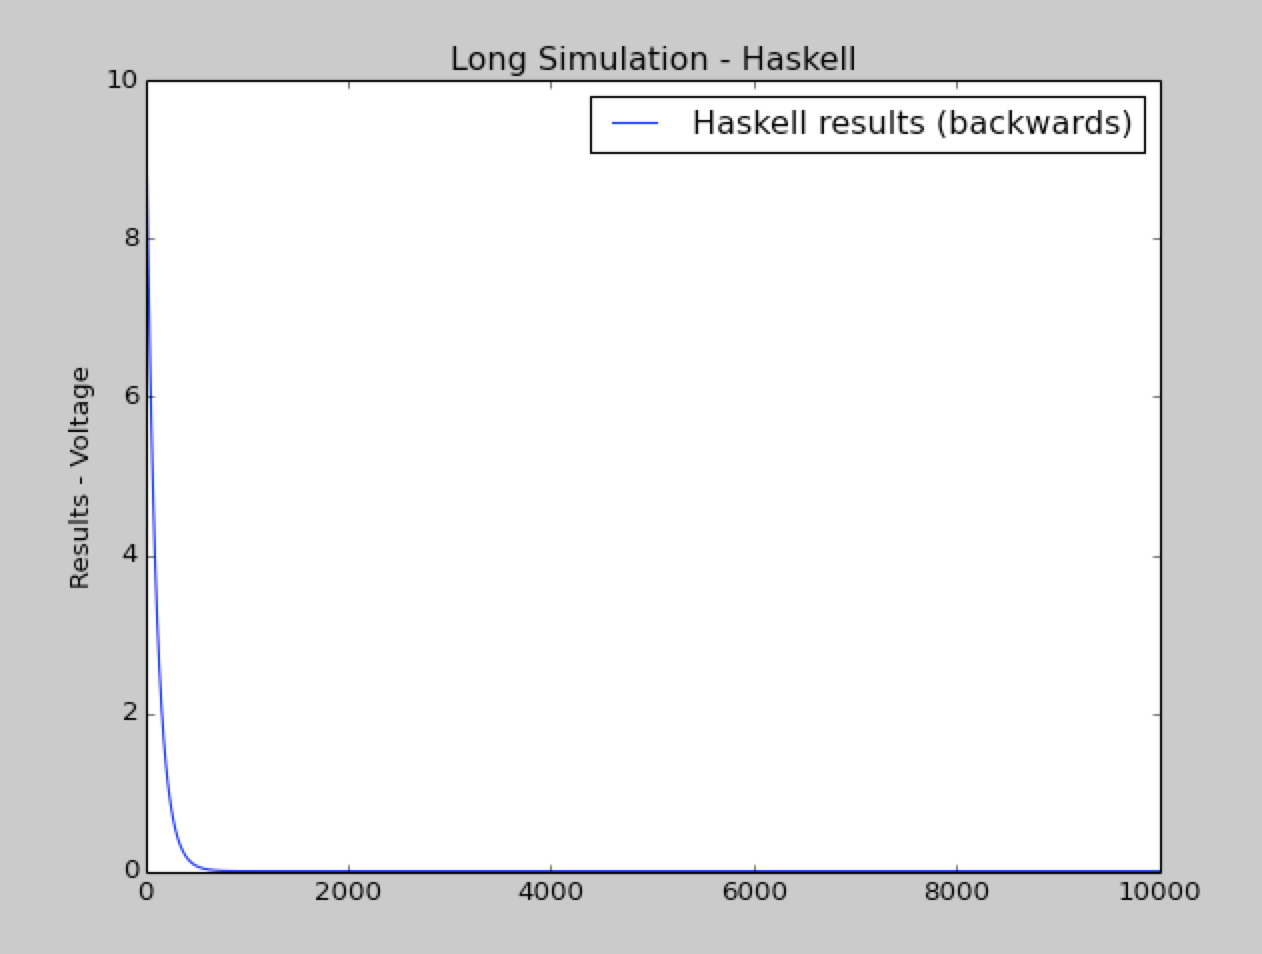
\includegraphics[width=0.7\textwidth]{img/dcresultsmicro.png}
   \caption{DC Circuit, Haskell implementation, step size of 0.000001s}
   \label{fig:dcresultsmicro}
\end{figure}

\begin{figure}[H]
   \centering
   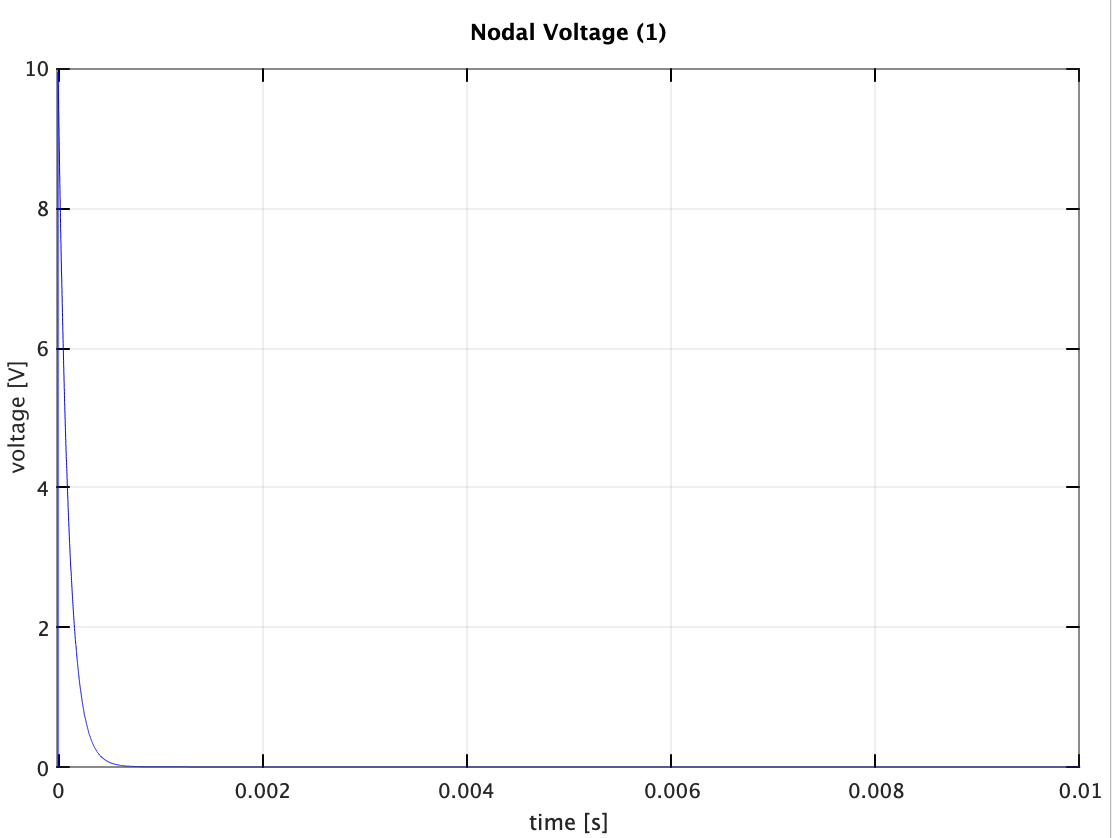
\includegraphics[width=0.7\textwidth]{img/dcresultsmicrooctave.png}
   \caption{DC Circuit, Matlab implementation, step size of 0.000001s}
   \label{fig:dcresultsmicrooctave}
\end{figure}


\subsection{Short simulation with AC Voltage}

The results for the short AC simulation (with an EAC source component) are similar for both the implementations. Listing \ref{lst:inputthtareac} is the configuration for the Matlab version, and \cref{lst:csv1reac} for the Haskell version. The circuit is described in \cref{eacresults2}.

\begin{figure}[H]
   \centering
   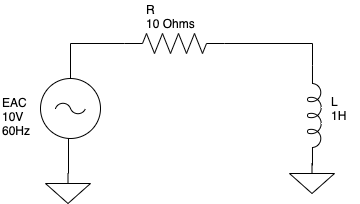
\includegraphics[width=0.7\textwidth]{img/eacresults2.png}
   \caption{AC Circuit}
   \label{eacresults2}
\end{figure}


\begin{lstlisting}[language=bash, caption={Original input data file for ETR-P Matlab}, captionpos=b, label={lst:inputthtareac}]
T   2   1   100E-6  5E-4   0   0   0   0   0
EAC 2   0   10       0      60  0   0   0   5
R   2   1   10       0      0   0   0   0   5
L   1   0   1        0      0   0   0   0   5
NV  1   2   0        0      0   0   0   0   0
\end{lstlisting}

\begin{lstlisting}[language=bash, label=getinfo, caption={Input data file for components in the Haskell implementation}, captionpos=b, label={lst:csv1reac}]
Element Type,Node K,Node M,Value,Source param 1,Source param 2,Plot
EAC,2,0,10,0,60,0
R,2,1,10,0,0,0
L,1,0,1,0,0,0
\end{lstlisting}

The results for the \lstinline!I! Vector with this configuration in Matlab are \lstinline![-970.3633e-03, 976.4595e-03]! and \lstinline![-0.9703633353209364,0.9764594717932623]! for the Haskell implementation. \ref{eacmatlab} and \ref{eachaskell} bring a comparison for the Voltage matrices in both implementations. 


\begin{figure}[H]
   \centering
   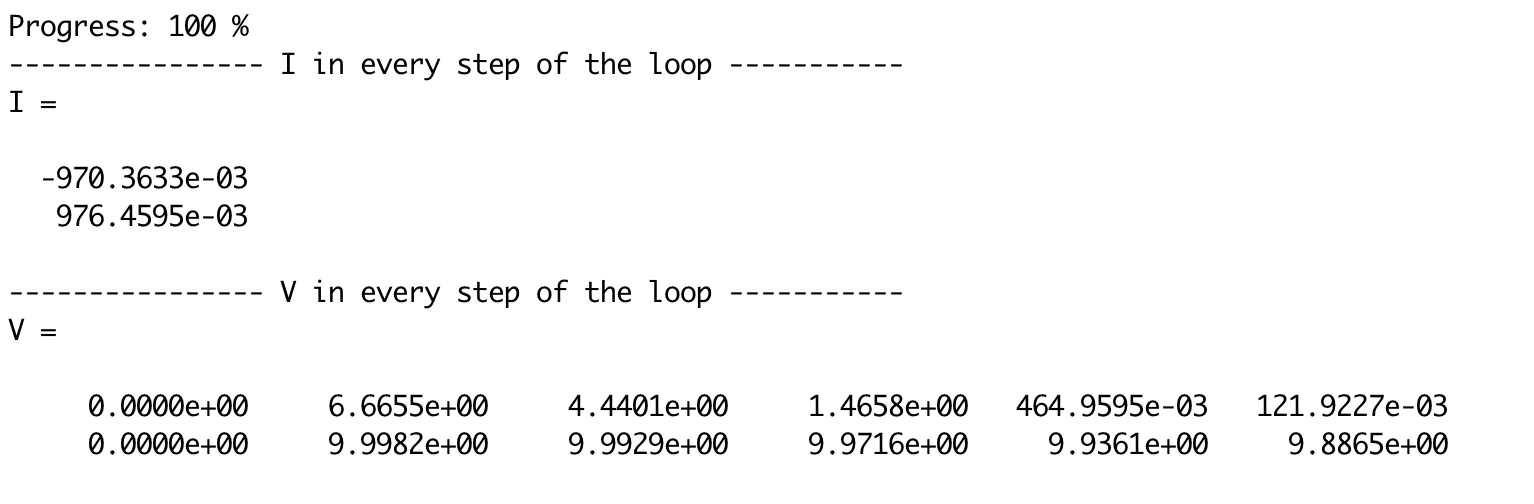
\includegraphics[width=0.7\textwidth]{img/eacmatlab.png}
   \caption{Matlab implementation - AC Voltage Source}
   \label{eacmatlab}
\end{figure}

\begin{figure}[H]
   \centering
   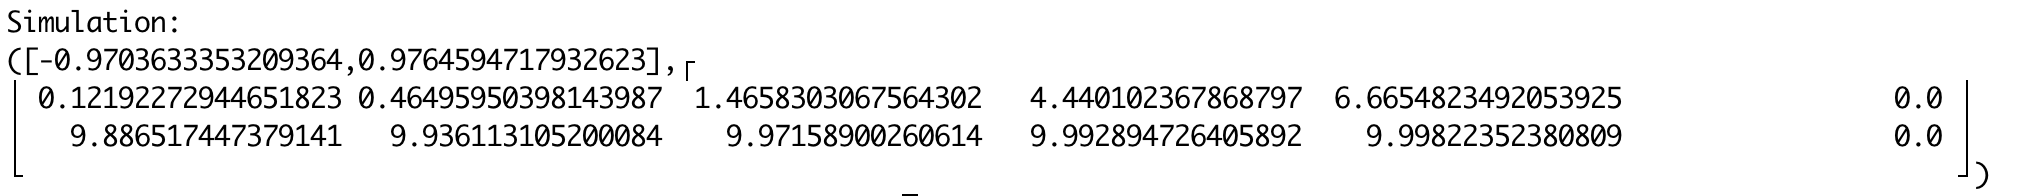
\includegraphics[width=0.7\textwidth]{img/eachaskell.png}
   \caption{Haskell implementation - AC Voltage Source}
   \label{eachaskell}
\end{figure}


\section{Simulation outputs - RC Circuit}

\subsection{Short simulation with DC Voltage}

Running a short simulation for a RC Circuit with the setup specified on \cref{lst:csv1capacitor} and \cref{lst:csv1capacitorsimulation}, it is possible to obtain the results listed on \cref{capacitorcomparison}. Once again the voltage values for the node 1 are the same in both Matlab (see \cref{capacitorcomparisonmatlab}) and Haskell (see \cref{capacitorcomparisonhaskell}) implementations. 

\begin{lstlisting}[language=bash, label=getinfo, caption={Input data file for components in the Haskell implementation}, captionpos=b, label={lst:csv1capacitor}]
Element Type,Node K,Node M,Value,Source param 1,Source param 2,Plot
EDC,2,0,10,0,60,0
R,2,1,10,0,0,0
C,1,0,1,0,0,0
\end{lstlisting}


\begin{lstlisting}[language=bash, label=getinfo, caption={Input data file for components in the Haskell implementation}, captionpos=b, label={lst:csv1capacitorsimulation}]
Number of Nodes,Number of Voltages Sources,Step Size,Maximum time for simulation
2,1,0.0001,0.0005
\end{lstlisting}

\begin{figure}[H]
   \centering
   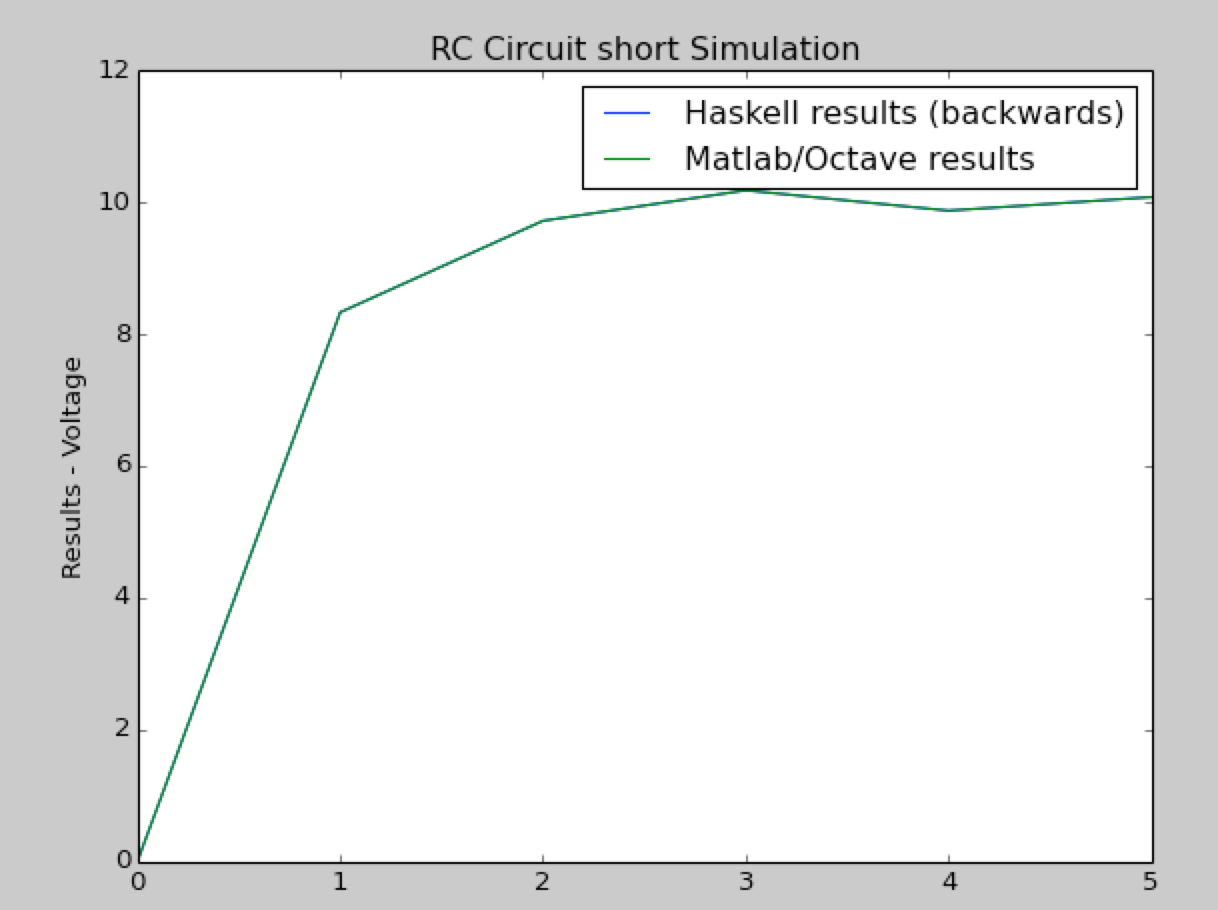
\includegraphics[width=0.7\textwidth]{img/capacitorcomparison.png}
   \caption{Comparison - DC Voltage Source for a RC Circuit}
   \label{capacitorcomparison}
\end{figure}

\begin{figure}[H]
   \centering
   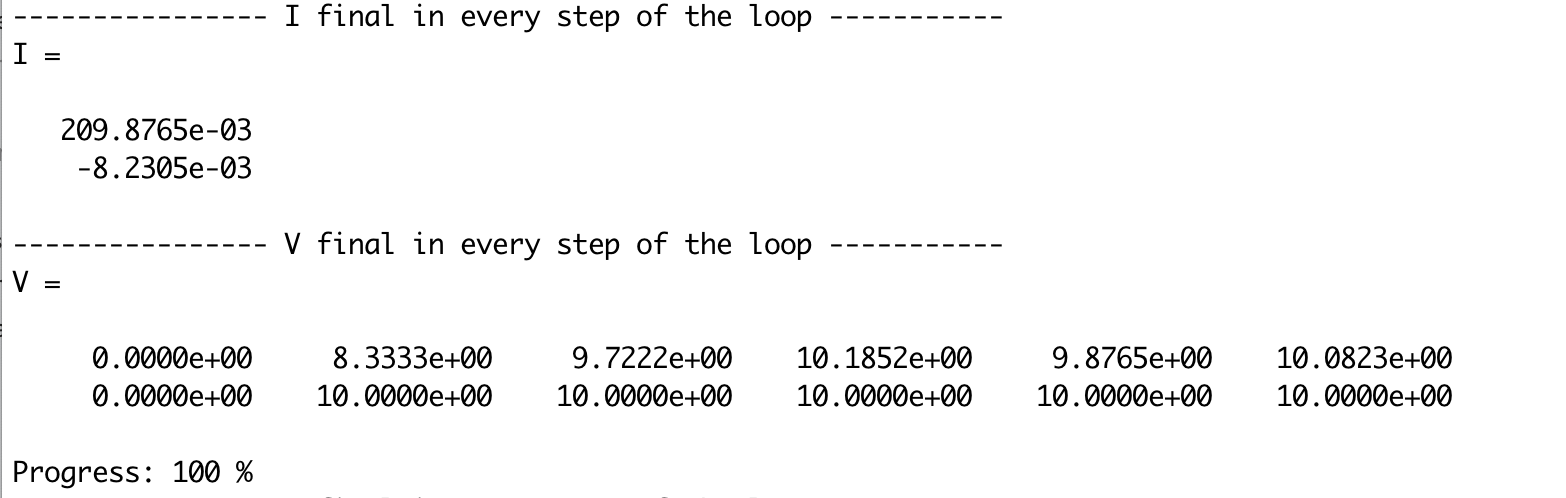
\includegraphics[width=0.7\textwidth]{img/capacitorcomparisonmatlab.png}
   \caption{Matlab results - DC Voltage Source for a RC Circuit}
   \label{capacitorcomparisonmatlab}
\end{figure}

\begin{figure}[H]
   \centering
   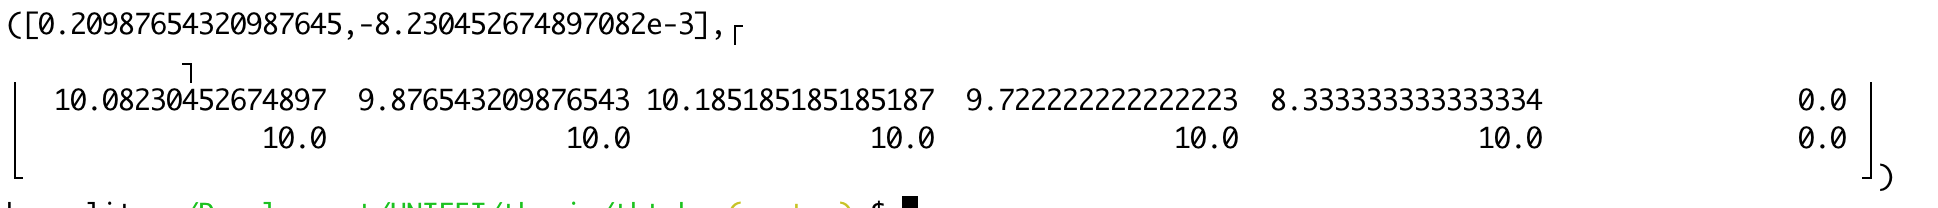
\includegraphics[width=0.7\textwidth]{img/capacitorcomparisonhaskell.png}
   \caption{Haskell results - DC Voltage Source for a RC Circuit}
   \label{capacitorcomparisonhaskell}
\end{figure}


\subsection{Short simulation with AC Voltage}

Running a short simulation for a RC Circuit with an AC source according to the setup specified on \cref{lst:csv2capacitor} and \cref{lst:csv2capacitorsimulation}, it is possible to obtain the results listed on \cref{capacitorcomparison2}. Once again the voltage values for the node 1 are the same in both Matlab (see \cref{capacitorcomparisonmatlab2}) and Haskell (see \cref{capacitorcomparisonhaskell2}) implementations. 

\begin{lstlisting}[language=bash, label=getinfo, caption={Input data file for components in the Haskell implementation}, captionpos=b, label={lst:csv2capacitor}]
Element Type,Node K,Node M,Value,Source param 1,Source param 2,Plot
EAC,2,0,10,0,60,0
R,2,1,10,0,0,0
C,1,0,1,0,0,0
\end{lstlisting}


\begin{lstlisting}[language=bash, label=getinfo, caption={Input data file for components in the Haskell implementation}, captionpos=b, label={lst:csv2capacitorsimulation}]
Number of Nodes,Number of Voltages Sources,Step Size,Maximum time for simulation
2,1,0.0001,0.0005
\end{lstlisting}

\begin{figure}[H]
   \centering
   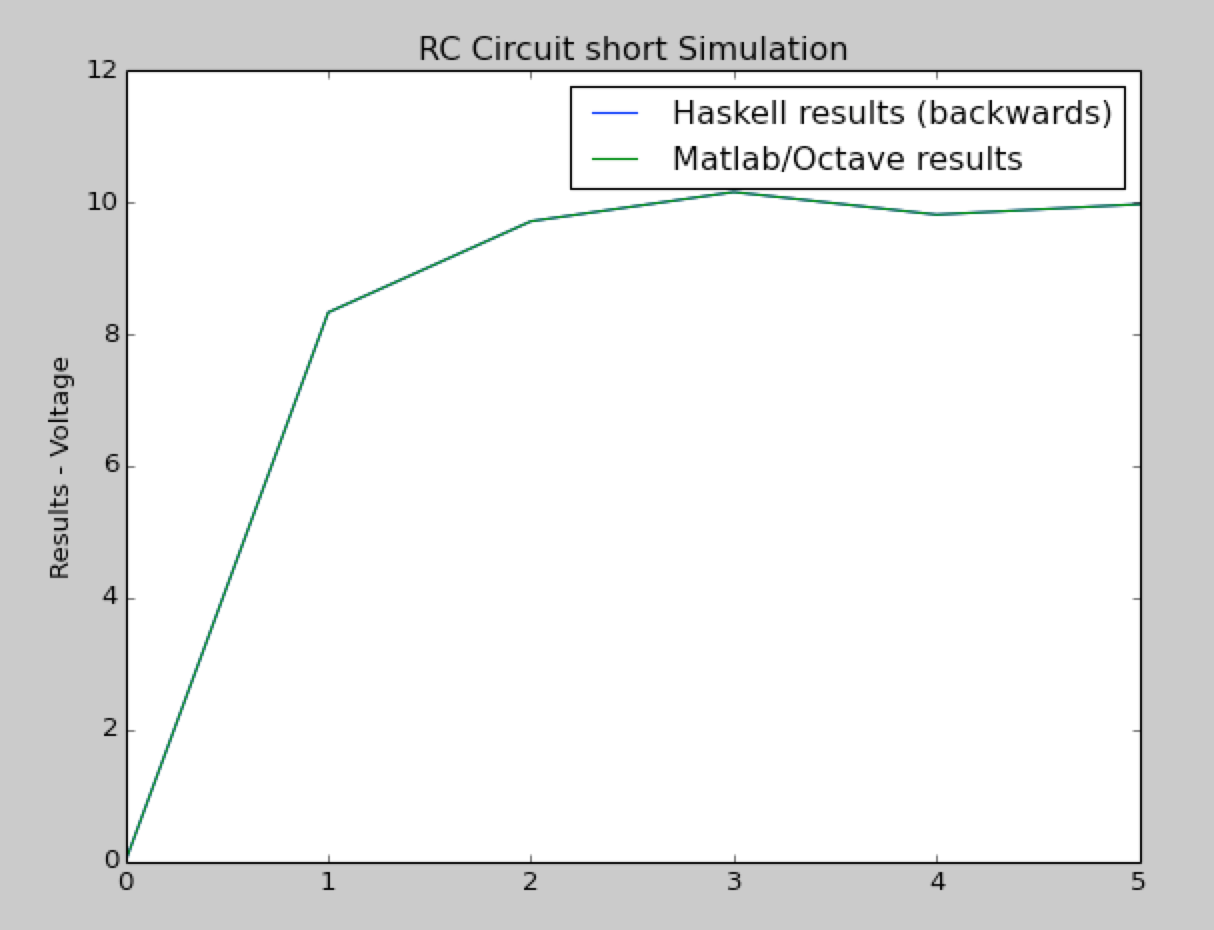
\includegraphics[width=0.7\textwidth]{img/capacitorcomparison2.png}
   \caption{Comparison - AC Voltage Source for a RC Circuit}
   \label{capacitorcomparison2}
\end{figure}

\begin{figure}[H]
   \centering
   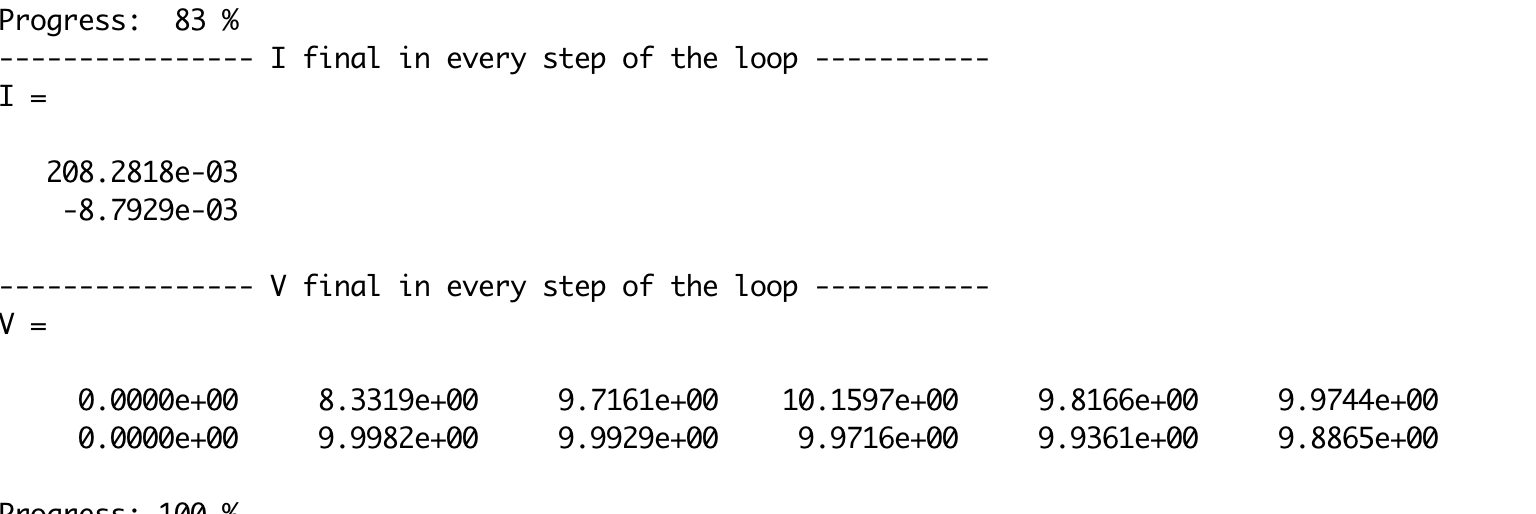
\includegraphics[width=0.7\textwidth]{img/capacitorcomparisonmatlab2.png}
   \caption{Matlab results - AC Voltage Source for a RC Circuit}
   \label{capacitorcomparisonmatlab2}
\end{figure}

\begin{figure}[H]
   \centering
   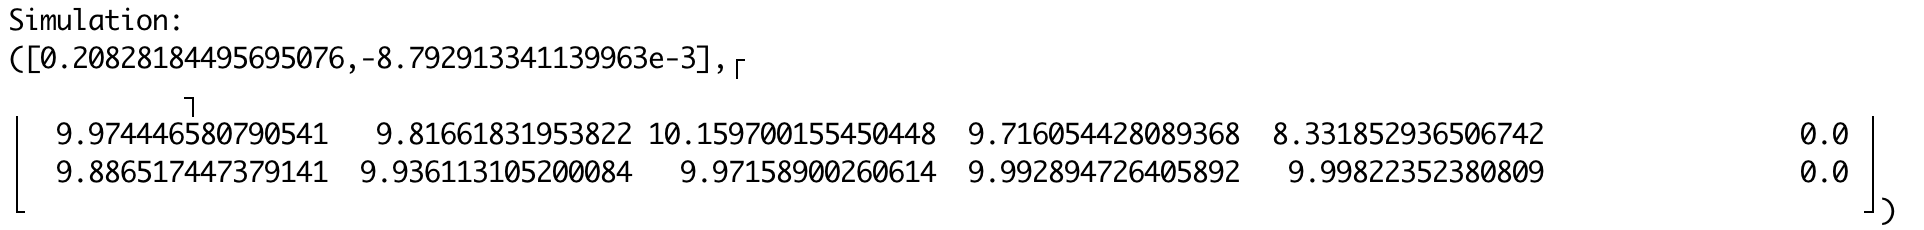
\includegraphics[width=0.7\textwidth]{img/capacitorcomparisonhaskell2.png}
   \caption{Haskell results - AC Voltage Source for a RC Circuit}
   \label{capacitorcomparisonhaskell2}
\end{figure}

\section{Recursion problems}

One of the downsides of the Haskell language was the performance of the recursive calls. Even though optimisation and execution time analysis are not the main focus of this work, it is important to mention that the overall execution time for the Haskell version of the ETR-P was slower, especially for the long simulations such as the one listed at \cref{longsimmm} for the step size of 0.000001s.


The Haskell compiler has some optimisations for dealing with recursion, such as \textit{Tail Recursion}. By building the project with special optimisation flags, it is possible to obtain slower execution times for long simulations. \lstinline!stack build --ghc-options -O2! results in longer compiler times, but in general it is possible to see a drop in the execution time. More details of other compiler flags con be found in the Haskell's GHC compiler documentation at \cite{ghc}.


\section{Using the functional approach - summary}

So far, the development of a fully functional engineering application under the functional paradigm was a challenging process especially because of the lack of references. Most of the existing implementations in the domain of electrical engineering follow the imperative style.

Choosing the appropriate types for every function was also challenging, but a careful selection guaranteed accurate results most of the time. In contrast, when developing using an imperative language, several bugs show up in runtime execution. With Haskell, most of the problems came during compile time.

Abandoning the idea of states and mutability allowed a more mathematical approach to the problem. When writing the functions, most of the time the main concern was building a meaningful and correct function chain to achieve the desired results. It was analogous to the process of developing a mathematical model to an experiment, but in the level of computer science.

The \cref{tab:funcvsimperativecod} brings a comparison between the principal differences found when writing code in both of the paradigms.

% Please add the following required packages to your document preamble:
% \usepackage{graphicx}
% \usepackage[table,xcdraw]{xcolor}
% If you use beamer only pass "xcolor=table" option, i.e. \documentclass[xcolor=table]{beamer}
\begin{table}[H]
\resizebox{\textwidth}{!}{%
\begin{tabular}{
>{\columncolor[HTML]{FFCE93}}l 
>{\columncolor[HTML]{DAE8FC}}l }
\multicolumn{1}{c}{\cellcolor[HTML]{FFCE93}\textbf{Imperative Paradigm}}      & \multicolumn{1}{c}{\cellcolor[HTML]{DAE8FC}\textbf{Functional Paradigm}}         \\ \hline
\multicolumn{1}{|l|}{\cellcolor[HTML]{FFCE93}if/else blocks}                  & \multicolumn{1}{l|}{\cellcolor[HTML]{DAE8FC}Pattern Matching}                    \\ \hline
\multicolumn{1}{|l|}{\cellcolor[HTML]{FFCE93}for and while loops}             & \multicolumn{1}{l|}{\cellcolor[HTML]{DAE8FC}Recursive calls}                     \\ \hline
\multicolumn{1}{|l|}{\cellcolor[HTML]{FFCE93}Focus on order}                  & \multicolumn{1}{l|}{\cellcolor[HTML]{DAE8FC}Focus on type}                       \\ \hline
\multicolumn{1}{|l|}{\cellcolor[HTML]{FFCE93}Most errors are runtime errors}  & \multicolumn{1}{l|}{\cellcolor[HTML]{DAE8FC}Most errors are  compile time errors} \\ \hline
\multicolumn{1}{|l|}{\cellcolor[HTML]{FFCE93}Temporary variables and binding} & \multicolumn{1}{l|}{\cellcolor[HTML]{DAE8FC}let/in construction}                 \\ \hline
\end{tabular}%
}
\caption{Code comparison: Imperative and Functional paradigms}
\label{tab:funcvsimperativecod}
\end{table}
% \chapter{Type System Analysis (unsure about the content) }

\section{ Languages }

\cleardoublepage

% \chapter{Proof Checkers for Electrical Engineering Software }

\section{ Coq }

\cleardoublepage

\chapter{ Conclusions and Future work }
\label{conclusions}

This work demonstrated an implementation of an electromagnetic transient analysis program using the functional programming paradigm.  At chapter \ref{sec:introduction}, a few questions were proposed. After completing this project, it has become possible to answer some of them or at least suggest a few discussions related to the matter. The upcoming sections bring a summary of this analysis.

\subsubsection{What are the benefits of using a functional programming language? }

For the test case adopted in this work, there were several benefits to this functional approach:

\begin{itemize}
\item During most of the time, when developing the necessary functions,  it was possible to focus on the algorithm, on what the function needs as input data and what it should return as output values. It was not necessary to focus on technical aspects of the language that were not part of the role of the function, such as worrying about vector indexes, clearing temporary values, etc. 
\item There is not a single \lstinline!if/else! block in the Haskell implementation.
\item It was possible to approach the development of functions much more mathematically than programmatically. To compose a new function, it was necessary to determine the input parameters (equivalent to thinking of the \textbf{domain} of the function) and its output (like the \textbf{image} of the function). 
\item Treating software as a mathematical object is a strategy to seek and prove the correctness of the program.
\end{itemize}


\subsubsection{What are the differences to the code base?}


The code base size turned out to be concise - less than 300 lines of code were enough to implement the ETR-P Haskell version. The Matlab ETR-P version has more than 1000 lines of code (it supports more features than the Haskell version, but the number of features is not proportional).

There are many libraries written in Haskell. It is not necessary to write code from zero. There are libraries for web development, machine learning, control systems, matrices and a wide variety of other functions. Most of these libraries are open source and can be found at \cite{hackage}.

Compiling, building and running the project was a straightforward task with Stack \cite{stack}, a cross-platform program for developing Haskell projects. A simple command like \lstinline!stack run! would compile and run the project. The compile process took a few seconds (about 12 seconds).


\subsubsection{What are the technical challenges? }


There is decent support for Haskell at online forums, an essential resource when developing an application. Executing a Google search with an error message usually led to the right answer for the problem. Bleeding-edge technologies and languages may lack this resource. Haskell, on the other hand, is a mature language, and its online knowledge base is broad. Obtaining online information was not a problem. There are also several blog posts, articles from the language maintainers, videos, tutorials and publications in academic conferences.

However, there is a lack of examples for large software applications in the domain of engineering. Most of the material available is restricted to limited, fictional examples (like the ones used in Chapter \ref{haskell} about polygons and shapes). The guides for real-world, large applications are not abundant.

The real technical challenge came during the development of the code. Sometimes, when writing functions, it was difficult to picture them under the ideas of functional programming principles, and the first draft result was very similar to the imperative style, requiring a massive refactoring work to achieve the functional style. Switching paradigms is not a completely obvious task.

Building the appropriate Data Types was also a challenge. Composing information in a structure that maximises not only the readability of the code but that also forms the right algebraic operations required several iterations of code refactoring.

Making the program compile when a  new function was attached was more challenging than finding runtime errors. Most of the times when the program compiled, the output of the program was accurate. Strong and statically typed languages such as Haskell provide a crucial ally for the software engineer - the compiler. In this project, the Haskell compiler caught a vast number of what would have been bugs in runtime execution. This fact confirms the idea that "functional languages are associated with fewer defects than either procedural or scripting languages"\cite{ray2014large}.

\subsubsection{Open source software}

Creating an additional implementation of one of the algorithms to simulate electromagnetic transients that is open source might help future students to understand this approach in practice. They will have access to the code, being able to make changes on it, fix bugs and even implement their own features.   Researches from other institutions can do the same: they will be able to use the code base for their projects, report issues and even contribute to the original project.

Open-source software is an excellent way to show the practical aspects of this work. Feedback from other engineers comes fast and concisely via Github, which also contains an issue tracker (updated to the actual state of this project, check it out at \url{https://github.com/hannelita/thtahs/issues}).

\subsubsection{Notes on building software}

The techniques to build software change from time to time. Not only the technologies but the paradigms,  tools, organisations. Writing code responsibly is more than using bleeding-edge technology. The "Software Engineering Code of Ethics" \cite{gotterbarn1999software} lists a few important principles that should be considered when building programs: "act consistently with the public interest", "managers and leaders shall subscribe to and promote an ethical approach to the management of software development and maintenance", "participate lifelong learning", "ensure their products and related modifications meet the highest professional standards possible". Breaking the monopoly of a single approach is acting ethically when the new projects reach higher standards.

Defining the meaning of "good software" is out of the scope of this work, but certainly, it involves innovation, combining appropriate techniques and ethics. This project took these principles into consideration.  


\section{Future work}

Functional programming is one of the pillars of an area so-called \textbf{Type Theory}. Together with Logic (Appendix \ref{sec:logic}), $\lambda$-calculus (Appendix \ref{sec:lc}) and Constructive Mathematics \cite{thompson1991type}, it helps mathematicians and computer science to reason about code (Appendix \ref{sec:proofs}). Some open questions and insights were left out of the scope of this work, but it is important to encourage the readers to think about them:

\begin{itemize}
  \item The mathematical models in engineering are based on the scientific method. There are experiments, results, approximations and the creation of mathematical representations. In real-world applications, the mechanics of these models is dumped into code written in programming languages. What are the guarantees that the code still respects the proposed model?
  \item Code Correctness is a topic that arises from Logic. How can one determine if the code is correct? Which type of Logic should be adopted to evaluate code correctness? 
  \item Is it possible to perform an analysis on correctness using any programming language? 
  \item How can one guarantee that their code is mathematically equivalent to the physical phenomena it represents? 
  \item In Engineering, the same technique is used over and over again to solve different problems. For example, linearisation, differential equations, etc. Given that the mathematical models are the same, would it be possible to automate the code generation for these matters?
  \item When talking about correctness, it becomes essential to have proofs that determine the validity of the code. Ideally, these proofs also need to reflect the physical phenomena involved with the mathematical model it represents.
\end{itemize}

There is the possibility of implementing nonlinear components, switches, transmission lines and other elements which are present into ATP or EMTP. Charts and graphical interface for the end-user are other enhancements which can be added to the current program. In \cref{fig:featuresgithub} there is a complete list of open issues and features to be implemented in the future.

\begin{figure}[H]
   \centering
   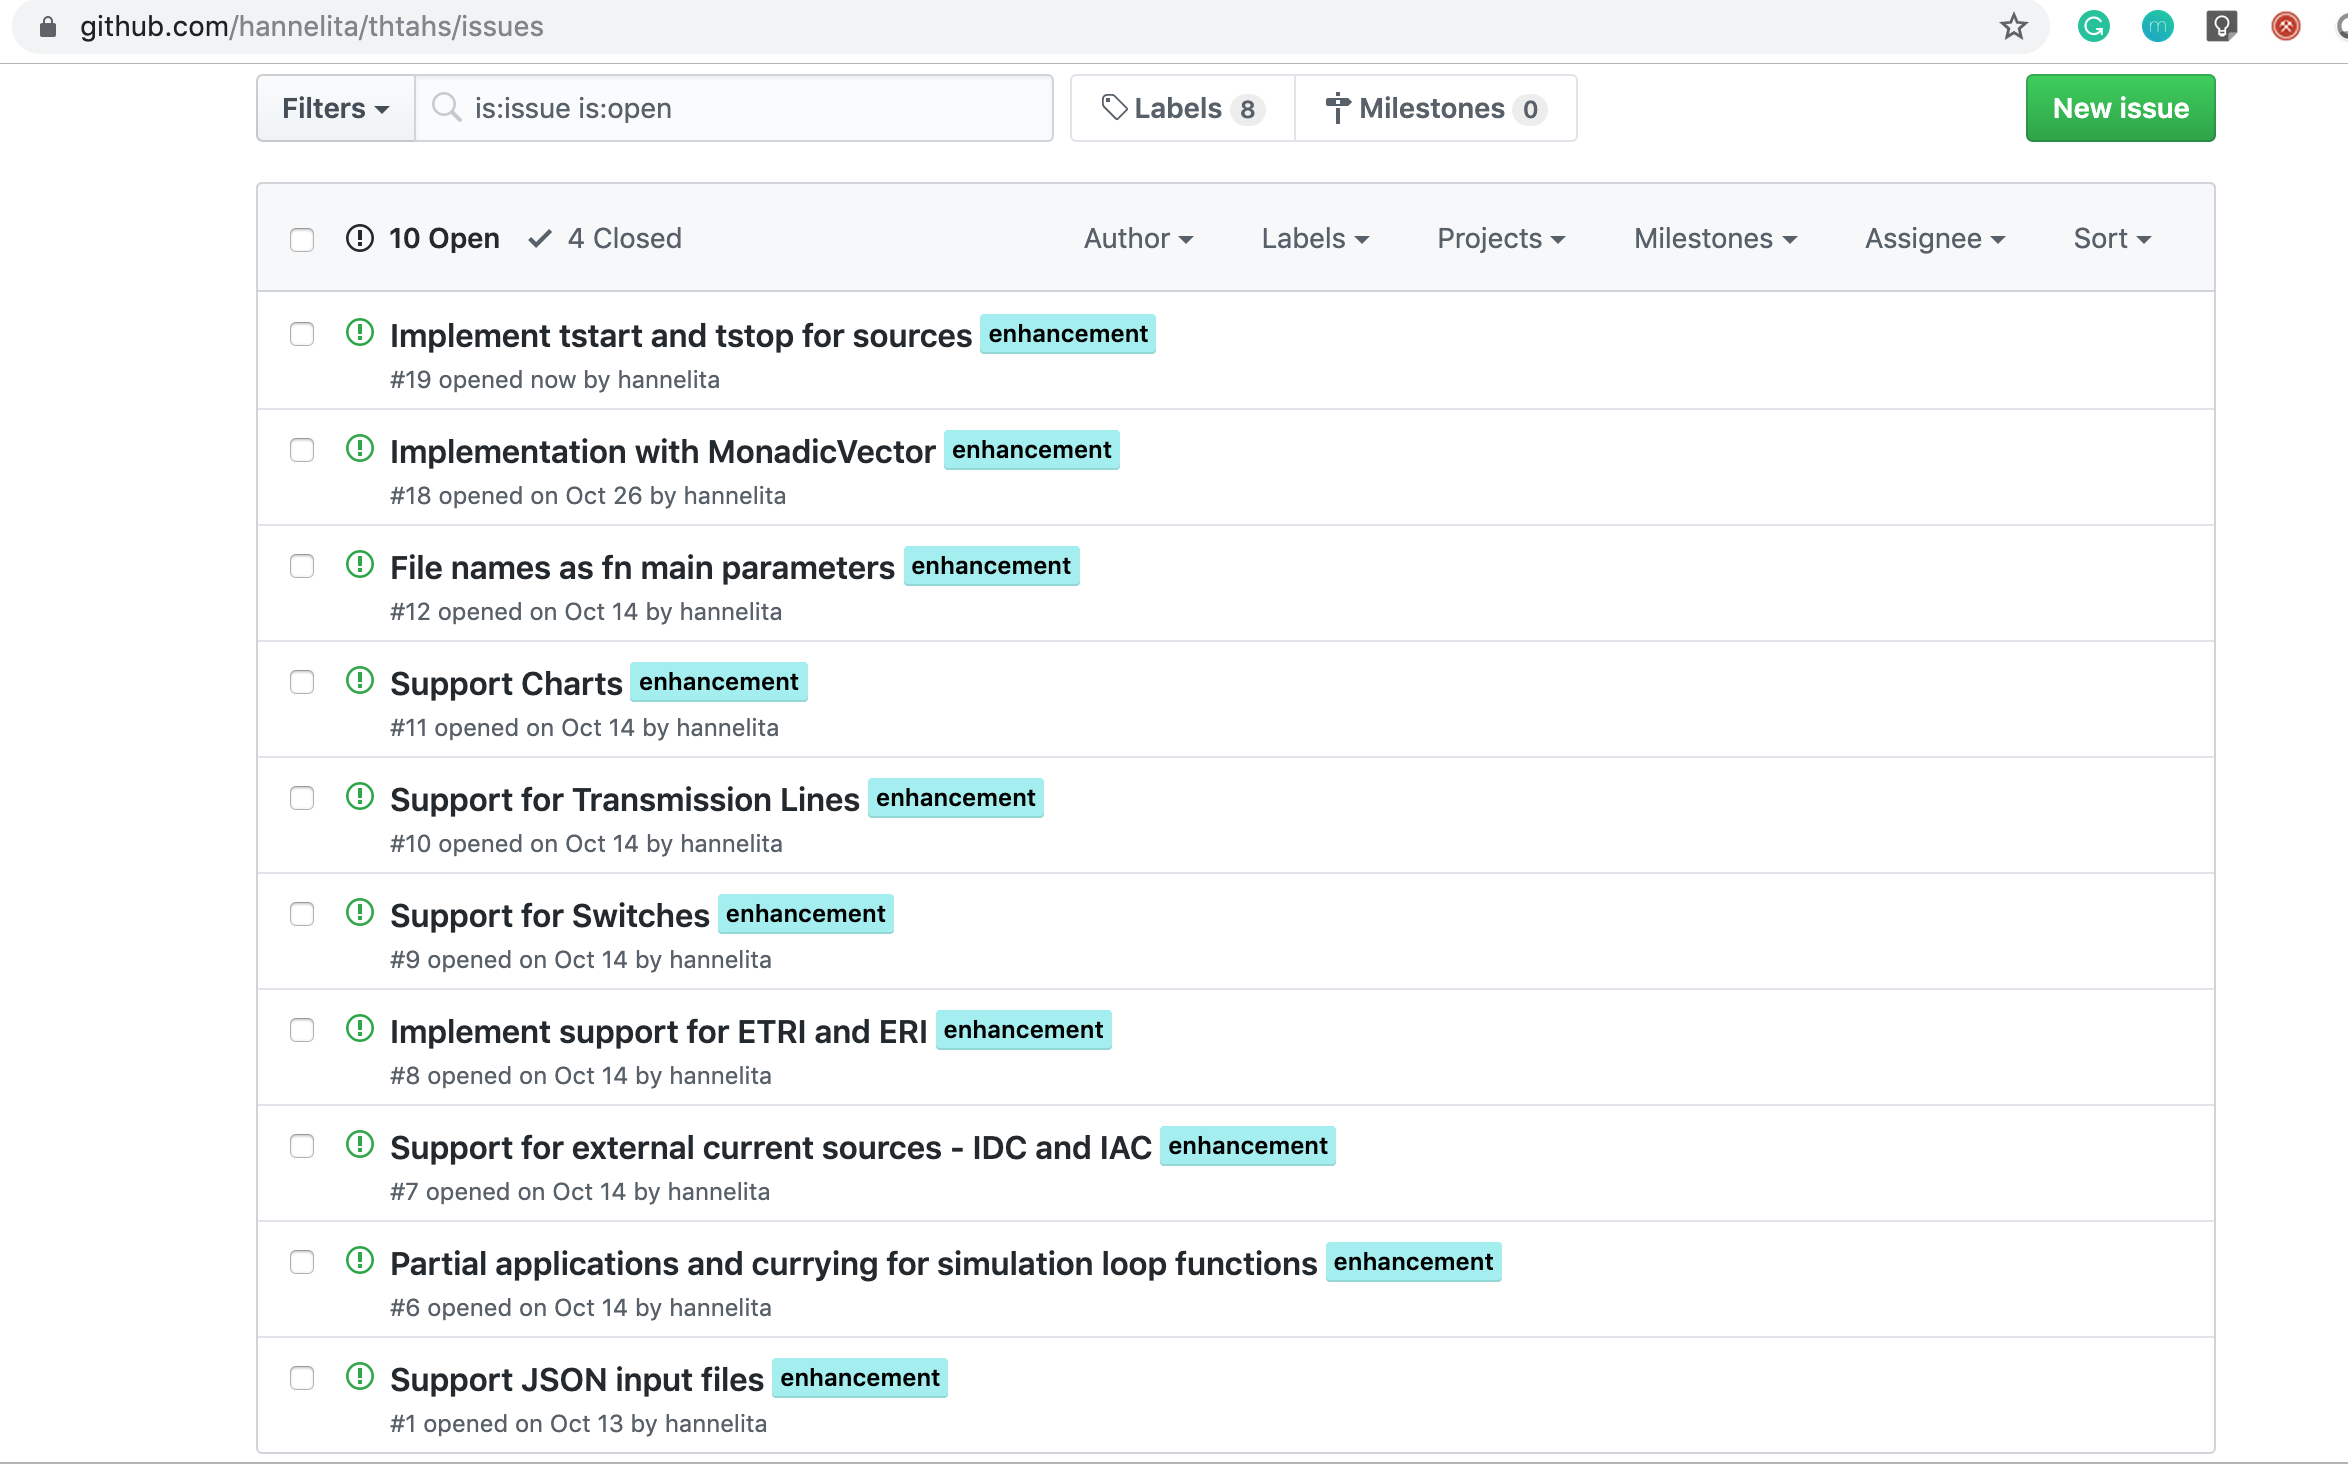
\includegraphics[width=0.7\textwidth]{img/featuresgithub.png}
   \caption{Issue tracker on Github for the Haskell ETR-P project.}
   \label{fig:featuresgithub}
\end{figure}

\section{Final thoughts}

This work was deeply related with abstraction and types. In fact, abstracting the code and abstracting the engineering model of the nodal equations were both joint into the implementation of this Haskell code. By finding ways to abstract the code, it is possible to find more concise ways to represent and explain the physical model. From the equation $[G][V] = [Ih]$ in chapter \ref{ch:etr} to the main Haskell function signature in chapter \ref{implhs} \lstinline!thtaSimulation :: Vector ComponentData -> SimulationData -> SimulationResults! a lot of abstration was built. Are these two representations equivalent? This work does not provide any proof of it. But it provides the reader with the formal and technical tools to give an intuition on how to investigate this matter. 




\cleardoublepage
\chapter*{ Academic works }
\addcontentsline{toc}{chapter}{Academic Works}
\label{academic}

\section*{Publications}

Tavante HC, Bonatto BD, Coutinho MP. Open Source Implementations of Electromagnetic Transient Algorithms. In 2018 13th IEEE International Conference on Industry Applications (INDUSCON) 2018 Nov 12 (pp. 825-828). IEEE.

\section*{Participation in Conferences}

\begin{itemize}
  \item Programming Languages Mentoring Workshop (PLMW) at ICFP 2018 \url{https://icfp18.sigplan.org/track/PLMW-ICFP-2018}
  \item Student Volunteer at Principles of Programming Languages (POPL) 2019 \url{https://popl19.sigplan.org}
  \item Student Volunteer at European Conference on Object-Oriented Programming (ECOOP) 2019 \url{https://2019.ecoop.org}
  \item Student Volunteer at International Conference of Functional Programming (ICFP) 2019 \url{19.sigplan.org}
\end{itemize}

\cleardoublepage
% \input{}
% \cleardoublepage
% \input{}
% \cleardoublepage
% ...


% Appendix______________________________________________________________________
% \appendix
% \chapter{Lambda Calculus And History of Functional Programming}
\label{sec:lc}

\section{Lambda Calculus basics}
\label{sec:apdxbasicsls}

The roots of functional programming are strictly connected with mathematical logic (see Appendix \ref{sec:logic} for more information). The formalisation of the predicate calculus allowed functions to generalize operations since this type of logic allowed non-logical values (like numbers or strings) in its predicates. Quantifiers ($ \exists $ and $ \forall $) granted the analysis of sequences, essential for the formalisation of lists and other functional data structures (see \cite{okasaki1999purely}). With the advances in number theory (especially the ones proposed by G. Peano), it was possible to see the relationship between induction and recursion. As \cite{michaelson2011introduction} describes in his work, Russel and Withehead, then Hilbert, then G\"{o}del pushed logics and mathematical foundations forward, giving the first steps to the \textbf{theory of computability}.

Three distinct formal approaches to the theory of computability were proposed in the 1930s: \textit{Turing machines}, by A. Turing (see \cite{boolos2002computability} for further details), \textit{recursive function theory}, by S. Kleene and the \textit{Lambda calculus} (or $ \lambda$-calculus), by A. Church. All these three approaches are equivalent to each other. They are all able to generalise von Neumann's machines (digital computers). Turing machines are based on assignments and time-ordered evaluation. The other techniques treat computations as structured function application. 

In the 1960s, the LISP language is created, inspired by the $\lambda$ calculus. Even though LISP is a straightforward language, it built up the idea of translating high-level functional languages (such as Haskell) in a notation equally simple, based on the lambda-calculus \cite{peyton1987implementation}. The $\lambda$ calculus is based on function abstractions (which generalise expressions) and on function application (which perform the evaluation of the expressions). The name "calculus" is not in vain - it has properties and rules to describe programming languages. The abstraction of $\lambda$ can "be treated as a universal machine code for programming languages" \cite{michaelson2011introduction}. \ref{apdx:lambdaexpr} brings an example of the notation in the $\lambda$ calculus.

\begin{lstlisting}[caption={Lambda abstraction}, captionpos=b, mathescape=true, label={apdx:lambdaexpr}]
  ( $\lambda$ x . + x 1)
\end{lstlisting}

In \ref{apdx:lambdaexpr}, the $\lambda$ indicates a function, with one variable (\lstinline!x!), just as the mathematical expression $f(x)$ represents a single-variable function. The dot \lstinline!.! represents the beginning of the body of the function, just as the $=$ in maths. Then an expression in prefix form (operator, operands) shows up; in this case, \lstinline!+ x 1!, meaning that this function adds one to the variable \lstinline!x!. \lstinline!x! is called \textbf{bound variable}; it works like a place-holder and will be replaced by an argument when this expression is evaluated. In \cref{apdx:freeboundvar}, $4$ is the argument. It is also possible to see another component, \lstinline!y!, which is called \textbf{free variable}.

\begin{lstlisting}[caption={Free variable: y; Bound Variable: x}, captionpos=b, mathescape=true, label={apdx:freeboundvar}]
  ( $\lambda$ x . + x y) 4
\end{lstlisting}

\textbf{Beta-reduction} (Or $\beta$-reduction) is the operation of applying an argument to an expression (\ref{apdx:betareduction}).

\begin{lstlisting}[caption={Beta reduction}, captionpos=b, mathescape=true, label={apdx:betareduction}]
  ( $\lambda$ x . + x 1) 4 $\rightarrow $ (+ 4 1)
\end{lstlisting}

The $\beta$-reduction can be used "backwards", composing a $\beta$-abstraction \ref{apdx:betaabstraction}. The set of $\beta$ reduction/abstraction is know as $\beta$-conversion.

\begin{lstlisting}[caption={Beta abstraction}, captionpos=b, mathescape=true, label={apdx:betaabstraction}]
  (+ 4 1) $\leftarrow $  ( $\lambda$ x . + x 1) 4 
\end{lstlisting}

Intuitively, there is also an $\alpha$-conversion. This operation refers to variable name substitution, keeping the operations equivalent \ref{apdx:alphaconversion}.

\begin{lstlisting}[caption={Alpha conversion}, captionpos=b, mathescape=true, label={apdx:alphaconversion}]
  ( $\lambda$ x . + x 1) $\longleftrightarrow_{ \alpha }$ ( $\lambda$ y . + y 1) 
\end{lstlisting}

Expressions can behave equivalently with slightly different bodies when applied to the same arguments. The Eta-conversion (or $\eta$-conversion) is the rule describing this scenario \ref{apdx:etaconversion}.

\begin{lstlisting}[caption={Eta conversion}, captionpos=b, mathescape=true, label={apdx:etaconversion}]
  ( $\lambda$ x . + x 1) $\longleftrightarrow_{ \eta }$ ( + 1) 
\end{lstlisting}

There are other rules, but this Appendix will be restricted to these three, which are the most essential for the $\lambda$-calculus. After applying these rules, if an expression does not contain any other sub-expressions to be reduced, this expression is in the \textbf{Normal Form}, or NF, for short. There are several strategies to reduce an expression. Only some paths lead to normal form. A guaranteed strategy to reach the NF of an expression of the \textbf{Normal Order Reduction}. It specifies that "the leftmost, outermost redex should be reduced first" \cite{peyton1987implementation}. An outermost evaluation may require extra steps, but it will terminate if there is any path that leads the program to terminate.

There are multiple ways to analyse a function in terms of its semantics, listed in \ref{apdx:semantics} \cite{pierce2002types}.

\begin{enumerate}\label{apdx:semantics}
  \item Interpreting the function as a sequence of operations in time, analysing it under operational aspects. This is a 'dynamic' view of the function, called \textbf{operational semantics}. This type of semantics specifies an abstract machine. A state relates to a term, and a behaviour relates to the transition function.
  \item Interpret the function 'statically' as a set of arguments and values to be determined. This is called \textbf{Denotational semantics}. The meaning of a term is a mathematical object. It assigns a value to every expression in the language.
  \item \textbf{Axiomatic semantics} states that the meaning of a term is what can be proved about it.
\end{enumerate} 

The $\lambda$-calculus can be taken into operational and denotational definitions. Denotational semantics is essential because it allows reasoning about the termination of evaluation (formally represented by $ \perp $).

When a function needs the value of its argument, it is said to be \textit{strict}. The opposite, the function that does not request the value of its arguments, is called \textit{lazy}.

Lambda-Calculus is a vast topic and its content is much more extensive than the ones listed in \ref{sec:apdxbasicsls}. See \cite{barendregt2013lambda} and \cite{hindley2008lambda} for further references. 

\section{Translating programs into Lambda Calculus}

In section \ref{sec:apdxbasicsls}, the basic tools and principles of Lambda Calculus were presented in a summarised format. It is possible to translate codes written using the functional paradigm into Lambda-calculus. This is the first step to analyse code under a mathematical aspect. \cite{peyton1987implementation} suggests two approaches for the translation:

\begin{enumerate}
\item Perform successive transformations from one functional program to another, with a simplification in each step. The final simplified version of each function could, in theory, be translated to pure Lambda-Calculus. This approach focuses on syntax
\item Start by translating the program into an 'enriched' version of the Lambda-Calculus (a version of $\lambda$-calculus that includes the original one and additional features). From this enriched version, perform simplifications until reaching the simple version of the $\lambda$-calculus. This approach focuses on semantics.
\end{enumerate}

This work will not describe these techniques in-depth, nor implement such translation.




% \cleardoublepage
% \chapter{Logic and Mathematics}
\label{sec:logic}

In order to analyse the functional code as a mathematical object, it is important to think about an appropriate Logic. In classical mathematics, \textbf{Propositional Logic} uses connectives (and, or, not, etc) to validate tautologies through proofs (or derivations). A complete guide to all propositional logic domain (such as signed formulas, construction of tableaux, logical consequence analysis, axioms, correctness, completeness and compactness) can be found at \cite{smullyan2014beginner}. This type of logic is limited to a proposition and connectives, which (for a well formed formula) will be either true or false.

\textbf{Predicate Logic}, or First Order Logic, adds two important components to the analysis - the existential quantifiers $ \forall $ and $ \exists $ and the introduction of variables to the predicates (example: $ \exists x Gx $). This type of logic has some similarities with the $\lambda $-Calculus (see \ref{sec:lc}), such as the occurrence of free and bound variables and substitution rules. 

Are there any other types of logic which would be more suitable for analysing programs? It is necessary to dig into mathematics to try to answer this question. It might be necessary to take some of the foundations of mathematics into consideration. Frege made a few, unsuccessful attempts to create an 'arithmeticization' of analysis (\cite{george2002philosophies}). For Frege, logic is the study of truth-preserving inferences and concepts are ontological counterparts of predicative expressions. Concepts are functions from objects to truth values. A concepts can be categorized as:

\begin{itemize}
  \item \textbf{First-level concepts} - Obtained by removing a name from a declarative sentence, originating a \textit{first level predicate}. 
  \item \textbf{Recognition statements} - since any expression can be part of infinitely many sentences, a recognition statement is a concept acting as a wild-card for this case. 
  \item \textbf{Equivalence relations} - Frege's logicism aims to build gap-free demonstrations by partitioning the universe in clusters by equinumerosity. This analysis is a recursive characterization of natural numbers (which are clusters themselves). These clusters are equivalence relations.
\end{itemize}

Frege's model main concern arises of the need of logical objects. How to define these logical objects? Frege creates another concept, the \textbf{extensions}. By proposing that every object has an extension in an axiom, Frege runs into a paradox where some sets would be member of themselves and some wouldn't, creating an inconsistency in his general proposal. This is widely known as \textbf{Russel's paradox}. 

Russel and Withehead investigated this matter and proposed an alternative, the \textit{Ramified Theory of Types}, which does not rely on sets, but on propositional functions. In this theory, all objects are classified into a hierarchy of types. Unfortunately, this approach bans unharmful sets (paradox-free). Most mathematicians prefer to use alternative theories of sets which are free of paradox and do not require the classification of all entities into types. The most popular model following this proposals is the ZFC (Zermelo-Frankel and the Axiom of Choice model). Note that ZFC is only concerned about sets, whereas Russel's main goal is to show how logic can be applied to general statements. ZFC is a formal axiomatic theory: there is a language to write statements. There is no guarantee that ZFC is paradox-free (no proof it is consistent).

These models presented previously somehow rely on the idea of a set. But a set might have issues according to realism. In philosophy, \textit{realism} states that some propositions might be nor true of false: there is no known answer. The \textit{Law of the Excluded Middle} (wither S is true or not-S is true) might not be valid. The "anti-realist" conception of mathematics is called \textbf{constructivism}. \textbf{Intuitionism} is one type of constructivism, which suggests that mathematical reality is not fully fixed. Infinitude is potential. Intuitionism contasts with classical mathematics and logic for not accepting infinites (see \cite{weyl2013levels}), nor requiring a true/false result.

Intuitionistic mathematics has its own rules, and some of the axioms of the classical logic become invalid under the intuitionistic perspective. When analysing programs, this is one type of logic that could be a potential candidate for adoption. In practical terms, the classical mathematician has a fixed mathematical reality and an actual infinite. The intuitionistic determines a potential infinite. Translating these differences to proofs, the intuitionistic model has the advantage of establishing finite proofs (which are fairly desirable when aiming to termination). Intuitionism imposes constraints to the universal quantifier $ \forall $. In intuitionism, the double negation elimination is not valid:

\begin{prooftree}\label{proofintuit}
  \AxiomC{$\neg \neg X $}
  \UnaryInfC{$ X $}
\end{prooftree}

In contrast, there is an intuitionistic version which is valid:

\begin{prooftree}\label{proofintuitvalid}
  \AxiomC{$X \lor \neg X $}
  \AxiomC{$\neg \neg X $}
  \BinaryInfC{$ X $}
\end{prooftree}

This chapter does not brings the topic of constructive mathematics in detail, but when combined with functional programming, $\lambda$-calculus and logic, it becomes the baseline for Type Theory, quickly described in \ref{sec:proofs}. Using the words of \cite{thompson1991type} to summarise the relevance of this appendix, "the short discussion of constructive mathematics introduced the idea that proofs should have computational content; [...] to achieve this goal, the underlying logic of the system needed to be changed to one in which we only assert the validity of a proposition when we have a proof of the proposition."



% \cleardoublepage
% \chapter{Types and Proofs}
\label{sec:proofs}

A type system is a tool for reasoning about programs. When built using the appropriate logic system, it can avoid paradoxes such as Russel's paradox (\ref{sec:logic}). Type systems help to eliminate run-time errors, by catching inconsistencies (paradoxes) in compile time. In order to analyse functions at this level, it is necessary to see programs as proofs. This Appendix will briefly explore the duality between propositions and types, proofs and elements. A proof of a proposition T is isomorphic to the type T. "a proof by induction is nothing other than a proof object defined using recursion" \cite{thompson1991type}. A program then becomes a set of terms built by the elements in a certain grammar. From there, it is possible to derive the necessary inference rules. It is with the aid of $\lambda$-calculus that the syntax of the language is analysed and transformed into an abstract syntax tree (AST).

This process of formalizing types is detailed described in \cite{pierce2002types}. As an example, the (simply-typed) $\lambda$-Calculus over the type Bool if described as \ref{boolsimplytyped}.

\begin{subequations}\label{boolsimplytyped}
\begin{equation}
    T ::= 
\end{equation}
\begin{equation}
    Bool
\end{equation}
\begin{equation}
    T \rightarrow T
\end{equation}
\end{subequations}

This process is extended to all of the base types in the language (such as Integer, Float, Char, etc), as well as collections (Lists, Tuples, etc). Impure functions and exceptions also have corresponding types. The relation between types is also analysed, such as subtyping and polymorphism.

This appendix could bring an extensive buzzword list (recursive types, equi-recursive types, type reconstruction, Universal types, existential types, higher order polymorphism, dependent types). Explaining these concepts in detail is out of the scope of this work, but asking which system would best describe (in terms of paradox-free and expressiveness) the implemented software is a pertinent question. A wider comparison between implementations using the formalism of type theory is a future work. To conclude this brief appendix, it is possible to quote \cite{thompson1991type}: "There is still much to be done in making type theory a usable and attractive system which supports programming in the large, but I am certain that languages based on type theory will be as popular in a few years as contemporary functional languages".





% \cleardoublepage
% \chapter{Haskell ETR-P source code}
\label{apdx:code}

Source code for the \lstinline!main.hs! file.

\begin{lstlisting}[language=Haskell, numbers=left, caption={Main.hs file code}, captionpos=b, label={lst:maincompletecode}]
{-# LANGUAGE OverloadedStrings #-}
{-# LANGUAGE RecordWildCards #-}

module Main where
import qualified Data.Foldable as Foldable

-- vector
import Data.Vector (Vector)
import qualified Data.Vector as Vector

-- Matrix
import Data.Matrix (Matrix)
import qualified Data.Matrix as Matrix

-- HMatrix
import qualified Numeric.LinearAlgebra.Data as HMatrix
import qualified Numeric.LinearAlgebra.HMatrix as HMatrix

-- bytestring
import Data.ByteString.Lazy (ByteString)
import qualified Data.ByteString.Lazy as ByteString

-- cassava
import Data.Csv
  ( DefaultOrdered(headerOrder)
  , FromField(parseField)
  , FromNamedRecord(parseNamedRecord)
  , Header
  , ToField(toField)
  , ToNamedRecord(toNamedRecord)
  , (.:)
  , (.=)
  )
import qualified Data.Csv as Cassava

-- text
import Data.Text (Text)
import qualified Data.Text.Encoding as Text

-- Exception
import Control.Exception

-- base
import qualified Control.Monad as Monad
import qualified System.Exit as Exit
import qualified Debug.Trace as Trace



data ComponentData = 
  ComponentData { 
    componentType :: ComponentType,
    nodeK :: Int,
    nodeM :: Int,
    magnitude :: Double,
    param1 :: Double,
    param2 :: Double,
    plot :: Int
     }
  deriving (Eq, Show)


data SimulationData = 
  SimulationData { 
    nodes :: Int,
    voltageSources :: Int,
    stepSize :: Double,
    tmax :: Double
     }
  deriving (Eq, Show)

data ComponentType = Resistor | Capacitor | Inductor | EAC | EDC | Other Text deriving (Eq, Show)
type SimulationResults = (Vector Double, Matrix Double)

instance FromNamedRecord SimulationData where
  parseNamedRecord m =
    SimulationData
      <$> m .: "Number of Nodes"
      <*> m .: "Number of Voltages Sources"
      <*> m .: "Step Size"
      <*> m .: "Maximum time for simulation"


instance FromNamedRecord ComponentData where
  parseNamedRecord m =
    ComponentData
      <$> m .: "Element Type"
      <*> m .: "Node K"
      <*> m .: "Node M"
      <*> m .: "Value"
      <*> m .: "Source param 1"
      <*> m .: "Source param 2"
      <*> m .: "Plot"

instance FromField ComponentType where
  parseField "R" =
    pure Resistor

  parseField "L" =
    pure Inductor

  parseField "C" =
    pure Capacitor

  parseField "EDC" =
    pure EDC

  parseField "EAC" =
    pure EAC

  parseField otherType =
    Other <$> parseField otherType


decodeItems :: ByteString -> Either String (Vector ComponentData)
decodeItems =
  fmap snd . Cassava.decodeByName

decodeItemsFromFile :: FilePath -> IO (Either String (Vector ComponentData))
decodeItemsFromFile filePath =
  catchShowIO (ByteString.readFile filePath)
    >>= return . either Left decodeItems

decodeSimulation :: ByteString -> Either String (Vector SimulationData)
decodeSimulation =
  fmap snd . Cassava.decodeByName

decodeSimulationFromFile :: FilePath -> IO (Either String (Vector SimulationData))
decodeSimulationFromFile filePath =
  catchShowIO (ByteString.readFile filePath)
    >>= return . either Left decodeSimulation

getSingleSimulationLine :: Vector SimulationData -> SimulationData
getSingleSimulationLine = 
    Vector.head 


nhComponents :: [ComponentData] -> [ComponentData]
nhComponents =
  filter (\r -> (componentType r == Capacitor) || (componentType r == Inductor))

filterEnergyStorageComponent :: Vector ComponentData -> Vector ComponentData
filterEnergyStorageComponent =
  Vector.filter (\r -> (componentType r == Capacitor) || (componentType r == Inductor))

nh :: Vector ComponentData -> Int
nh components =
  length $ filterEnergyStorageComponent components
    
filterSources :: Vector ComponentData -> Vector ComponentData
filterSources =
  Vector.filter (\r -> (componentType r == EDC) || (componentType r == EAC))

condutance :: ComponentData -> Double -> Double
condutance component dt =
  case componentType component of
    Resistor -> 1.0 / (magnitude component)
    Capacitor -> (magnitude component) * 0.000001 * 2 / dt
    Inductor -> dt / (2 * 0.001 * (magnitude component))
    _ -> 0.0

gkm :: Vector ComponentData -> Double -> Vector Double
gkm components dt =
  Vector.map (\c -> condutance c dt) components

buildCompactGMatrix :: Double -> [ComponentData] -> Matrix Double -> Matrix Double
buildCompactGMatrix dt [] buffer = buffer
buildCompactGMatrix dt (component:cs) buffer =
  case (nodeK component, nodeM component) of 
    (0, m) -> buildCompactGMatrix dt cs (Matrix.setElem (Matrix.getElem m m buffer + condutance component dt) (m, m) buffer)
    (k, 0) -> buildCompactGMatrix dt cs (Matrix.setElem (Matrix.getElem k k buffer + condutance component dt) (k, k) buffer)
    (k, m) -> buildCompactGMatrix dt cs (Matrix.setElem (Matrix.getElem k k buffer + condutance component dt) (k, k) (Matrix.setElem (Matrix.getElem m m buffer + condutance component dt) (m, m) (Matrix.setElem (Matrix.getElem k m buffer - condutance component dt) (k, m) (Matrix.setElem (Matrix.getElem m k buffer - condutance component dt) (m, k) buffer))))
    (_, _) -> buildCompactGMatrix dt cs buffer


buildGMatrixFromVector :: SimulationData -> Vector ComponentData -> Matrix Double
buildGMatrixFromVector simulation components =
  buildCompactGMatrix (stepSize simulation) (Vector.toList components) (Matrix.zero (nodes simulation) (nodes simulation))


buildIhVector :: [ComponentData] -> Double -> Int -> [Double] -> [Double] -> Matrix Double -> Vector Double
buildIhVector [] _ _ _ ihnew _ = Vector.fromList ihnew
buildIhVector (component:cs) dt n (hold:ihold) ihnew vMatrix =
  case (componentType component, nodeK component, nodeM component) of 
    (Inductor, 0, m) -> buildIhVector cs dt n ihold (ihnew ++ [(2*(condutance component dt)*(Matrix.getElem m n vMatrix) + hold)]) vMatrix
    (Inductor, k, 0) -> buildIhVector cs dt n ihold (ihnew ++ [(-2*(condutance component dt)*(Matrix.getElem k n vMatrix) + hold)]) vMatrix
    (Inductor, k, m) -> buildIhVector cs dt n ihold (ihnew ++ [(-2*(condutance component dt)*((Matrix.getElem k n vMatrix) - (Matrix.getElem m n vMatrix)) + hold)]) vMatrix
    (Capacitor, 0, m) -> buildIhVector cs dt n ihold (ihnew ++ [(-2*(condutance component dt)*(Matrix.getElem m n vMatrix) - hold)]) vMatrix
    (Capacitor, k, 0) -> buildIhVector cs dt n ihold (ihnew ++ [(2*(condutance component dt)*(Matrix.getElem k n vMatrix) - hold)]) vMatrix
    (Capacitor, k, m) -> buildIhVector cs dt n ihold (ihnew ++ [(2*(condutance component dt)*((Matrix.getElem k n vMatrix) - (Matrix.getElem m n vMatrix)) - hold)]) vMatrix
    (_, _, _) -> buildIhVector cs dt n ihold ihnew vMatrix



buildVBVector :: [ComponentData] -> Double -> [Double] -> Vector Double
buildVBVector [] _ buffer = Vector.fromList buffer
buildVBVector (c:components) time buffer =
  case (componentType c) of EDC -> buildVBVector components time ((magnitude c) : buffer)
                            EAC -> buildVBVector components time (((magnitude c * cos (2 * pi * param2 c * time + (param1 c * (pi/180))))) : buffer)
                            _   -> buildVBVector components time buffer


buildIVector :: [ComponentData] -> [Double] -> Vector Double -> Vector Double
buildIVector [] _ iVector = iVector
buildIVector (component:cs) (ihEl:ih) iVector =
  case (componentType component, nodeK component, nodeM component) of 
    (Inductor, k, 0) -> buildIVector cs ih (iVector Vector.// [((k - 1), ((iVector Vector.! (k-1)) + ihEl))])
    (Inductor, 0, m) -> buildIVector cs ih (iVector Vector.// [((m - 1), ((iVector Vector.! (m-1)) - ihEl))])
    (Inductor, k, m) -> buildIVector cs ih (iVector Vector.// [((m - 1), ((iVector Vector.! (m-1)) - ihEl)), ((k-1), ((iVector Vector.! (k-1)) + ihEl))])
    (Capacitor, k, 0) -> buildIVector cs ih (iVector Vector.// [((k - 1), ((iVector Vector.! (k-1)) + ihEl))])
    (Capacitor, 0, m) -> buildIVector cs ih (iVector Vector.// [((m - 1), ((iVector Vector.! (m-1)) - ihEl))])
    (Capacitor, k, m) -> buildIVector cs ih (iVector Vector.// [((m - 1), ((iVector Vector.! (m-1)) - ihEl)), ((k-1), ((iVector Vector.! (k-1)) + ihEl))])
    (_, _, _) -> buildIVector cs ih iVector


thtaControl :: Int -> Double -> Vector Double -> Vector Double -> SimulationData -> (Int, Vector Double, Double)
thtaControl thtactl time ihnew ih simulation
  | thtactl <= 0 = (thtactl, ihnew, (stepSize simulation + time))
  | thtactl < 3 = (thtactl + 1, (Vector.map (\i -> i/2) $ Vector.zipWith (+) ih ihnew), (time + (stepSize simulation/2)))
  | otherwise = (0, ihnew, (stepSize simulation + time))

fromHMatrixTransformer :: HMatrix.Matrix Double -> Matrix Double
fromHMatrixTransformer matrix =
  Matrix.fromLists $ HMatrix.toLists matrix

toHMatrixTransformer :: Matrix Double -> HMatrix.Matrix Double
toHMatrixTransformer matrix =
  HMatrix.fromLists $ Matrix.toLists matrix

fromHMatrixVectorTransformer :: HMatrix.Vector Double -> Vector Double
fromHMatrixVectorTransformer vec =
  Vector.fromList $ HMatrix.toList vec

toHMatrixVectorTransformer :: Vector Double -> HMatrix.Vector Double
toHMatrixVectorTransformer vec =
  HMatrix.fromList $ Vector.toList vec

solver :: HMatrix.Vector Double -> HMatrix.Matrix Double -> HMatrix.Matrix Double -> HMatrix.Matrix Double -> HMatrix.Matrix Double -> HMatrix.Vector Double -> SimulationData -> (Vector Double, Vector Double)
solver iVector gaa gab gba gbb vb simulation =
  let ia = HMatrix.subVector 0 ((nodes simulation) - (voltageSources simulation)) iVector
      rhsa = ia - (gab HMatrix.#> vb)
      va = gaa HMatrix.<\> rhsa
      ib = (gba HMatrix.#> va) + (gbb HMatrix.#> vb)
      iVec = HMatrix.vjoin [ia, ib]      
      vVec = HMatrix.vjoin [va, vb]
  in
    ((fromHMatrixVectorTransformer iVec), (fromHMatrixVectorTransformer vVec))
      

thtaSimulationStep :: [ComponentData] -> Matrix Double -> SimulationData -> Int -> Int -> Double  -> Vector Double -> Matrix Double -> Vector Double -> Vector Double -> SimulationResults
thtaSimulationStep _ _ _ _ 1 _ _ vMatrix _ iVector = (iVector, vMatrix)
thtaSimulationStep components condutances simulation thtactl n time ih vMatrix vbVector iVector =
  let (gaa, gab, gba, gbb) = Matrix.splitBlocks (nodes simulation - voltageSources simulation) (nodes simulation - voltageSources simulation) condutances
      ihBuffer = buildIhVector (nhComponents components) (stepSize simulation) n (Vector.toList ih) [] vMatrix
      (thta, ihThta, timeThta) = thtaControl thtactl time ihBuffer ih simulation
      vbVec = buildVBVector components timeThta []
      iVec = buildIVector (nhComponents components) (Vector.toList ihThta) (Vector.replicate (nodes simulation) 0)
      (iVecCalc, vVec) = solver (toHMatrixVectorTransformer iVec) (toHMatrixTransformer gaa) (toHMatrixTransformer gab) (toHMatrixTransformer gba) (toHMatrixTransformer gbb) (toHMatrixVectorTransformer vbVec) simulation
      vMatr = Matrix.mapCol (\r _ -> vVec Vector.! (r - 1)) (n-1) vMatrix
  in
      thtaSimulationStep components condutances simulation thta (n-1) timeThta ihThta vMatr vbVec iVecCalc


thtaSimulation :: Vector ComponentData -> SimulationData -> SimulationResults
thtaSimulation components simulation = 
  thtaSimulationStep (Vector.toList components) (buildGMatrixFromVector simulation components) simulation 1 (npoints simulation) 0.0 (Vector.replicate (nh components) 0) (Matrix.zero (nodes simulation) (npoints simulation)) (Vector.replicate (voltageSources simulation) 0) (Vector.replicate (nodes simulation) 0)


npoints :: SimulationData -> Int
npoints sim = 
  round ((tmax sim)/(stepSize sim)) + 1

catchShowIO :: IO a -> IO (Either String a)
catchShowIO action =
  fmap Right action
    `catch` handleIOException
  where
    handleIOException :: IOException -> IO (Either String a)
    handleIOException =
      return . Left . show

main :: IO ()
main = do

  eitherSimulation <-
      fmap getSingleSimulationLine
        <$> decodeSimulationFromFile "data/simulation.csv"

  case eitherSimulation of
    Left reason ->
      Exit.die reason

    Right simulation -> do
      components_list <- decodeItemsFromFile "data/components.csv"
      case components_list of
        Left reason -> Exit.die reason
        Right components -> do
          let gmt = buildGMatrixFromVector simulation components
          putStr "GMatrix: \n"
          print (gmt)
          let results = thtaSimulation components simulation
          putStr "Simulation: \n"
          print (results)

\end{lstlisting}





% Bibliography__________________________________________________________________
% Literature (Additional references can be added to the .bib-file manually, or by using, for example, the free application JabRef). Compile in the following order: latex -bibtex -latex -latex

\bibliographystyle{ieeetr}
\bibliography{bibliography}

\end{document}
